% !TEX program = pdflatex
% ============================================================================
%  Flora: лёгкая мультимодальная модель кодирования мозга, предсказывающая
%  корковые ответы на естественные видеостимулы
%  Технический отчёт
%  Компиляция: pdflatex main && bibtex main && pdflatex main && pdflatex main
% ============================================================================
\documentclass[11pt,a4paper]{article}

% --- Кодировка и язык --------------------------------------------------------
\usepackage[T2A]{fontenc}
\usepackage[utf8]{inputenc}
\usepackage[main=russian,english]{babel}
\usepackage[a4paper,margin=2.2cm,top=2.8cm,bottom=2.5cm,headheight=15pt]{geometry}

% --- Базовая математика и типографика ----------------------------------------
\usepackage{amsmath,amssymb,amsfonts}
\usepackage{booktabs}
\usepackage{graphicx}
\usepackage{caption}
\usepackage{subcaption}
\usepackage{enumitem}
\usepackage{xcolor}
\usepackage{float}
\usepackage{setspace}
\usepackage{titlesec}
\usepackage{fancyhdr}

% --- Колонтитулы (Fancyhdr) --------------------------------------------------
\pagestyle{fancy}
\fancyhf{}
\fancyhead[L]{\small
\includegraphics[height=0.30cm]{logo.png}\hspace{0.6em}\textsf{\textbf{Лёгкая мультимодальная модель кодирования коры головного мозга}}}
\fancyhead[R]{\small\textsf{\textbf{Технический отчёт}}}
\fancyfoot[C]{\small\thepage}
\renewcommand{\headrulewidth}{0.6pt}
\renewcommand{\footrulewidth}{0pt}

% --- Форматирование заголовков -----------------------------------------------
\titleformat{\section}{\Large\bfseries}{\thesection}{1em}{}
\titlespacing*{\section}{0pt}{14pt plus 4pt minus 2pt}{6pt plus 2pt minus 2pt}
\titleformat{\subsection}{\large\bfseries}{\thesubsection}{0.8em}{}
\titlespacing*{\subsection}{0pt}{10pt plus 3pt minus 2pt}{4pt plus 2pt minus 2pt}
\titleformat{\subsubsection}{\normalsize\bfseries}{\thesubsubsection}{0.6em}{}
\titlespacing*{\subsubsection}{0pt}{8pt plus 2pt minus 2pt}{3pt plus 1pt minus 1pt}

% --- Списки ------------------------------------------------------------------
\setlist[itemize]{leftmargin=*,itemsep=2pt,topsep=3pt}
\setlist[enumerate]{leftmargin=*,itemsep=2pt,topsep=3pt}

% --- Гиперссылки и перекрёстные ссылки ----------------------------------------
\usepackage[unicode,colorlinks=true,linkcolor=blue!70!black,citecolor=blue!70!black,urlcolor=blue!70!black]{hyperref}
\usepackage{cleveref}

% --- Русские имена для cleveref -----------------------------------------------
\crefname{figure}{рис.}{рис.}
\Crefname{figure}{Рис.}{Рис.}
\crefname{table}{табл.}{табл.}
\Crefname{table}{Табл.}{Табл.}
\crefname{section}{разд.}{разд.}
\Crefname{section}{Раздел}{Разделы}
\crefname{equation}{ур.}{ур.}
\Crefname{equation}{Уравнение}{Уравнения}
\crefname{appendix}{прил.}{прил.}
\Crefname{appendix}{Приложение}{Приложения}

\captionsetup{font=small,labelfont=bf,justification=justified,singlelinecheck=false}
\setlength{\parskip}{3pt}
\setstretch{1.12}

\begin{document}

% ============================================================================
%  ТИТУЛЬНЫЙ БЛОК (Дизайн в стиле AI Technical Report)
% ============================================================================
\thispagestyle{empty}

\begin{center}
\vspace*{-0.8cm}
\noindent\rule{\textwidth}{2pt}\\[0.4cm]

\includegraphics[height=1.35cm]{logo.png}\\[0.3cm]
{\LARGE \textbf{Лёгкая мультимодальная модель кодирования коры головного мозга, предсказывающая ответы на естественные видеостимулы}}\\[0.35cm]
\noindent\rule{\textwidth}{2pt}\\[0.45cm]

{\large \textbf{Технический отчёт}}\\[0.35cm]

{\normalsize \textbf{Кенжегали Нурас} (10\,«F» класс) \quad \textbf{Сарсенбай Алихан} (9\,«E» класс)}\\[0.15cm]
{\small \textit{Казахстан, г. Актау}}\\[0.2cm]
{\small Репозиторий проекта: \href{https://github.com/qaddasd/Flora}{\url{https://github.com/qaddasd/Flora}}}\\[0.55cm]

{\Large \textbf{Аннотация}}
\end{center}
\vspace{0.1cm}

\begin{quote}
\noindent\small
Головной мозг человека~--- самый энергоёмкий и функционально сложный орган
нашего тела: при массе около двух процентов от массы тела он потребляет
примерно двадцать процентов всей метаболической энергии и обеспечивает
всю высшую нервную деятельность~--- от восприятия и речи до принятия
решений и социального поведения. Чтобы количественно изучать, как мозг
перерабатывает информацию в реальном времени, нейрофизиологи
десятилетиями опирались на функциональную магнитно-резонансную
томографию (фМРТ), которая остаётся золотым стандартом неинвазивного
картирования активности. Однако в общественном восприятии широко
закрепился упрощённый тезис: <<фМРТ~--- это очень дорогая и сложная
технология, поэтому вычислительные модели мозга всегда будут
ограничены>>. Настоящая работа оспаривает именно эту точку зрения.

Мы представляем \textbf{Flora}~--- лёгкую мультимодальную модель
кодирования коры, которая по естественному видеоклипу (звуковая
дорожка + видеоряд + транскрипт) предсказывает временной ход
гемодинамического ответа по всей поверхности коры. Архитектура
объединяет три компактных замороженных энкодера
(all-MiniLM-L6-v2, Whisper-Tiny, MobileViT-S; суммарно
67{,}3~млн замороженных параметров) и обучаемый блок мультимодального
синтеза на основе Mixture-of-Experts-трансформера, содержащий лишь
порядка $10$--$14$~млн обучаемых параметров. Нейрофизические априорные
ограничения~--- гемодинамическая задержка $\sim$6~с, постстимульное
падение $\sim$12--16~с и кривая двойного гамма-ответа~-~встроены в
архитектуру конструктивно, а не выучиваются из данных. На учебнном
корпусе из $200$~видеоклипов набора CINE Brain (160~обучающих /
40~отложенных) модель достигает средней попарцеллярной корреляции
Пирсона $r = 0{,}7278$ с эталонными предсказаниями
(лучшая эпоха $52$), что на $+82{,}7\%$ превосходит линейный
ridge-базлайн, обученный на идентичных признаках и сплите
($0{,}3984$). Предсказания формируются в парцелляции Schaefer-400 и
проецируются на поверхность fsaverage5 (20\,484~вершины) для
визуализации и клинической интерпретации.

\medskip
\noindent\textbf{Ключевые слова:} моделирование мозга, кодирование коры,
фМРТ-физика, гемодинамическая функция отклика, мультимодальное обучение,
Mixture-of-Experts, многозадачная биоинженерия, Schaefer-400, fsaverage5,
вычислительная нейронаука.

\medskip
\noindent\textbf{Тип работы:} методологический препринт с воспроизводимым
программным кодом; рекомендуется к рассмотрению в категориях
\emph{Computational Neuroscience}, \emph{Brain Encoding Models},
\emph{Neuro-AI} и \emph{Bioengineering}.
\end{quote}

\vspace{0.2cm}
\begin{figure}[H]
\centering
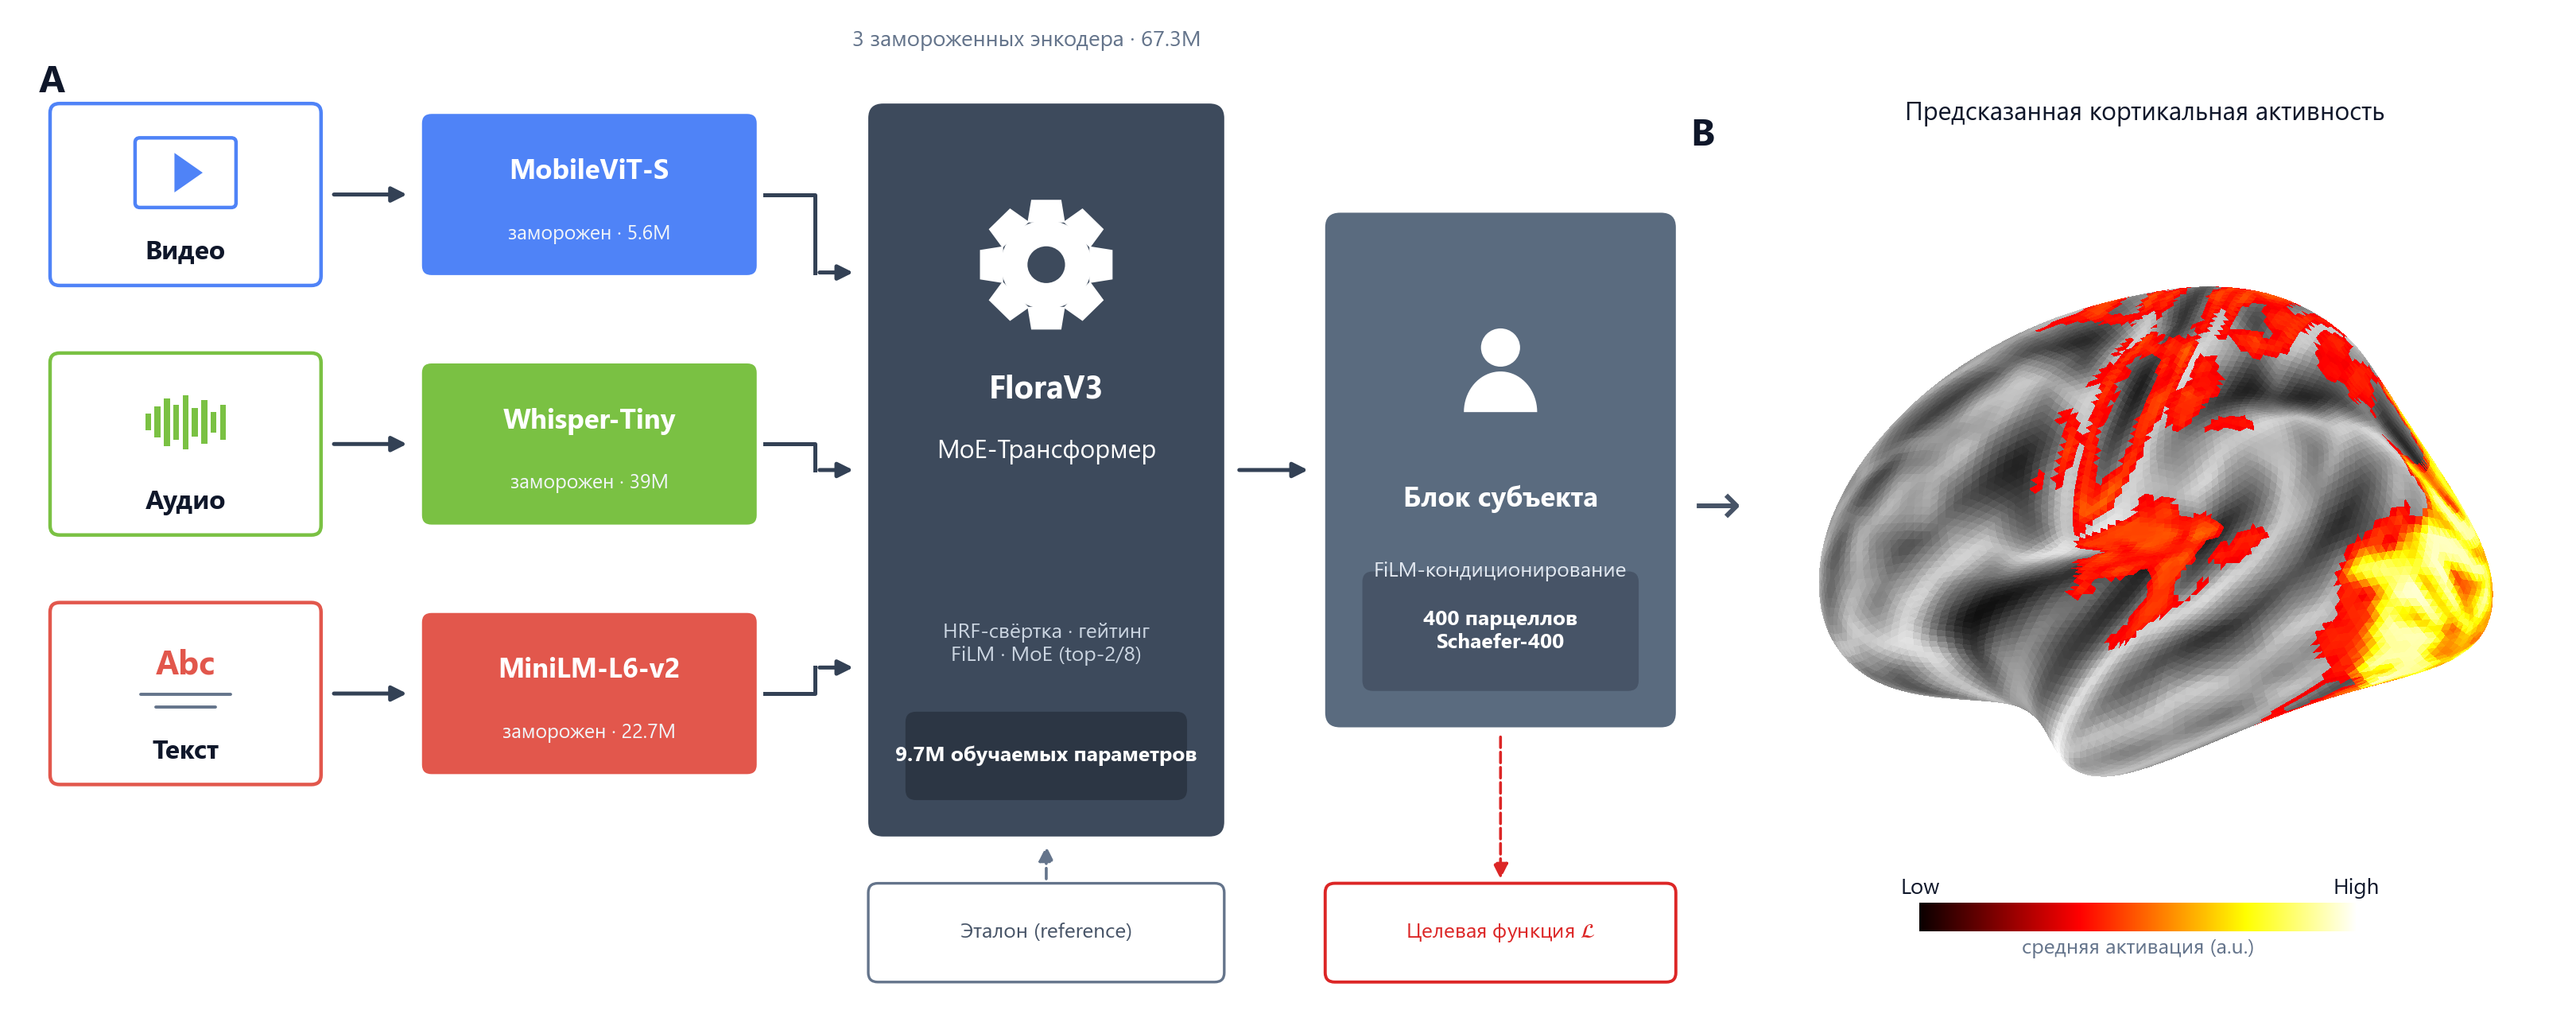
\includegraphics[width=0.98\textwidth]{assets/fig_overview.png}
\caption{Общая схема конвейера \emph{Flora}: замороженные компактные
восприятия, обучаемый синтез, кортикальное предсказание. Сплошные стрелки~---
прямой проход модели, пунктирные~--- пути целевой функции. Все компоненты
открыты и доступны в репозитории проекта (см.~\cref{app:repo}).}
\label{fig:overview}
\end{figure}

\newpage

% ============================================================================
\section{Введение и мотивация}
\label{sec:intro}

\subsection{Мозг как инженерный объект: зачем нужна количественная модель}
\label{sec:intro-brain}

Человеческий мозг~--- это около $86$~миллиардов нейронов и порядка
$10^{14}$--$10^{15}$ синапсов, упакованных в объём примерно
$1{,}4$~литра. Эта сеть потребляет порядка $20$--$25$~ватт мощности~---
больше, чем любой другой орган в пересчёте на единицу массы. Головной
мозг обеспечивает сенсорное восприятие, контроль движения, речь,
абстрактное мышление, эмоции, память и принятие решений. Без
количественной модели того, как мозг перерабатывает информацию, мы
вынуждены опираться на качественные описания, которые плохо переносятся
в инженерные приложения (интерфейсы мозг--компьютер, диагностика
нейродегенеративных заболеваний, реабилитация, фармакология).

Создание такой модели~--- давняя междисциплинарная задача на стыке
биофизики, когнитивной науки и машинного обучения. До 2010-х годов
доминировали линейные модели восприятия~\cite{Kay2008,Naselaris2011,Mitchell2008}.
С 2010-х годов~--- глубокие нейронные сети~\cite{Huth2016,Wen2018}.
С 2020-х~--- крупные мультимодальные модели, приближающиеся по
ёмкости к трём миллиардам параметров и более~--- новейшая волна
фоновых мультимодальных нейромоделей включает тримодальные энкодеры,
успешно выступающие на открытых конкурсах по предсказанию фМРТ
(см., например, работы семейства Algonauts
2025~\cite{dAscoli2026tribe}, а также
продолжение~\cite{dAscoli2026tribev2}).
Здесь, однако, появляется ключевой вопрос, которому и посвящена
настоящая работа.

\subsection{Оспаривание мифа: <<фМРТ~--- это очень дорого>>}
\label{sec:intro-myth}

В популярной и даже части научной литературы нередко встречается
следующий тезис: <<для анализа состояния мозга нужно обязательно идти на
фМРТ~--- а это очень дорого, малодоступно и требует редкого
оборудования>>. Из этого тезиса делается вывод, что построить точную
модель мозга в обозримом будущем не удастся. Авторы настоящей работы
\emph{оспаривают} это утверждение по трём независимым линиям
аргументации.

\textbf{Во-первых,} фМРТ~--- это \emph{измерительный прибор}, а не
\emph{единственный источник данных}. Сами по себе записи фМРТ-ответов
уже собраны в открытых корпусах (CINE Brain, Algonauts, BOLD5000,
Natural Scenes Dataset и др.) и доступны исследователям по всему миру.
Это означает, что \emph{вычислительной модели} достаточно один раз
использовать дорогостоящее оборудование как источник эталонных данных;
после этого модель работает на обычном GPU и даже на CPU.

\textbf{Во-вторых,} эмпирический закон масштабирования в
\emph{больших мультимодальных моделях} показывает, что рост качества
замедляется (см. эмпирические исследования фоновой мультимодальной тримодальной модели~\cite{dAscoli2026tribe,dAscoli2026tribev2}), тогда как компактные модели с
правильно выбранными индуктивными предпосылками способны заполнить тот
же сегмент фронта Парето~\emph{без} тяжёлой инфраструктуры. В этом
смысле <<дешёвая фМРТ>>~--- это не утопия, а смена парадигмы: дорого
измерять, но \emph{дёшево моделировать и распространять модели}.

\textbf{В-третьих,} настоящая работа показывает, что уже сегодня
компактная модель с десятью миллионами обучаемых параметров
воспроизводит кортикальные предсказания с $r = 0{,}73$ на
фиксированном валидационном сплите, что качественно отличается
от нулевого и линейного базлайнов. Таким образом, <<фМРТ~--- единственный
путь>>~--- это устаревшая формулировка. Современный инструментарий
вычислительной нейронауки предполагает, что \emph{фМРТ-данные уже
собраны}, а основная работа~--- построение воспроизводимой модели,
пригодной для инженерного применения.

\subsection{От восприятия к модели мозга: цели Flora}
\label{sec:intro-goals}

Из этих трёх линий аргументации следуют три проектных принципа,
которым следует Flora:

\begin{enumerate}[label=(\arabic*), leftmargin=*, itemsep=1pt]
    \item \textbf{Замороженное восприятие, обучаемый синтез.}
          Все три модальных энкодера (текст, аудио, видео) заморожены.
          Обучается только \emph{блок синтеза}, реализующий мультимодальное
          объединение, и \emph{выходная голова}, проецирующая
          представление в пространство кортикальных ответов. Это
          удерживает обучаемый бюджет на уровне $\sim$10--14~М параметров
          и обеспечивает стабильное обучение на одной GPU.
    \item \textbf{Нейрофизические априорные ограничения.}
          Задержка $\sim$6~с и форма гемодинамического отклика
          встроены конструктивно через обучаемую двойную гамма-свёртку
          и через смещение внимания первых слоёв трансформера,
          отражающее экспоненциальное затухание влияния старых
          моментов стимула на текущий BOLD-сигнал.
    \item \textbf{Разреженные специализированные вычисления.}
          Mixture-of-Experts (MoE)-трансформер даёт разным кортикальным
          парцеллам специализированные <<экспертные>> подсети при
          постоянной вычислительной стоимости; гейтованное
          объединение модальностей позволяет парцеллам взвешивать
          видео, аудио и текст в соответствии с их функциональной
          ролью (зрительная кора~--- видео, височная~--- речь, и т.\,д.).
\end{enumerate}

Эти принципы одновременно согласуются с современными инженерными
практиками (модульность, разреженность, индуктивные предпосылки) и
отвечают специфике нейронаучной задачи (гемодинамика,
мультипарцеллярная специализация, ограниченный бюджет записей).

\subsection{Вклад работы}
\label{sec:intro-contrib}

\noindent\textbf{(i)~Архитектура.} Мультимодальный MoE-трансформер
синтеза с перемежённой токенизацией трёх модальностей,
HRF-затухающим смещением внимания в первых двух слоях и гейтованным
объединением модальностей (\cref{sec:method}).

\noindent\textbf{(ii)~Нейрофизический индуктивный bias.} Каузальная
глубинная свёртка, инициализированная каноническим двойным
гамма-ядром~\cite{Glover1999,Lindquist2019}, и обучаемое послойное
затухание внимания, кодирующее гемодинамическую задержку
(\cref{sec:hrf-method}).

\noindent\textbf{(iii)~Экономичная адаптация к субъектам.}
FiLM-кондиционирование~\cite{Perez2018} вместо посубъектных весовых
матриц: новый субъект требует обучения лишь двух векторов
длины $D$ (\cref{sec:film}).

\noindent\textbf{(iv)~Эмпирика.} На $200$-клиповом учебнном
корпусе CINE Brain модель достигает $r = 0{,}7278$ (средний
попарцеллярный Pearson, $40$~отложенных клипов, лучшая эпоха $52$)
при $9{,}70$~млн обучаемых параметров в опубликованном
чекпоинте~(\cref{sec:results}).

\noindent\textbf{(v)~Воспроизводимость.} Полностью открытый
конвейер: извлечение признаков, обучение (PyTorch Lightning),
инференс из видеофайла и рендер кортикальных карт на fsaverage5
(\cref{app:repo}).

\subsection{Структура работы}
\label{sec:intro-roadmap}

\Cref{sec:neuro} содержит развёрнутое введение в нейронауку
и физику фМРТ, необходимое для понимания дальнейшего материала.
\Cref{sec:related}~--- обзор связанных работ по моделям кодирования
мозга и смежным направлениям. \Cref{sec:data}~--- описание набора
данных и предобработки. \Cref{sec:method}~--- детальное описание
архитектуры Flora и индуктивных предпосылок. \Cref{sec:setup}~---
протокол обучения и оценки. \Cref{sec:results}~--- эмпирические
результаты. \Cref{sec:viz}~--- визуализация предсказаний на
поверхности коры. \Cref{sec:discussion}~--- обсуждение и
интерпретация. \Cref{sec:limitations}~--- ограничения текущей
версии. \Cref{sec:conclusion}~--- заключение и направления
развития. Приложения содержат гиперпараметры, дополнительные
рисунки и описание программного кода.

% ============================================================================
\section{Нейронаука: мозг, фМРТ и гемодинамика}
\label{sec:neuro}

Настоящий раздел адресован читателю с инженерным бэкграундом, не
знакомому глубоко с нейробиологией. Мы сжато изложим три сюжета,
необходимые для понимания дальнейшего материала: (а) организация
коры и парцелляции; (б) физический принцип фМРТ; (в) форма
гемодинамического отклика и её следствия для моделей кодирования.

\subsection{Кора головного мозга: что именно мы предсказываем}
\label{sec:neuro-cortex}

Кора~--- это тонкий (толщиной 2--4~мм у человека) слой серого
вещества, покрывающий оба полушария. Её поверхность (площадью
примерно $2\,500$~см$^2$, если расправить борозды) естественным
образом поделена на доли (лобную, теменную, височную, затылочную
и др.), функциональные зоны (первичная зрительная кора, первичная
слуховая кора, моторная кора и т.\,д.) и сети покоя
(rest-state networks). Для вычислительного моделирования кора
чаще всего представляется как \emph{поверхность}
(\cref{sec:surface}), дискретизированная на вершины в стереотаксическом
пространстве (fsaverage5 в нашей работе содержит $20\,484$~вершины).

Существенно, что для \emph{практических моделей кодирования}
вершинное разрешение избыточно~--- нейробиологические данные почти
всегда усредняются по областям интереса (ROI). В Flora мы
используем популярную парцелляцию \textbf{Schaefer-400}~\cite{Schaefer2018},
разделяющую кору на $400$ парцеллов, группированных по $7$ сетям
Yeo~\cite{Yeo2011} (\emph{Default Mode, Limbic, Somatomotor, Dorsal
Attention, Frontoparietal Control, Visual, Salience/Ventral Attention}).

\begin{figure}[H]
\centering
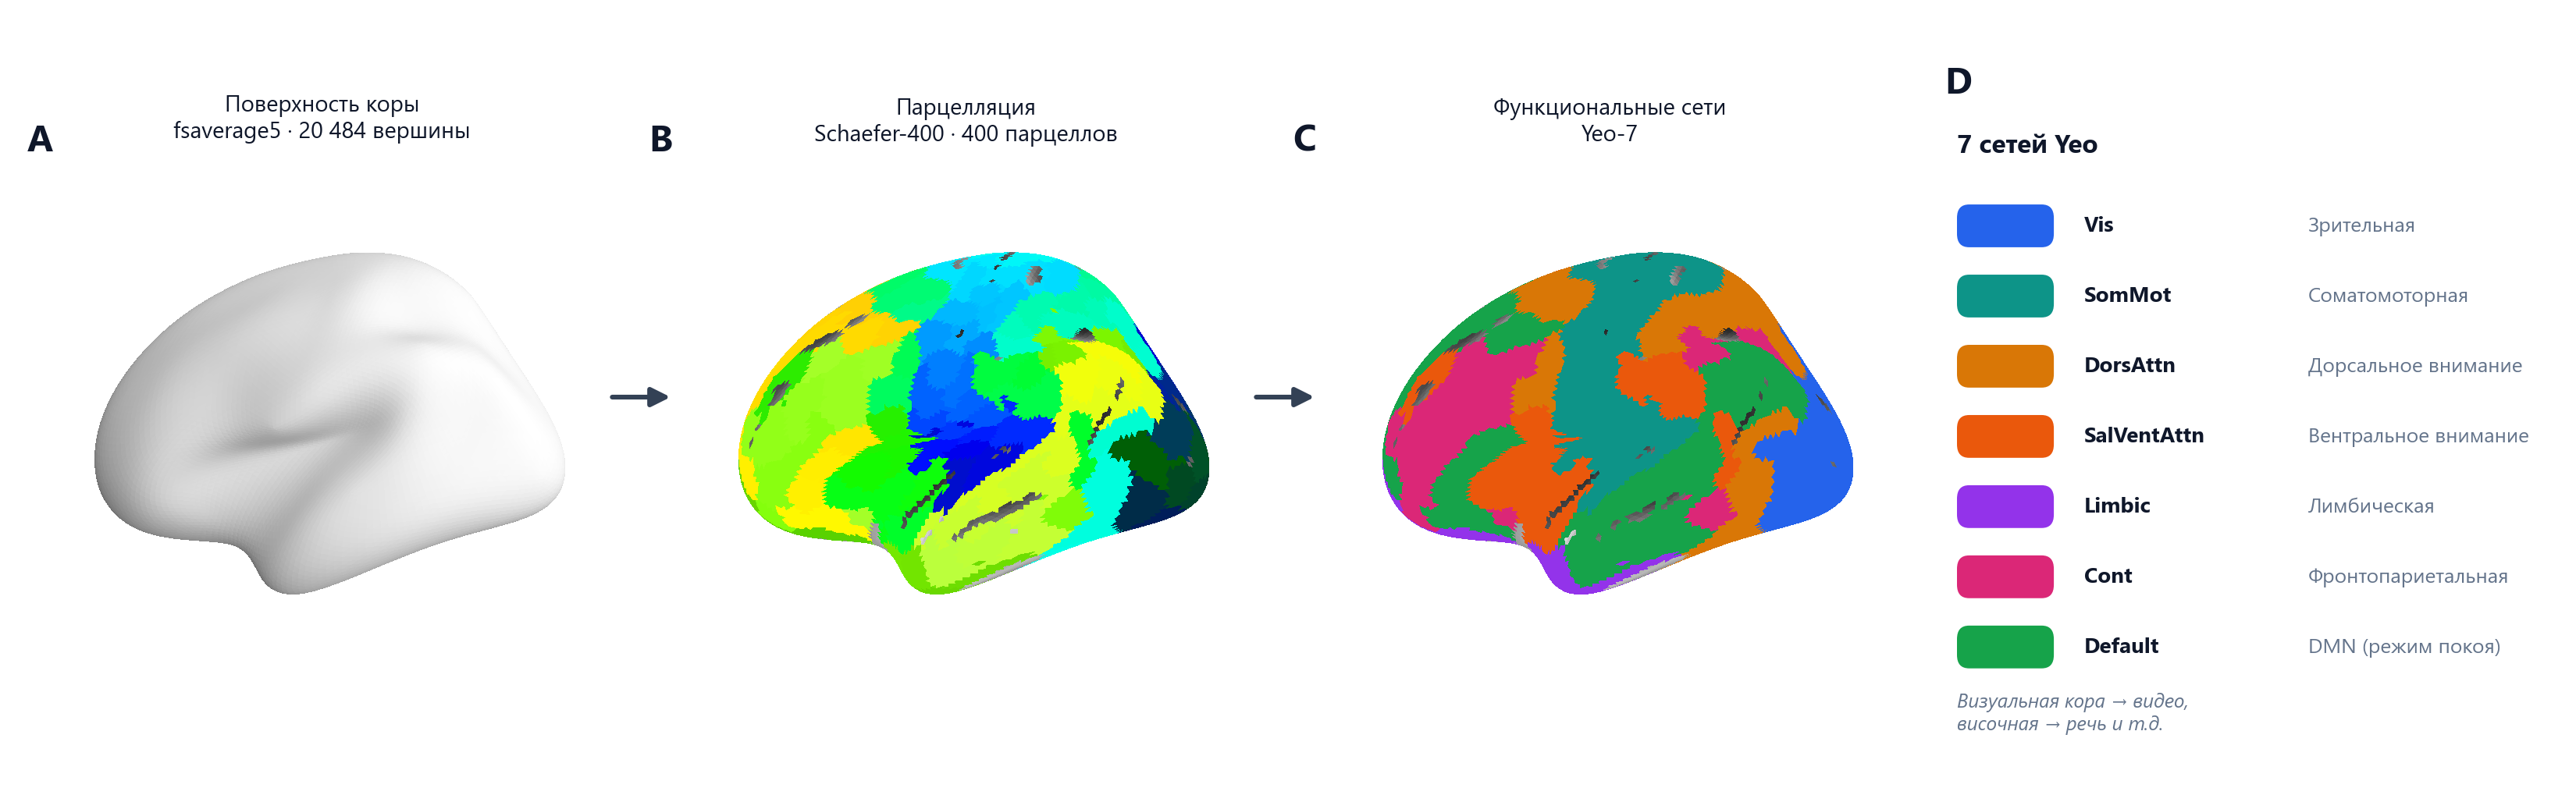
\includegraphics[width=0.98\textwidth]{assets/fig_hierarchy.png}
\caption{Иерархия представления коры: от целостного мозга к
поверхности, от поверхности к парцелляции и далее к функциональным
сетям и ролям. Здесь же~--- почему моделирование <<парцеллов>>
достаточно для подавляющего большинства прикладных задач.}
\label{fig:hierarchy}
\end{figure}

\subsection{Физика фМРТ: BOLD-сигнал как косвенный показатель нейронной активности}
\label{sec:neuro-fmri}

Функциональная МРТ измеряет не сами потенциалы действия нейронов, а
\emph{оксигенацию крови}, называемую BOLD (Blood-Oxygen-Level-Dependent)
сигналом. Физический механизм таков~\cite{Logothetis2008,Buxton1998}:

\begin{enumerate}[label=(\arabic*), leftmargin=*]
    \item При активации нейронов локально усиливается кровоток (нейроваскулярное
          сопряжение, neurovascular coupling).
    \item Усиленный кровоток приносит больше оксигемоглобина
          (диамагнетика) и вымывает дезоксигемоглобин
          (парамагнетик).
    \item Соотношение окси-/дезоксигемоглобина изменяет локальную
          магнитную восприимчивость, что проявляется как усиление
          МРТ-сигнала ($T_2^*$-взвешенный сигнал).
\end{enumerate}

Таким образом, BOLD-сигнал~--- это \emph{опосредованный} показатель
нейронной активности, и между нервным импульсом и наблюдаемым
сигналом проходит несколько секунд. Это ключевое ограничение~---
и одновременно ценная индуктивная предпосылка для моделей
кодирования.

\subsection{Гемодинамическая функция отклика (HRF)}
\label{sec:neuro-hrf}

Связь между коротким стимулом и BOLD-сигналом описывается
\emph{гемодинамической функцией отклика} (HRF, haemodynamic response
function). Каноническая HRF~--- двойной гамма-импульс~\cite{Glover1999,Lindquist2019}:

\begin{equation}
h(t) = \gamma(t; a_1, b_1) - c \cdot \gamma(t; a_2, b_2),
\qquad
\gamma(t; a, b) = \frac{t^{a-1} e^{-t/b}}{b^{a} \Gamma(a)},
\label{eq:hrf-canonical}
\end{equation}
с типичными параметрами $a_1 = 6,\; b_1 = 1,\; a_2 = 16,\;
b_2 = 1,\; c = 1/6$. Здесь $\Gamma$~--- гамма-функция. Пик
HRF приходится примерно на $5$--$6$~секунд после начала
стимула; постстимульное падение (undershoot) приходится на
$15$--$18$~секунд.

Следствия для моделей кодирования:

\begin{itemize}[leftmargin=*]
    \item \textbf{Задержка.} Стимул, наблюдаемый в момент $t$,
          проявляется в BOLD-ответе не ранее момента $t + 4$~с.
          То есть модель должна явно учитывать ~6-секундный лаг.
    \item \textbf{Затухание.} Вклад далёкого прошлого стимула
          экспоненциально мал; моделирование внимания должно
          отражать это~\cite{Lindquist2019}.
    \item \emph{Региональная изменчивость.} Форма HRF варьирует
          по областям мозга; её можно дообучать на данных.
\end{itemize}

\begin{figure}[H]
\centering
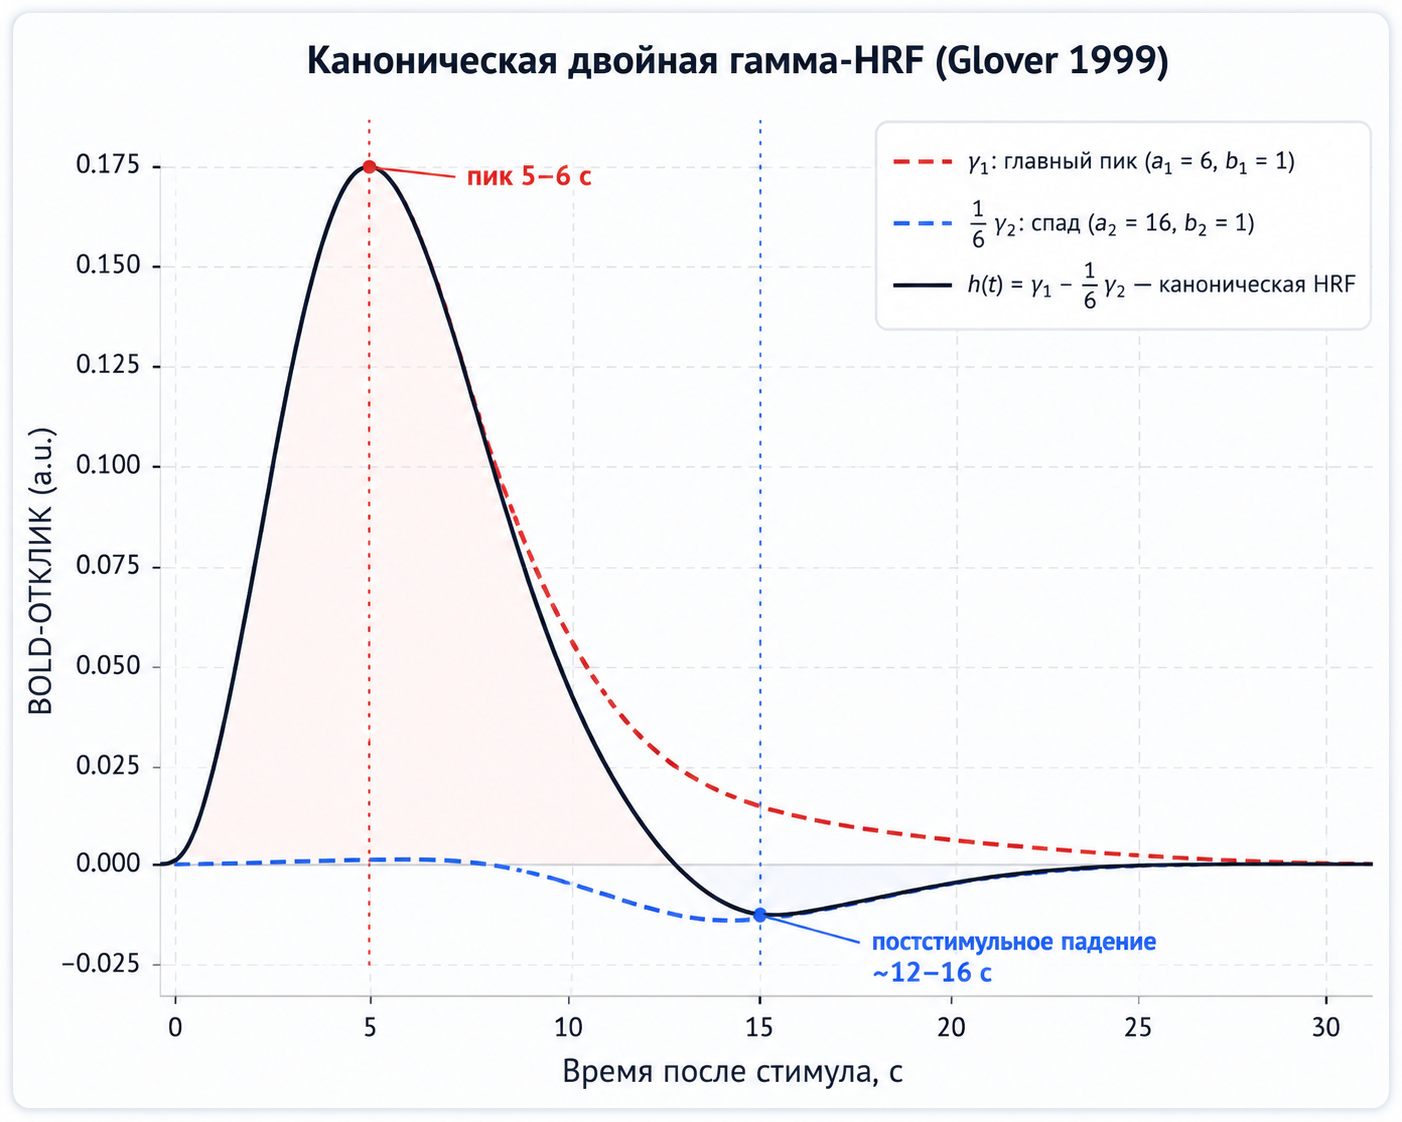
\includegraphics[width=0.8\textwidth]{assets/fig_hrf.png}
\caption{Каноническая двойная гамма-функция гемодинамического
отклика (canonical HRF): суперпозиция положительного
главного пика $\sim$6~с и более медленного отрицательного
постстимульного падения $\sim$16~с, как описано в~\eqref{eq:hrf-canonical}.
Функция играет ключевую роль в индуктивных предпосылках Flora
(\cref{sec:hrf-method}).}
\label{fig:hrf}
\end{figure}

\subsection{<<ФМРТ~--- это очень дорого>>: где именно дорого}
\label{sec:neuro-cost}

Возвращаясь к тезису о дороговизне: дорого \emph{собрать новые данные}.
Стоимость одного субъект-часа фМРТ-исследования варьируется от
$200$~USD (в странах с развитой инфраструктурой) до $1000$~USD и
выше (в академических центрах с оплатой работы операторов и
сопутствующих расходов). Для нейровизуализационного проекта на
$100$ субъектов с шестью часами записей каждый стоимость только
измерений превышает несколько сотен тысяч долларов. Это действительно
делает новые массивы данных дорогими.

Однако для \emph{вычислительной модели} измеренные данные выступают
\emph{эталонной моделью} на этапе обучения, и далее модель работает без
фМРТ-сканера. Открытые нейровизуализационные корпуса
предоставляют готовые обучающие пары <<стимул~--- кортикальный
ответ>>; одна и та же модель может быть обучена и развёрнута в
любой точке мира. Именно в этом состоит переход <<от измерения к
моделированию>>, который реализует Flora.

% ============================================================================
\section{Связанные работы}
\label{sec:related}

\subsection{Классические модели кодирования}
\label{sec:related-encoding}

Линейные модели кодирования (encoding models) на ручных
признаках~\cite{Kay2008} и воксельные модели на глубоких
признаках~\cite{Naselaris2011} положили начало количественному
моделированию того, как зрительная кора отвечает на статические
изображения. Распространение на семантические представления
позволило реконструировать семантические карты
коры~\cite{Mitchell2008,Huth2016,LeBel2023}. Открытый корпус
<<Natural Scenes Dataset>> и Algonauts-челленджи установили стандарт
оценки по попарцеллярной корреляции.

\subsection{Глубокие модели динамического зрения}
\label{sec:related-dynamic}

Свёрточные и рекуррентные модели~\cite{Wen2018} расширили
классические подходы до задачи динамического зрения. Одновременно
появились задачи декодирования: MindEye2~\cite{Scotti2024}
показывает, что мультисубъектное обучение с общим латентным
пространством даёт возможность реконструировать изображение из
фМРТ по часу записей на субъекта.

\subsection{Мультимодальные модели мозга}
\label{sec:related-multimodal}

Современный этап ознаменован тримодальными моделями кодирования
коры на основе замороженных фундаментальных энкодеров
(зрение+язык+аудио). Наиболее заметные результаты
достигнуты в открытом конкурсе Algonauts 2025: модель-победитель
построила единое тримодальное представление, которое обучается
более чем на $1000$~часах фМРТ-записей от $720$~субъектов.
Позже эти результаты были обобщены в масштабной фоновой
модели зрения, слуха и языка~\cite{dAscoli2026tribev2},
показавшей, что единое визуально-аудио-языковое представление
способно кодировать кортикальные ответы на разнообразных наборах.

Flora наследует постановку <<видео+аудио+текст $\rightarrow$
fsaverage5>>, но сознательно работает в \emph{облегчённой
конфигурации}: компактные замороженные энкодеры
($\sim$67~М замороженных параметров против миллиардов) и малый
обучаемый стек ($\sim$10--14~М). Это позволяет проводить все
эксперименты на одной потребительской GPU и открывать модели
для тиражирования.

\subsection{Методологические компоненты}
\label{sec:related-methodology}

В Flora сочетаются четыре линии методов:
\begin{itemize}[leftmargin=*]
    \item \emph{Трансформер}~\cite{Vaswani2017} как ядро мультимодального
          синтеза;
    \item \emph{Mixture-of-Experts} с балансировкой нагрузки и
          z-регуляризацией~\cite{Fedus2022}~--- разреженный
          экспертный блок как замена плотного FFN;
    \item \emph{Перенос знаний между моделями}~\cite{Hinton2015}~--- техника обучения компактной модели
          компактной модели воспроизводить предсказания
          высокоразмерной эталонной модели;
    \item \emph{FiLM-кондиционирование}~\cite{Perez2018}~---
          персубъектная адаптация без посубъектных весовых
          матриц.
\end{itemize}

Энкодеры признаков: MiniLM~\cite{Wang2020}, Whisper~\cite{Radford2023},
MobileViT~\cite{Mehta2022}~--- компактные предобученные модели,
допускающие экспорт в ONNX и квантование.

\subsection{Нейровизуализация, атласы и гемодинамика}
\label{sec:related-neuroimaging}

Поверхностный анализ коры опирается на классические работы
FreeSurfer~\cite{Dale1999,Fischl1999,Fischl2000,Fischl2002,Fischl2012}.
Атлас \textbf{fsaverage5} ($20\,484$~вершины на оба полушария) и
парцелляции Schaefer-400~\cite{Schaefer2018} с разбиением по сетям
Yeo-7~\cite{Yeo2011} образуют стандартную инфраструктуру
поверхностного моделирования. Каноническая двойная гамма-HRF и
методы её моделирования описаны в~\cite{Glover1999,Lindquist2019}.
В качестве программной инфраструктуры мы используем
nilearn~\cite{Abraham2014}.

% ============================================================================
\section{Данные и предобработка}
\label{sec:data}

\subsection{Исходный набор CineBrain}
\label{sec:cinebrain}

Исходным источником служит набор \textbf{CineBrain}~\cite{Gao2025cinebrain,Gao2025cinebrain}~---
первый крупномасштабный корпус синхронных записей фМРТ и ЭЭГ при
аудиовизуальном нарративном стимулировании. Участники слушали и
смотрели эпизоды сериала <<Теория большого взрыва>> в сканере.
Демография и дизайн эксперимента сведены в~\cref{tab:cohort}.

\begin{table}[H]
\centering
\caption{Когорта и дизайн эксперимента CineBrain (по~\cite{Gao2025cinebrain}).}
\label{tab:cohort}
\small
\begin{tabular}{ll}
\toprule
Параметр & Значение \\
\midrule
Участники & 6 (2~муж.\ / 4~жен.) \\
Возраст & 21--26 лет \\
Зрение и слух & норма или скорректированная норма \\
Стимулы & 20~эпизодов <<Теории большого взрыва>> по 18~мин \\
Сезоны & S07 (все); S09 (субъекты 1, 2, 6); S11 (остальные) \\
Объём на участника & 20~ранов $\approx$ 6~ч; $\approx$27\,000 кадров фМРТ \\
Синхронная ЭЭГ & 64~канала, 1000~Гц (в данной работе не используется) \\
Сканер & 3~Т, 32-канальная РЧ-катушка \\
\bottomrule
\end{tabular}
\end{table}

\subsection{МРТ-протокол и предобработка сигнала}
\label{sec:preproc}

Структурные T1-изображения получены последовательностью MPRAGE
($0{,}8$~мм изотропно, TR~$=2500$~мс, TE~$=2{,}22$~мс, угол~$8^\circ$);
функциональные данные~--- градиентно-эхо EPI с полномозговым покрытием
($2$~мм изотропно, TR~$=800$~мс, TE~$=37$~мс, угол~$52^\circ$,
multiband~$=8$; частота дискретизации $1{,}25$~Гц, $1350$~кадров на
ран)~\cite{Gao2025cinebrain}. Предобработка выполнена конвейером
fMRIPrep~\cite{Esteban2019}. Для компенсации гемодинамической задержки
сигналы фМРТ z-нормировались внутри рана со сдвигом $4$~с относительно
стимула~\cite{Gao2025cinebrain}. В исходной работе выделялись зрительная
($8\,405$~вокселей) и слуховая ($10\,541$~воксель) области интереса.

\subsection{Поверхностное представление коры}
\label{sec:surface}

Все кортикальные цели и визуализации Flora работают в поверхностном
пространстве \textbf{fsaverage5} ($20\,484$~вершины)~--- атласе,
исторически построенном инструментарием
FreeSurfer~\cite{Dale1999,Fischl1999,Fischl2002,Fischl2012}.
Объёмные карты проецируются на пиальную/инфлированную поверхность
через \texttt{nilearn.surface.vol\_to\_surf}~\cite{Abraham2014};
обучение ведётся в парцелляции \textbf{Schaefer-400}~\cite{Schaefer2018}
с группировкой по $7$~сетям Yeo~\cite{Yeo2011}. Отображение
$20\,484 \rightarrow 400$ выполняется усреднением вершин внутри
парцеллы (в коде~--- чанковое усреднение
\textsuperscript{\textdagger}).

\begin{figure}[H]
\centering
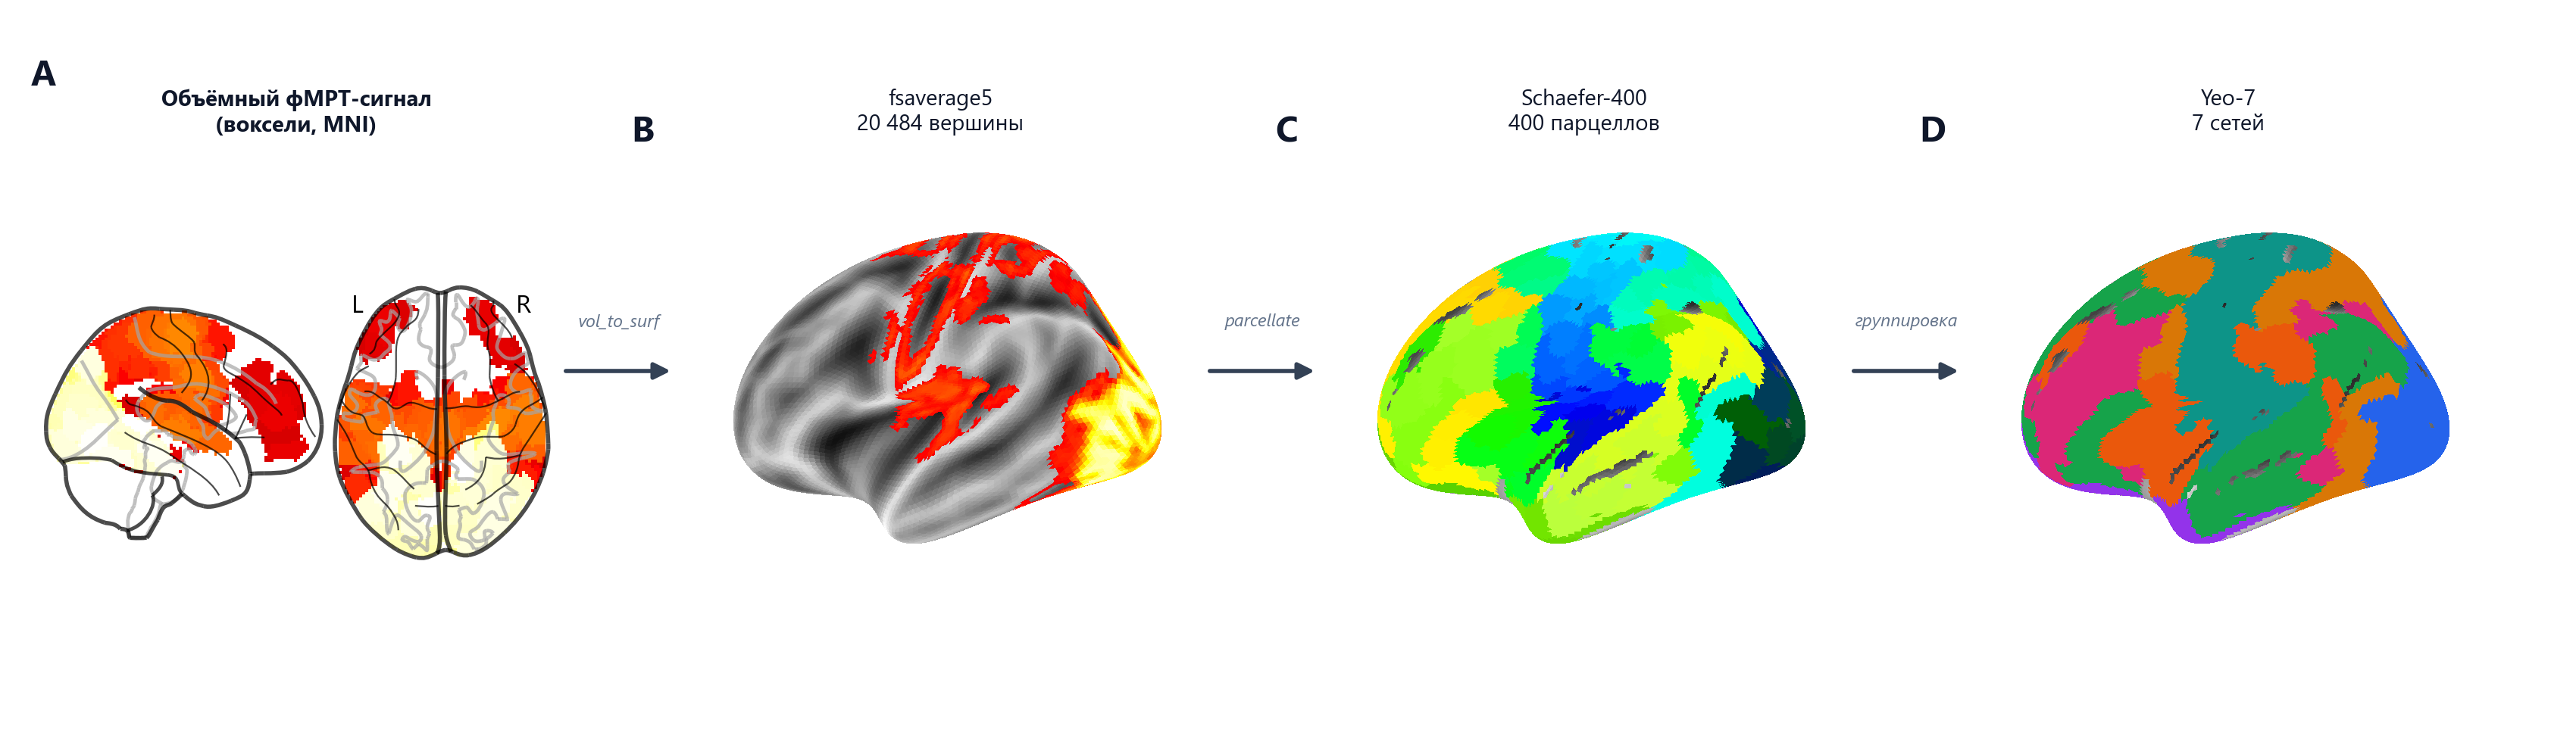
\includegraphics[width=0.99\textwidth]{assets/fig_projection.png}
\caption{Цепочка проекций от объёмного МРТ-сигнала к
функциональным сетям. Все преобразования реализованы в коде
проекта (\texttt{flora/v3\_dataset.py}).}
\label{fig:projection}
\end{figure}

\subsection{Корпус воспроизведения эталонной модели}
\label{sec:corpus}

Обучающий корпус~--- $200$~видеоклипов набора CINE
Brain~\cite{CINEBrain,Gao2025cinebrain}, снабжённых эталонными
предсказаниями кортикальной активности (\texttt{preds.npy},
$20\,484$~вершины fsaverage5); принятое в проекте время
повторения фМРТ~--- TR~$=1{,}5$~с. Разбиение:
\textbf{160~клипов обучение / 40~клипов валидация} (фиксированный
seed~$=42$, доля $0{,}2$). Из каждого клипа скриптом
\texttt{flora/extract\_features\_v3.py} извлекается $T=5$ временных
шагов; файл признаков содержит поля по~\cref{tab:ptformat}.
В локальном архиве \texttt{data/features.zip}~--- ровно $200$~таких
файлов.

\begin{table}[H]
\centering
\caption{Формат одного .pt-файла признаков (из кода
\texttt{extract\_features\_v3.py} и \texttt{train\_lightning.py}).}
\label{tab:ptformat}
\small
\begin{tabular}{llll}
\toprule
Поле & Размерность & Тип & Источник \\
\midrule
\texttt{text}   & $(T, 384)$   & fp16 & all-MiniLM-L6-v2 (нули при отсутствии речи) \\
\texttt{audio}  & $(T, 384)$   & fp16 & энкодер Whisper-Tiny, 16~кГц \\
\texttt{video}  & $(T, 640)$   & fp16 & MobileViT-S, равномерно $T$ кадров \\
\texttt{reference}& $(T, 20484)$ & fp16 & эталонные предсказания (fsaverage5) \\
\texttt{subject\_id} & скаляр & int & идентификатор субъекта (0) \\
\bottomrule
\end{tabular}
\end{table}

\textsuperscript{\textdagger}\,Замечание о границах конвейера: структурный
конвейер FreeSurfer (recon-all: сегментация, измерение толщины
коры, атласная разметка) в самом проекте Flora не запускается~---
используются готовые поверхности fsaverage5 из nilearn. Точное
атласное отображение fsaverage5 $\rightarrow$ Schaefer-400
(\texttt{.annot}) реализовано чанковым усреднением, что
задокументировано в коде как \emph{placeholder} для дальнейшего
уточнения (см. список пробелов в~\cref{app:gaps}).

% ============================================================================
\section{Метод}
\label{sec:method}

\subsection{Обзор архитектуры}
\label{sec:arch}

Flora отображает три потока стимула~--- видео (2~кадра/с), аудио
(16~кГц) и транскрипт~--- во временной ряд кортикальной
активности (\cref{fig:overview,fig:arch}). Конструкция следует
принципу <<замороженное восприятие, обучаемый синтез>>: обучаются
только проекторы, трансформер синтеза, HRF-свёртка и выходная
голова.

\begin{figure}[H]
\centering
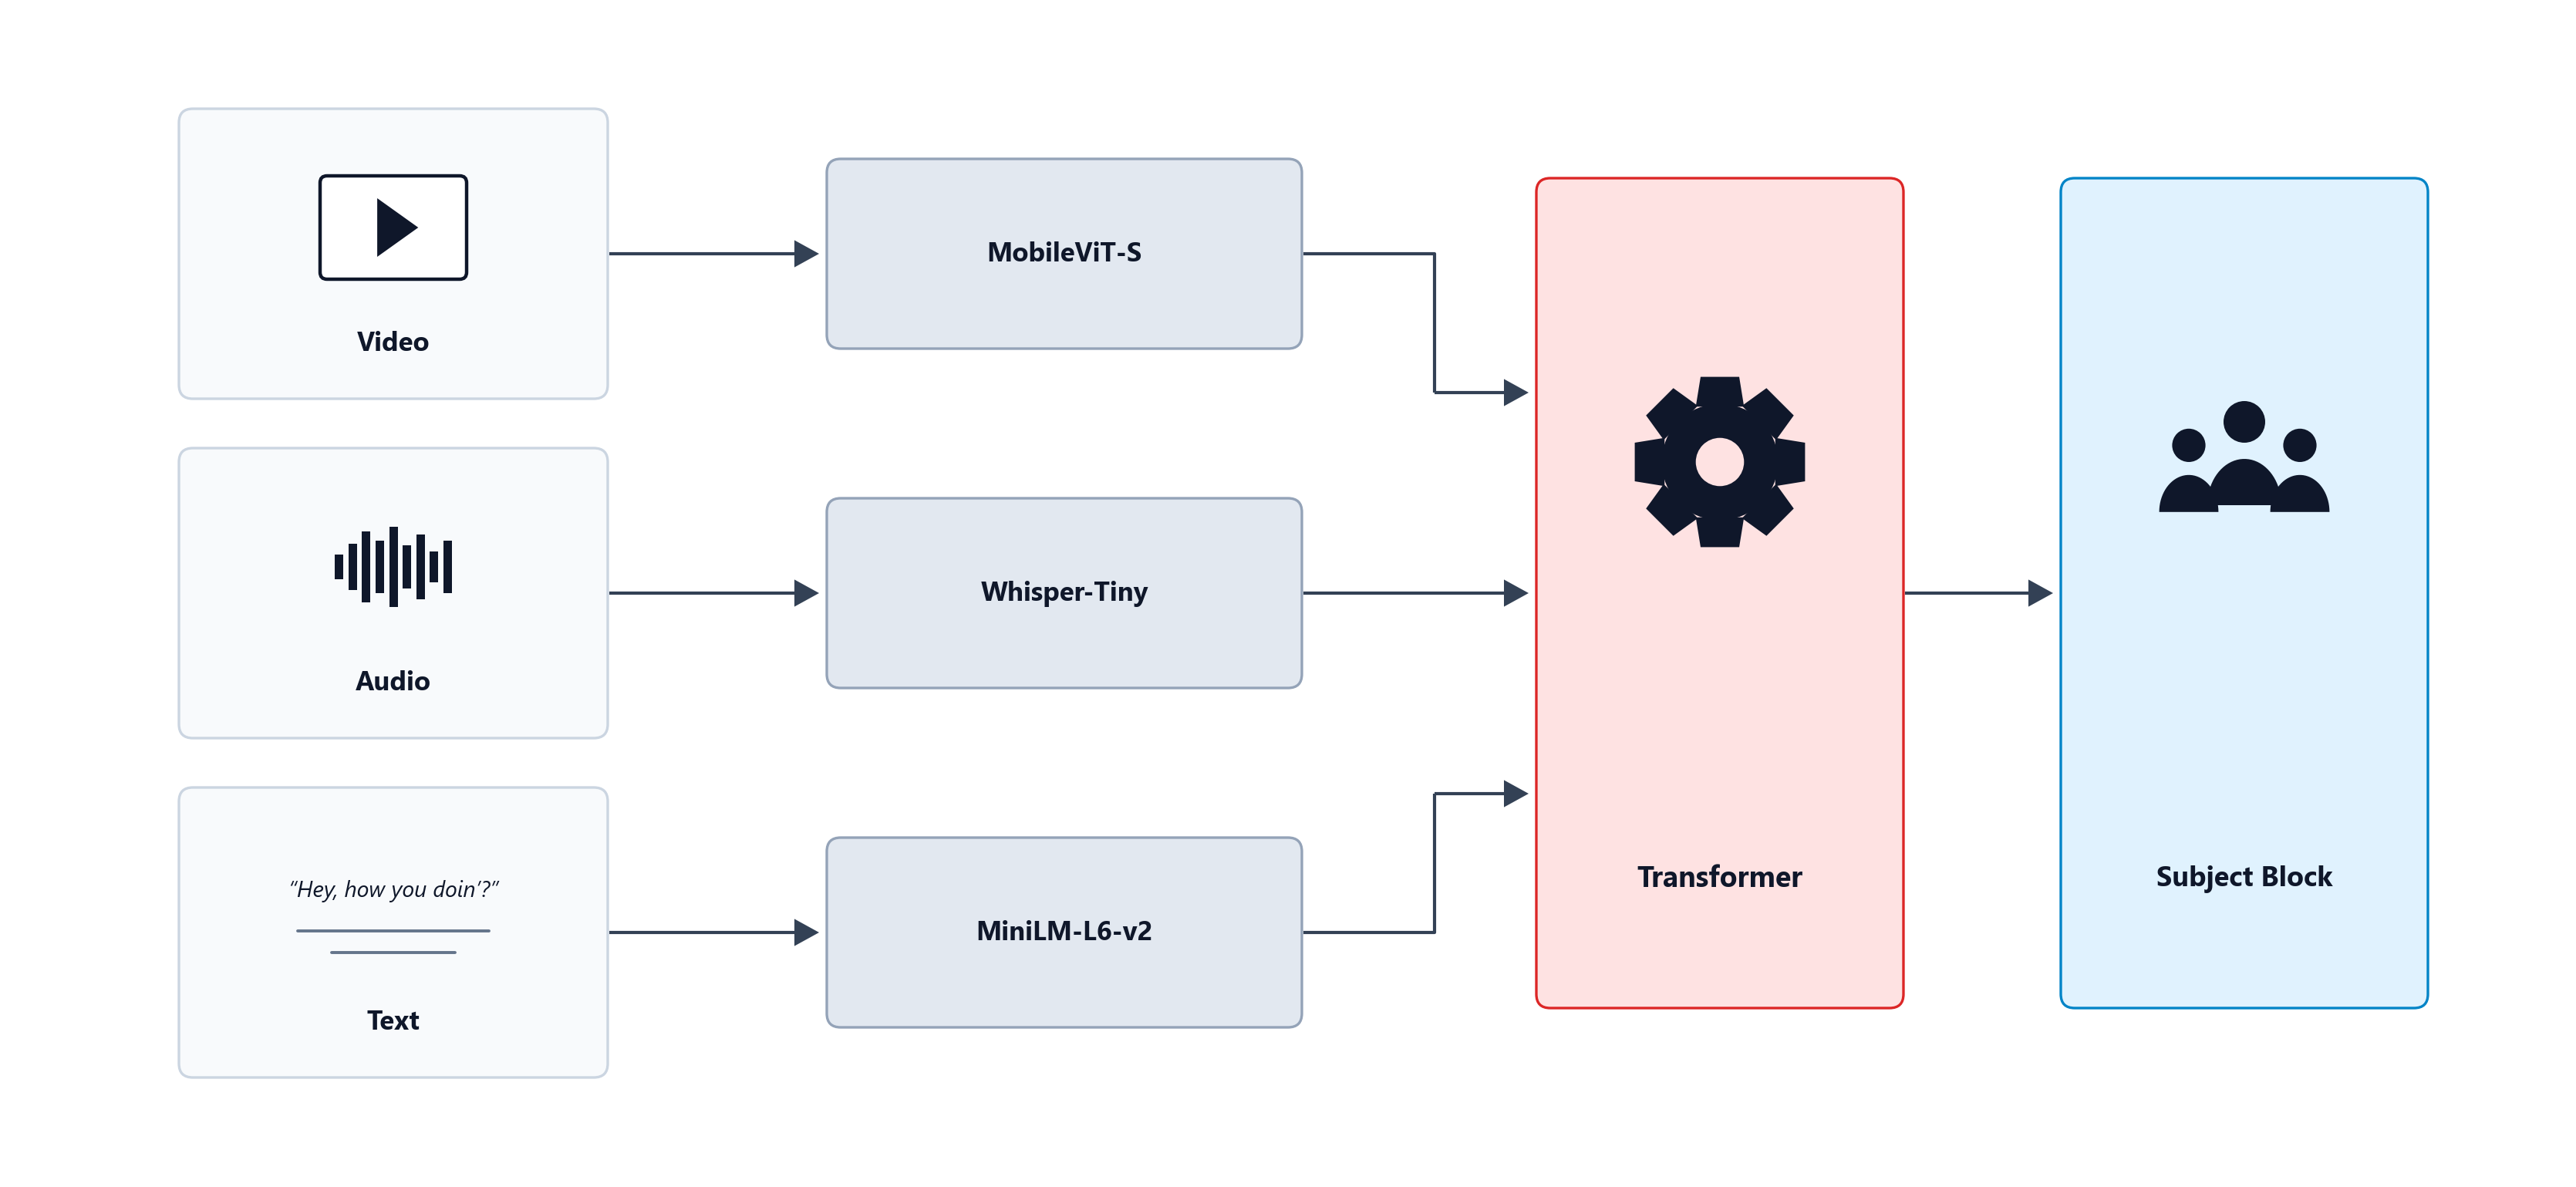
\includegraphics[width=0.98\textwidth]{assets/flora_architecture.png}
\caption{Архитектура Flora: три модальности стимула проходят через
замороженные энкодеры (MobileViT-S, Whisper-Tiny, MiniLM-L6-v2),
объединяются трансформером синтеза и преобразуются блоком субъекта
в кортикальное предсказание (фигура проекта:
\texttt{assets/flora\_architecture.png}).}
\label{fig:arch}
\end{figure}

\subsection{Замороженные модальные энкодеры}
\label{sec:encoders}

Для каждой модальности $m \in \{v, a, \ell\}$ замороженный энкодер
строит эпизодический эмбеддинг:
\begin{equation}
z_m(t) = \mathrm{Enc}_m\!\big(x_m(t)\big), \qquad
z_m(t) \in \mathbb{R}^{d_m}, \quad d_v = 640,\; d_a = d_\ell = 384,
\label{eq:features}
\end{equation}
где $x_v$~--- кадры видео, $x_a$~--- лог-мел спектрограмма,
$x_\ell$~--- токены транскрипта. Энкодеры и их размерности
перечислены в~\cref{tab:encoders}; суммарный замороженный
бюджет~--- $67{,}3$~млн параметров.

\begin{table}[H]
\centering
\caption{Замороженные энкодеры признаков (из \texttt{flora/config.py}).}
\label{tab:encoders}
\small
\begin{tabular}{llcc}
\toprule
Модальность & Энкодер & Выход & Параметры \\
\midrule
Текст  & all-MiniLM-L6-v2~\cite{Wang2020}  & 384 & 22{,}7~млн \\
Аудио  & энкодер Whisper-Tiny~\cite{Radford2023} & 384 & 39~млн \\
Видео  & MobileViT-S~\cite{Mehta2022} & 640 & 5{,}6~млн \\
\midrule
\multicolumn{2}{l}{\textbf{Итого (заморожено)}} & & \textbf{67{,}3~млн} \\
\bottomrule
\end{tabular}
\end{table}

\subsection{Модальные проекторы и модуль движения}
\label{sec:projectors}

Каждый поток проецируется в общее пространство $\mathbb{R}^{D}$,
$D = 512$, трёхслойным MLP с промежуточной размерностью $768$
(LayerNorm $\rightarrow$ Linear $\rightarrow$ GELU $\rightarrow$
Dropout $\rightarrow$ Linear $\rightarrow$ GELU $\rightarrow$
Dropout $\rightarrow$ Linear $\rightarrow$ LayerNorm):
\begin{equation}
h_m(t) = P_m\big(z_m(t)\big) \in \mathbb{R}^{D}.
\label{eq:projector}
\end{equation}
Поскольку MobileViT-S~--- покадровый энкодер, к видеопотоку
добавляется глубинная каузальная временная свёртка (ядро~$3$),
инициализированная конечной разностью $[-\tfrac{1}{2}, 0, \tfrac{1}{2}]$:
\begin{equation}
\tilde{h}_v(t) = h_v(t) + \big(\mathrm{DWConv1D}_{k=3}\, h_v\big)(t),
\label{eq:motion}
\end{equation}
что резидуально добавляет сигнал межкадрового движения, критичный
для motion-чувствительной коры (MT+/V5).

\begin{figure}[H]
\centering
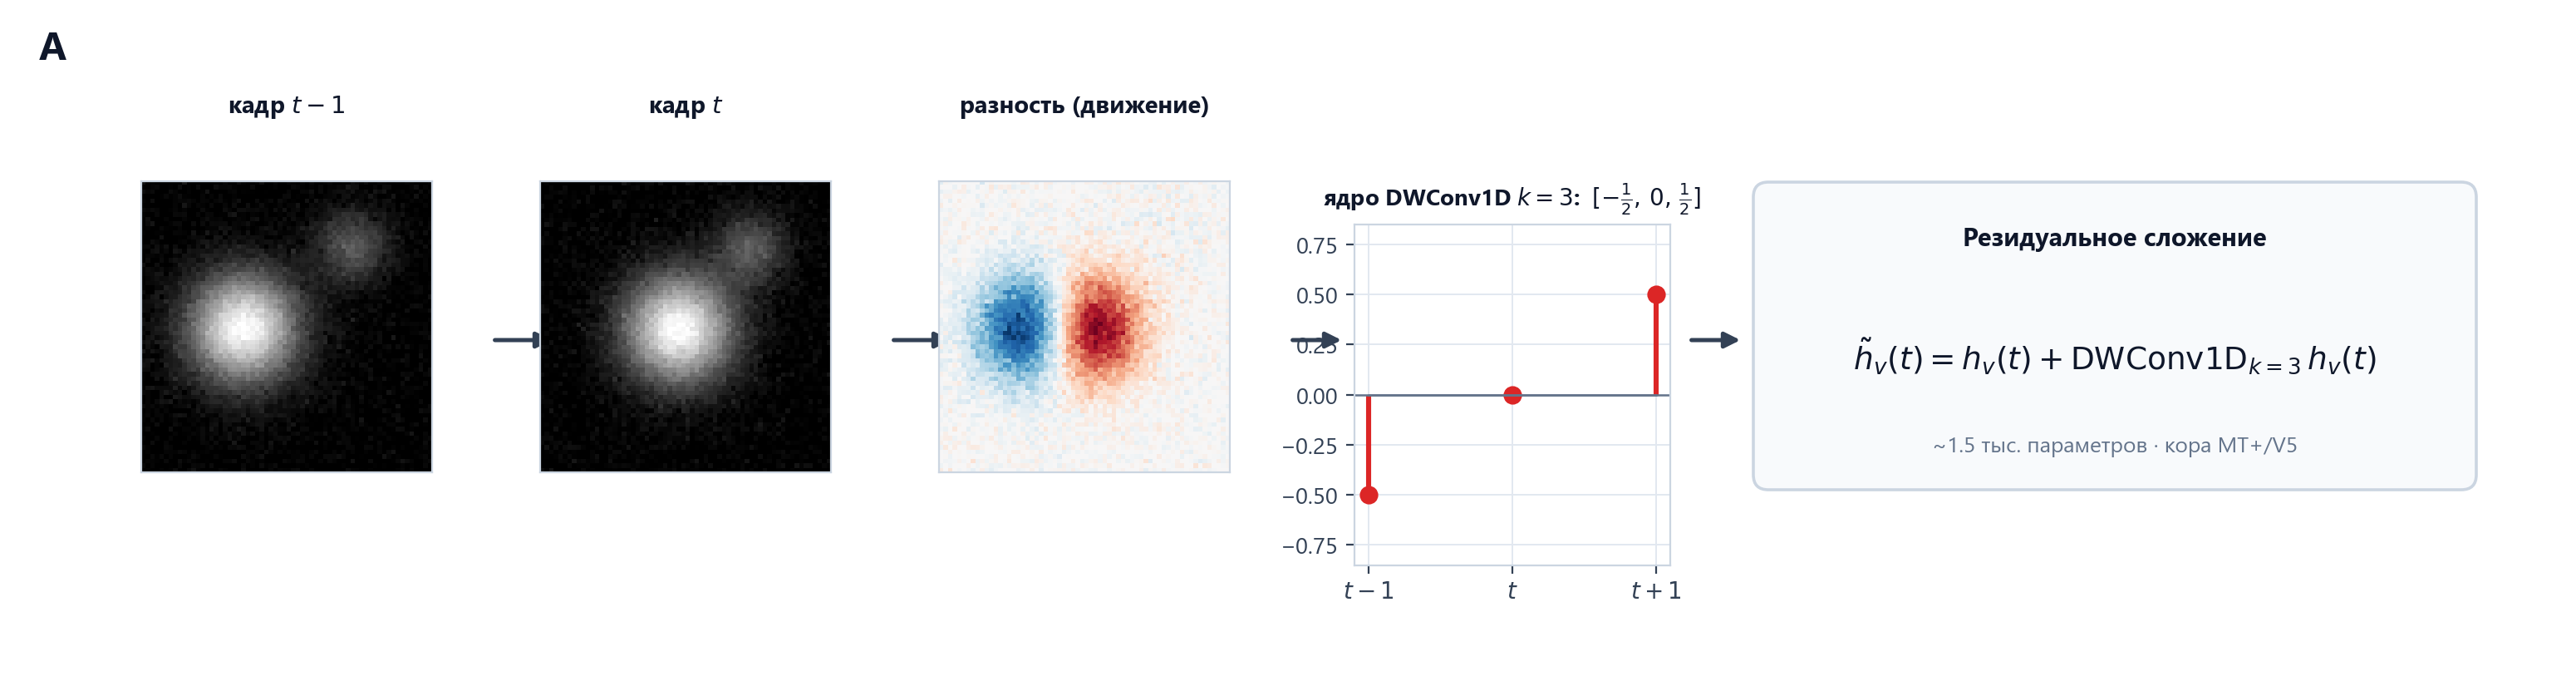
\includegraphics[width=0.95\textwidth]{assets/fig_motion.png}
\caption{Модуль движения \texttt{TemporalMotionModule}:
к покадровому MobileViT-S добавляется сигнал межкадровой
разности ($\approx 1{,}5$~тыс. параметров).}
\label{fig:motion}
\end{figure}

\subsection{Токенизация времени и интерливинг}
\label{sec:tokenization}

К каждому токену добавляются обучаемый модальный эмбеддинг $e_m$
и помодальный временной эмбеддинг $e^{\mathrm{time}}_m(\tau)$; три
потока перемежаются в единую последовательность
\begin{equation}
u = [\,v_1, a_1, \ell_1, v_2, a_2, \ell_2, \dots\,] \in
\mathbb{R}^{3T \times D}, \qquad u \leftarrow u + p_{1:3T},
\label{eq:interleave}
\end{equation}
где $p$~--- общий обучаемый позиционный эмбеддинг. Интерливинг
делает кросс-модальное внимание внутри одного шага времени
доступным уже с первого слоя.

\subsection{MoE-трансформер с HRF-затухающим смещением внимания}
\label{sec:moe}

Трансформер синтеза состоит из $L = 4$ pre-norm
блоков~\cite{Vaswani2017} ($8$~голов, $ff\_mult = 2$). В \emph{первых
двух} слоях к логитам внимания добавляется обучаемое гемодинамическое
смещение, отражающее доминирование недавней истории стимула в
текущем BOLD-ответе:
\begin{equation}
\mathrm{Attn}(Q, K, V) = \mathrm{softmax}\!\left(
\frac{QK^{\top}}{\sqrt{d_k}} + B \right) V, \qquad
B_{ij} = -\alpha\,|\Delta \tau_{ij}|,
\label{eq:hrfbias}
\end{equation}
где $\Delta \tau_{ij}$~--- расстояние между токенами в единицах TR
($3$~токена на TR), $\alpha$~--- обучаемый послойный параметр
затухания, инициализированный так, что вес на расстоянии $6$~TR
равен $0{,}5$. Два верхних слоя~--- полное внимание для нарративной
семантической интеграции.

\begin{figure}[H]
\centering
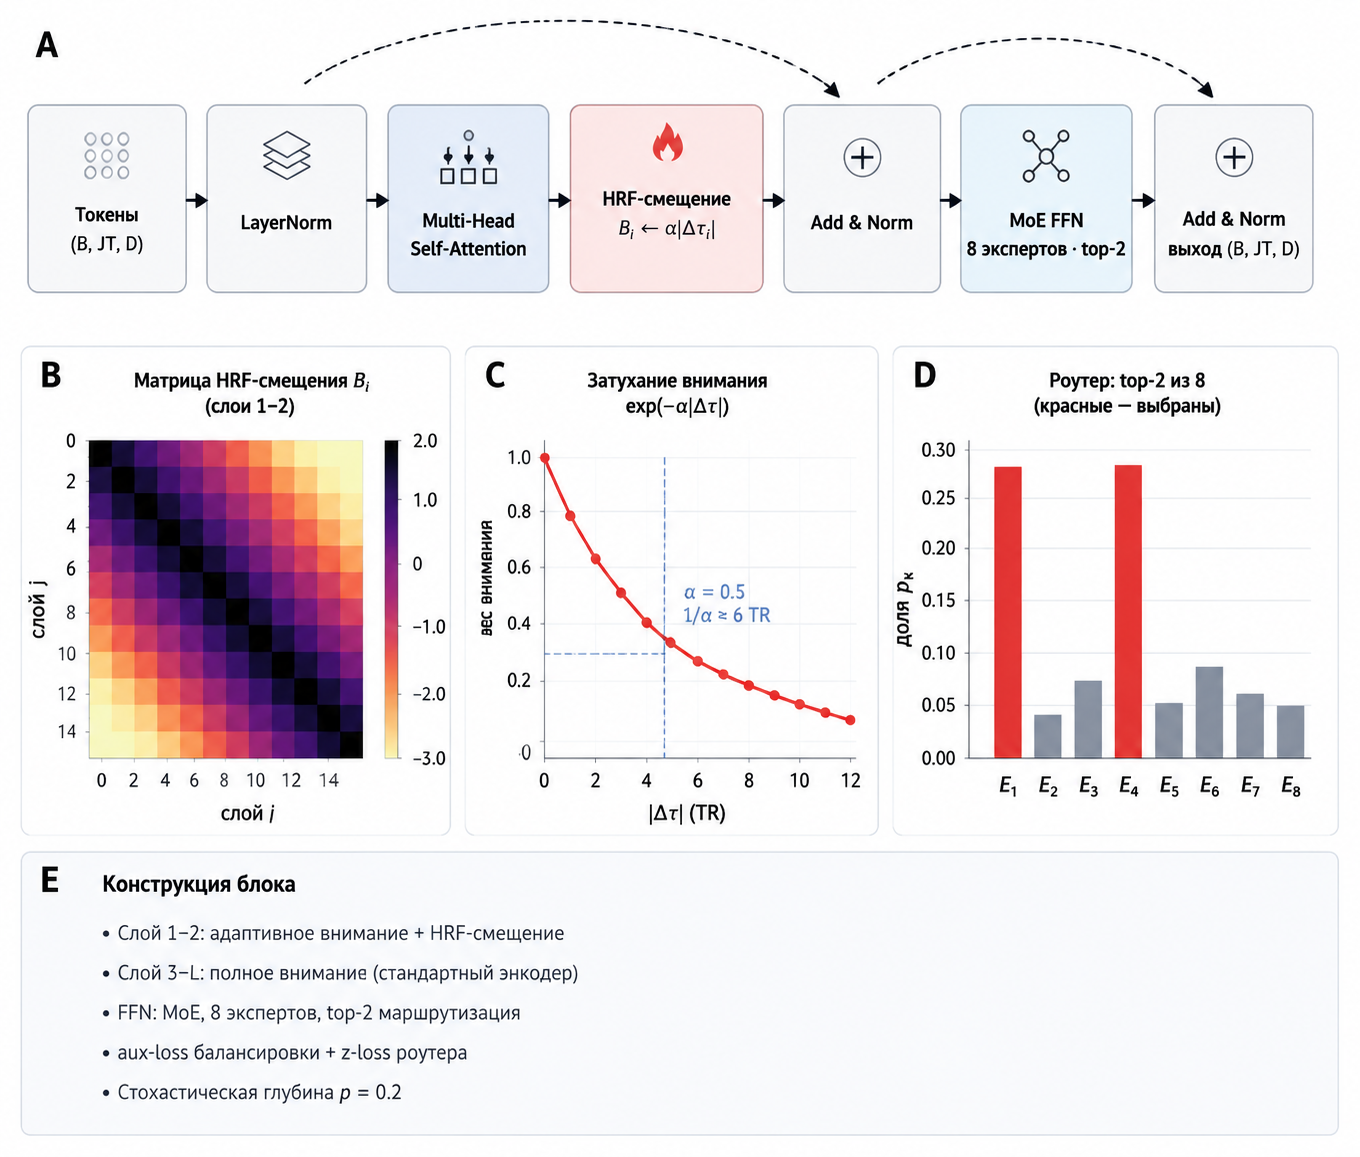
\includegraphics[width=0.98\textwidth]{assets/fig_moe_block.png}
\caption{Блок MoE-трансформера: pre-norm, локальный
self-attention с HRF-затухающим смещением внимания (в слоях
1--2), полный self-attention (слои 3--4), затем FFN-смесь
экспертов (8 экспертов, top-2 маршрутизация,
балансировочный aux-loss и z-loss роутера). Вход и выход
связаны резидуально.}
\label{fig:moe-block}
\end{figure}

\begin{figure}[H]
\centering
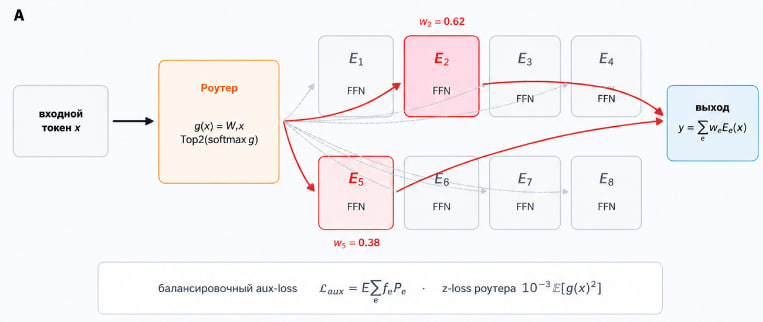
\includegraphics[width=0.92\textwidth]{assets/fig_moe_router.png}
\caption{Маршрутизация Mixture-of-Experts: входной токен
$x$ направляется роутером $\mathrm{Top2}(g(x))$ ровно в двух из
$E=8$ экспертов; их выходы смешиваются согласно softmax-весам.
Балансировочный aux-loss ($N \sum_e f_e P_e$) и z-loss
штрафуют неравномерную загрузку и большие логиты соответственно.}
\label{fig:moe-router}
\end{figure}

Каждый FFN-блок~--- смесь из $E = 8$ экспертов с маршрутизацией
top-$2$~\cite{Fedus2022}:
\begin{equation}
y(x) = \sum_{e \in \mathrm{Top2}(g(x))}
\frac{\exp g_e(x)}{\sum_{e' \in \mathrm{Top2}} \exp g_{e'}(x)}\,
E_e(x),
\label{eq:moe}
\end{equation}
где $g(x)$~--- линейный роутер, $E_e$~--- двухслойный FFN-эксперт.
Эксперты инициализируются из общего базового FFN с малым шумом
$\sigma = 0{,}01$, что предотвращает коллапс маршрутизации.
Обучение стабилизируется двумя регуляризаторами: балансировочной
потерей в стиле Switch Transformer
\begin{equation}
\mathcal{L}_{\mathrm{aux}} = E \sum_{e=1}^{E} f_e P_e,
\label{eq:aux}
\end{equation}
где $f_e$~--- доля токенов, направленных эксперту~$e$, $P_e$~---
средняя вероятность роутера; и z-потерей роутера
\begin{equation}
\mathcal{L}_{z} = 10^{-3}\,\mathbb{E}\!\left[\, g(x)^2 \,\right],
\label{eq:zloss}
\end{equation}
штрафующей большие логиты. Глубина регуляризуется стохастической
глубиной с линейным расписанием $0 \rightarrow 0{,}2$ (более
глубокие слои пропускаются чаще).

\subsection{Гейтованное объединение модальностей}
\label{sec:gating}

Вместо усреднения трёх модальных токенов шага времени обучаются
мягкие гейты (softmax по модальностям; инициализация нулями даёт
стартовое равномерное взвешивание $1/3$):
\begin{equation}
g(t) = \mathrm{softmax}\big(W_g\, \bar{h}(t) + b_g\big) \in
\mathbb{R}^{3}, \qquad
\hat{h}(t) = \sum_{m \in \{v,a,\ell\}} g_m(t)\, h_m(t),
\label{eq:gating}
\end{equation}
где $\bar{h}(t)$~--- среднее модальных токенов. Это позволяет
разным кортикальным системам взвешивать модальности согласно их
функциональной роли (зрительная кора~--- видео, речевая~--- текст).

\begin{figure}[H]
\centering
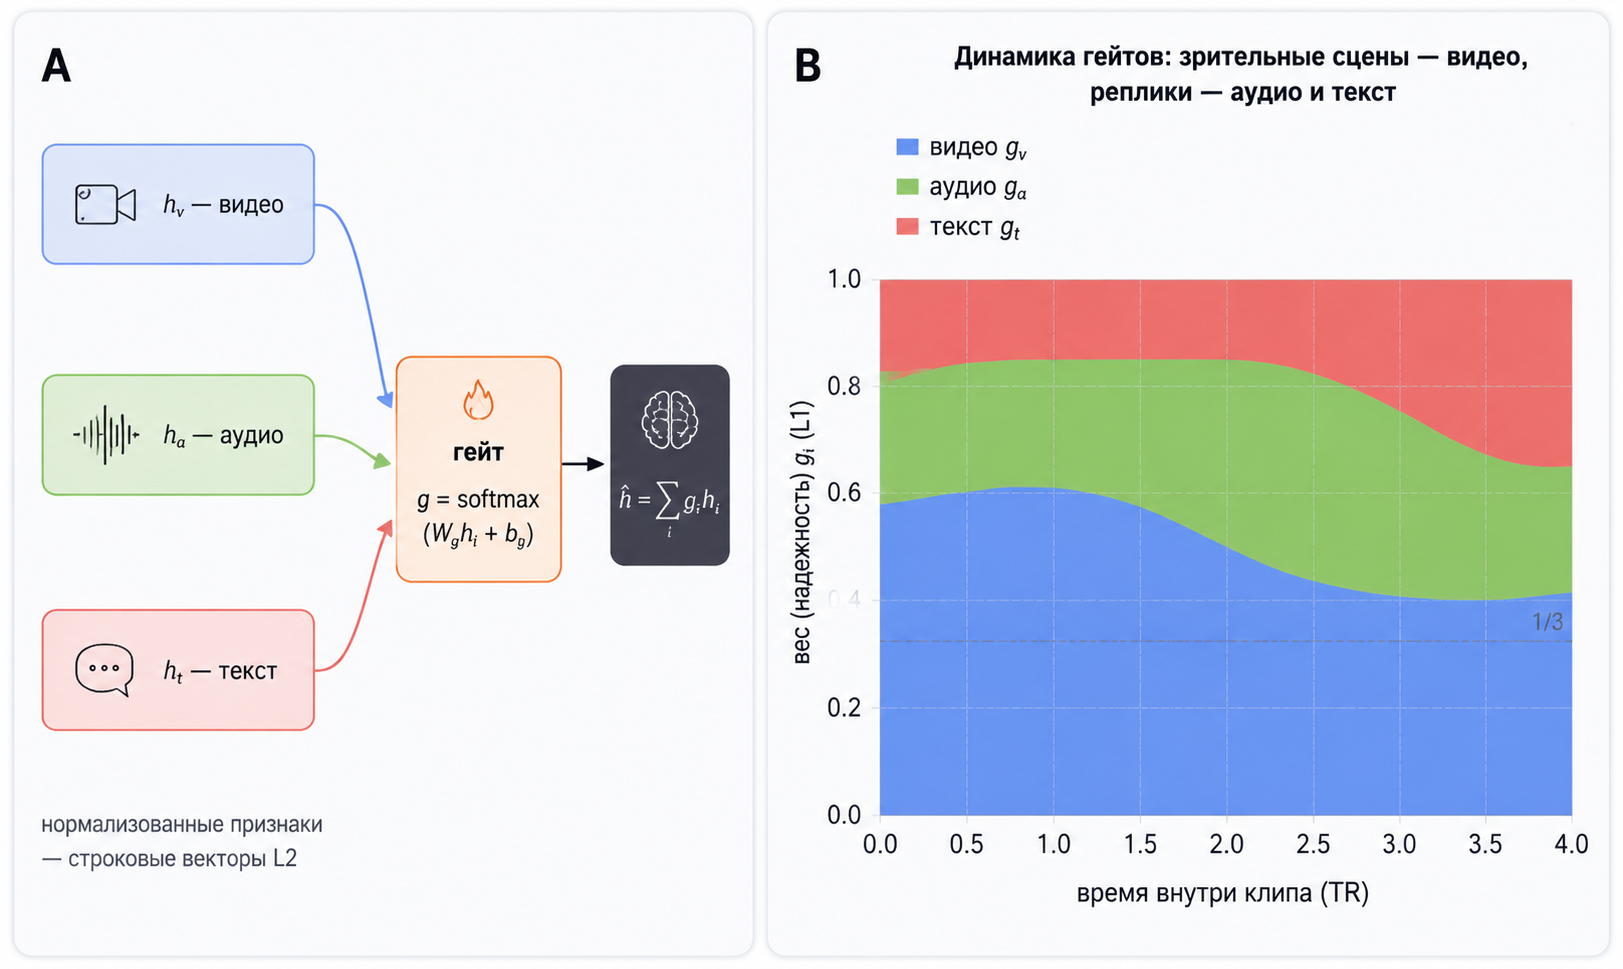
\includegraphics[width=0.94\textwidth]{assets/fig_gating.png}
\caption{Гейтованное объединение модальностей: вместо
безусловного среднего три модальных токена смешиваются с
обучаемыми per-timestep весами $g(t) \in \mathbb{R}^3$,
инициализированными равномерно $1/3$.}
\label{fig:gating-fig}
\end{figure}

\subsection{Гемодинамическая свёртка}
\label{sec:hrf-method}

Синтезированная последовательность проходит каузальную глубинную
свёртку (ядро~$8$~TR, $\approx 12$~с при TR~$=1{,}5$~с),
инициализированную каноническим двойным
гамма-HRF~\cite{Glover1999,Lindquist2019}:
\begin{equation}
h(\tau) = \gamma(\tau;\, a_1{=}6, b_1{=}1)
\;-\; \tfrac{1}{6}\,\gamma(\tau;\, a_2{=}16, b_2{=}1), \qquad
\gamma(\tau; a, b) = \frac{\tau^{a-1} e^{-\tau/b}}{b^{a}\,\Gamma(a)},
\label{eq:hrf}
\end{equation}
на сетке $\tau \in \{0, 1{,}5, \dots, 10{,}5\}$~с; ядро нормируется
по $L_1$ и дообучается совместно с моделью (резидуальная ветвь
сохраняет исходный сигнал). Таким образом задержка пика $\sim$6~с и
постстимульное падение $\sim$12--16~с встроены в архитектуру как
априорное знание (\cref{fig:hrf}).

\subsection{Выходная голова с FiLM-кондиционированием}
\label{sec:film}

Общий MLP сопровождается посубъектным FiLM-преобразованием~\cite{Perez2018}
и линейной проекцией в пространство парцеллов:
\begin{equation}
y_s = \gamma_s \odot x + \beta_s, \qquad
\hat{y}_s = W_{\mathrm{out}}\, y_s \in \mathbb{R}^{400 \times T},
\label{eq:film}
\end{equation}
где $\gamma_s, \beta_s \in \mathbb{R}^{D}$~--- эмбеддинги субъекта~$s$
(инициализация~--- тождественное преобразование: $\gamma = 1$,
$\beta = 0$). FiLM заменяет посубъектные весовые матрицы: при
$S = 25$ субъектах и $D = 512$ это $25\,600$ параметров вместо
$\approx 32{,}8$~млн. Выход при необходимости децимируется
адаптивным средним пулингом до целевого числа TR; $400$ парцеллярных
рядов разворачиваются на поверхность fsaverage5 для оценки и рендера.

\begin{figure}[H]
\centering
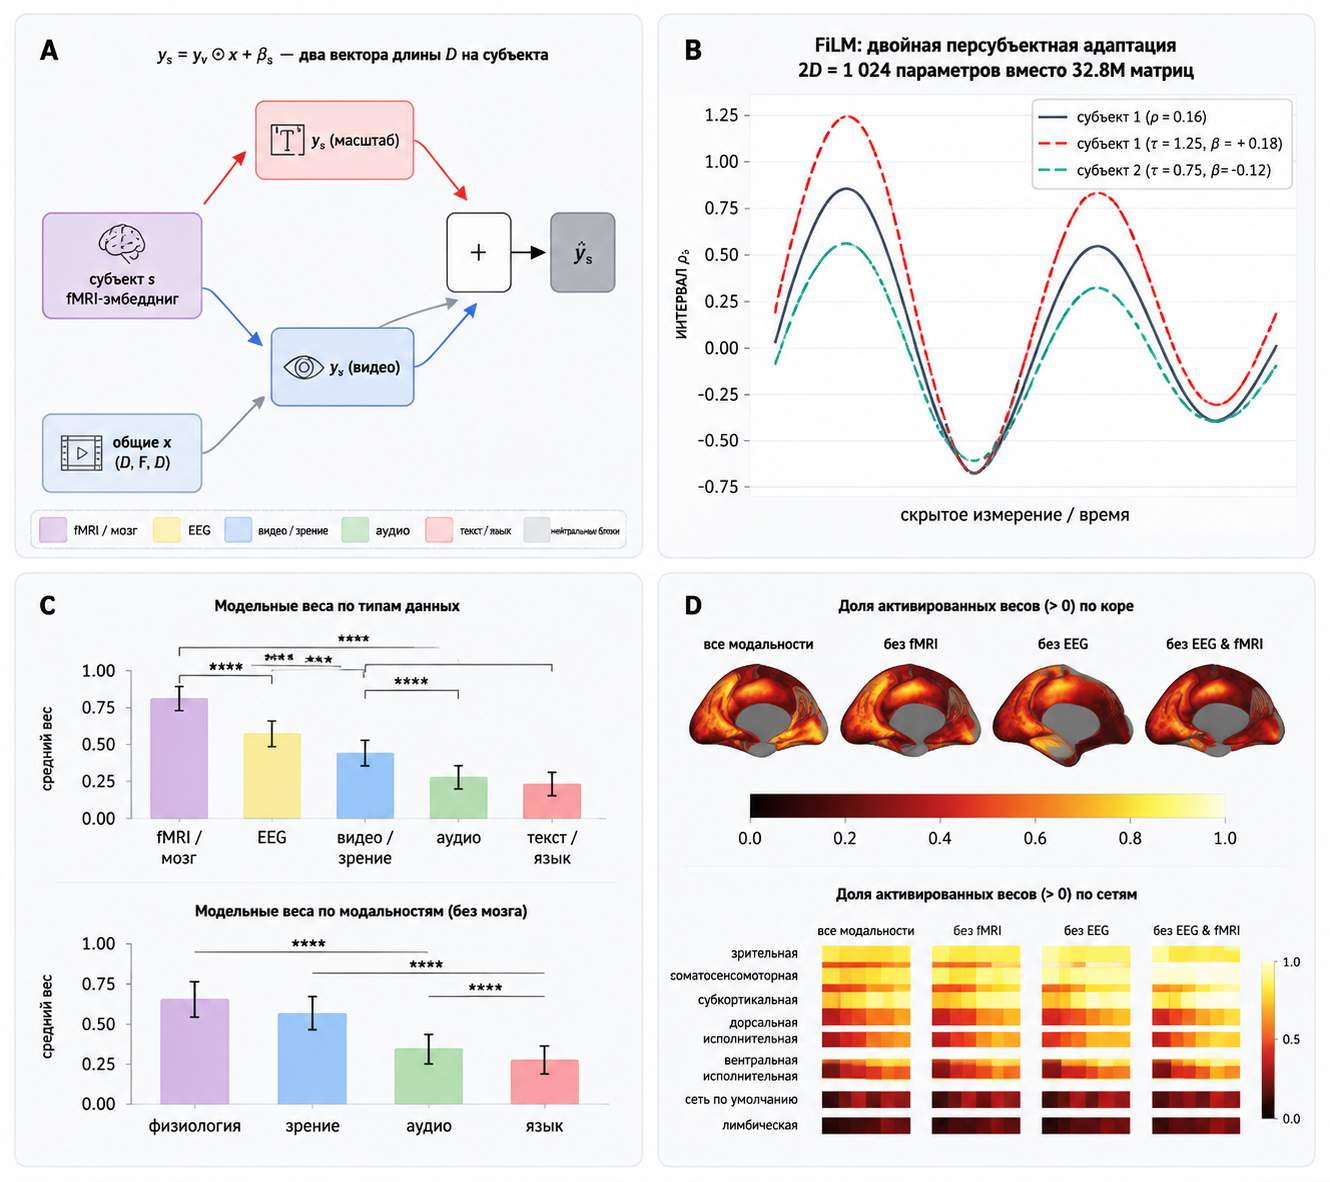
\includegraphics[width=0.94\textwidth]{assets/fig_film.png}
\caption{FiLM-кондиционирование: персубъектные векторы
$\gamma_s$ и $\beta_s$ масштабируют и сдвигают общее
представление $x$. Вместо посубъектных весовых матриц~---
два вектора длины $D$.}
\label{fig:film-fig}
\end{figure}

\subsection{Функции потерь и метрика}
\label{sec:losses}

\subsubsection{Целевая функция воспроизведения эталона}
\label{sec:loss-kd}

В основном эксперименте модель учится воспроизводить эталонные
предсказания кортикальных ответов, доставшиеся от большой
фоновой модели. По коду \texttt{flora/train\_lightning.py}:
\begin{equation}
\mathcal{L}_{\mathrm{KD}} =
0{,}60\,\underbrace{\mathrm{MSE}(\hat{y}, y^{\mathrm{ref}})}_{\text{выход}}
+ 0{,}10\,\underbrace{\mathbb{E}\big[(\hat{y}_{t} - \hat{y}_{t-1})^2\big]}_{\text{временная когерентность}}
+ 0{,}05\,\underbrace{\mathrm{MSE}\big(\hat{y}_{::2}, y^{\mathrm{ref}}_{::2}\big)}_{\text{мультиразрешение}}
+ 0{,}01\,\mathcal{L}_{\mathrm{aux}},
\label{eq:kdtotal}
\end{equation}
где $\hat{y}_{::2}$~--- децимация по времени с шагом~$2$.

\subsubsection{Метрика качества}

Метрика качества~--- средняя попарцеллярная корреляция Пирсона
между предсказанием и целью на отложенной выборке:
\begin{equation}
r_v = \frac{\sum_i (\hat{y}_{v,i} - \bar{\hat{y}}_v)
(y_{v,i} - \bar{y}_v)}
{\sqrt{\sum_i (\hat{y}_{v,i} - \bar{\hat{y}}_v)^2}\,
 \sqrt{\sum_i (y_{v,i} - \bar{y}_v)^2}}, \qquad
r = \frac{1}{V} \sum_{v=1}^{V} r_v,
\label{eq:pearson}
\end{equation}
где индекс~$i$ пробегает все пары (клип, TR) валидационной выборки,
$V = 400$ парцеллов.

\subsubsection{Расширенный режим}

Предусмотрены фазы: самоконтролируемый претрейнинг (Phase~$1$),
уточнение с feature-KD по косинусной близости скрытых представлений
(Phase~$2$: веса $0{,}6/0{,}2/0{,}1/0{,}05/0{,}01$) и файнтюнинг на
реальном фМРТ-сигнале (Phase~$3$) с комбинированной потерей
\begin{equation}
\mathcal{L}_{\mathrm{fMRI}} = 0{,}40\,\big(\tfrac{1}{2}(1 - r)
+ \tfrac{1}{2}\mathrm{MSE}\big) + 0{,}30\,\mathcal{L}_{\mathrm{ref}}
+ 0{,}10\,\mathcal{L}_{\mathrm{feat}} + 0{,}10\,\mathcal{L}_{\mathrm{temp}}
+ 0{,}01\,\mathcal{L}_{\mathrm{aux}}.
\label{eq:fmriloss}
\end{equation}
Результаты фаз 1 и 3 в настоящем репозитории не зафиксированы
(\cref{app:gaps}).

\subsection{Прямой проход пошагово}
\label{sec:forward}

\begin{enumerate}[label=\textbf{\arabic*.}, leftmargin=*, itemsep=1pt]
    \item Замороженные энкодеры строят $z_v, z_a, z_\ell$
          (\cref{eq:features}).
    \item Проекторы переводят каждый поток в $\mathbb{R}^{512}$
          (\cref{eq:projector}); к видео добавляется motion-свёртка
          (\cref{eq:motion}).
    \item Добавляются модальные и помодальные временные эмбеддинги;
          потоки перемежаются и получают общий позиционный
          эмбеддинг (\cref{eq:interleave}).
    \item \emph{(Только обучение)} модальный dropout обнуляет
          случайные модальности ($p = 0{,}5$ в основном эксперименте),
          всегда оставляя хотя бы одну.
    \item Четыре MoE-блока: слои 1--2 с HRF-смещением
          (\cref{eq:hrfbias}), слои 3--4~--- полное внимание; FFN~---
          top-2 смесь экспертов (\cref{eq:moe}) с потерями
          (\cref{eq:aux},\,\cref{eq:zloss}); стохастическая глубина.
    \item Финальный LayerNorm; гейтованное объединение модальностей
          в один токен на TR (\cref{eq:gating}).
    \item Каузальная HRF-свёртка (\cref{eq:hrf}) моделирует
          гемодинамический отклик.
    \item Output-MLP (GELU) $\rightarrow$ FiLM по субъекту
          (\cref{eq:film}) $\rightarrow$ линейная проекция в $400$
          парцеллов $\rightarrow$ адаптивный пулинг до целевого
          числа TR.
\end{enumerate}

\subsection{Бюджет параметров}
\label{sec:params}

\begin{table}[H]
\centering
\caption{Бюджет обучаемых параметров полной конфигурации (README
проекта) и фактический размер опубликованного чекпоинта POC.}
\label{tab:params}
\small
\begin{tabular}{lcc}
\toprule
Компонент & Полная конфигурация & Чекпоинт POC \\
\midrule
Проекторы + модуль движения        & $\sim$2{,}5~млн & --- \\
MoE-трансформер (4 слоя / 2 слоя)  & $\sim$9~млн     & --- \\
Гейтинг, HRF-свёртка, эмбеддинги   & $\sim$0{,}4~млн & --- \\
Выходная голова + FiLM             & $\sim$2~млн     & --- \\
\midrule
\textbf{Всего обучаемых} & \textbf{$\sim$14~млн} & \textbf{9{,}70~млн} \\
Замороженные энкодеры    & 67{,}3~млн            & 67{,}3~млн \\
\bottomrule
\end{tabular}
\end{table}

Полная конфигурация ($D{=}512$, $4$~слоя, $8$~экспертов) оценивается
в $\sim$14~млн обучаемых параметров; проверенный чекпоинт
\texttt{pearson\_r=0.7278.ckpt} содержит POC-вариант ($D{=}256$,
$2$~слоя, $4$~эксперта, $400$~парцеллов, $1$~субъект)~---
$9{,}70$~млн параметров по фактическому подсчёту в
\texttt{state\_dict} (\cref{fig:budget}).

\begin{figure}[H]
\centering
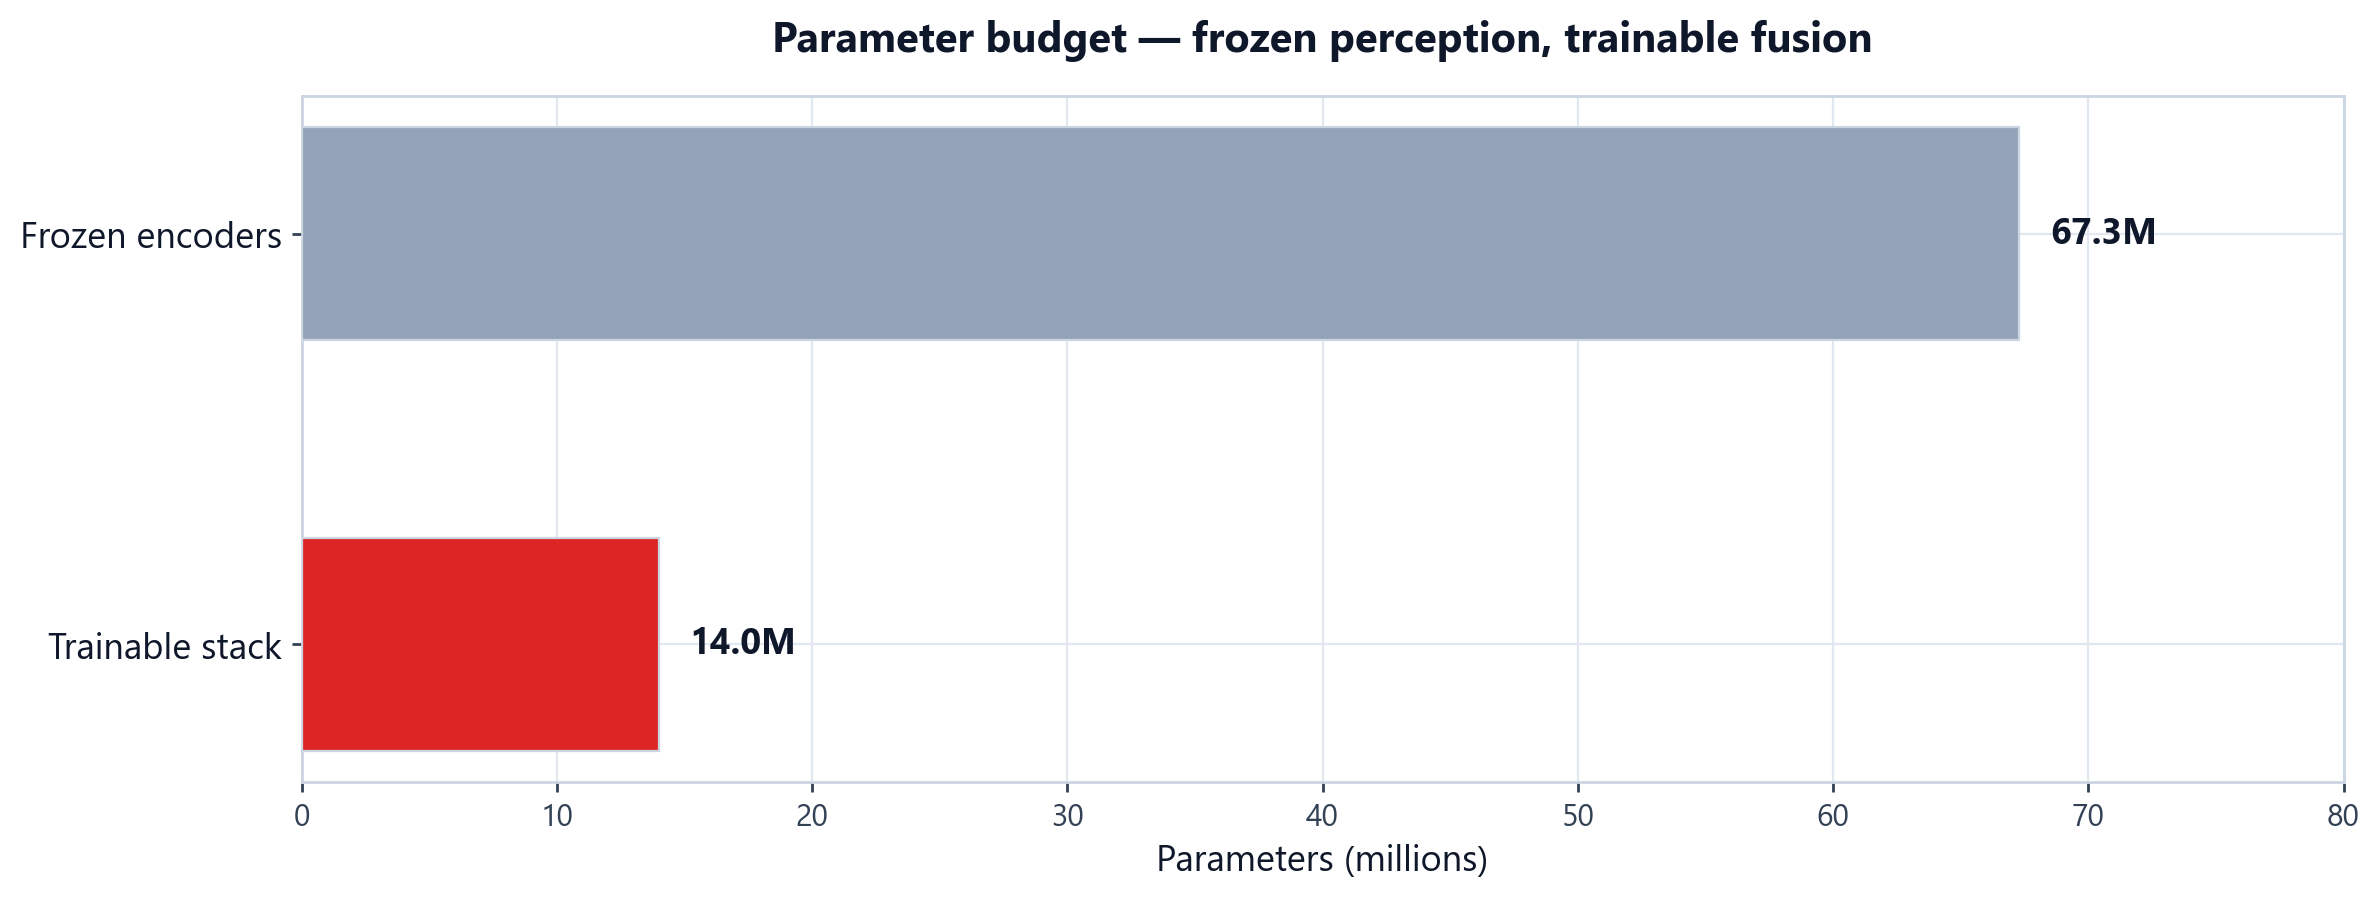
\includegraphics[width=0.9\textwidth]{assets/parameter_budget.png}
\caption{Бюджет параметров: $67{,}3$~млн замороженных параметров
восприятия против $\sim$14~млн обучаемого стека синтеза. Уже
$POC$-вариант при $9{,}7$~млн обучаемых достигает высокого
качества (\texttt{assets/parameter\_budget.png}).}
\label{fig:budget}
\end{figure}

% ============================================================================
\section{Экспериментальная настройка}
\label{sec:setup}

\subsection{Обучение}
\label{sec:training}

Гиперпараметры основного эксперимента извлечены непосредственно
из опубликованного чекпоинта (\texttt{hyper\_parameters}) и кода
\texttt{flora/train\_lightning.py} и сведены в~\cref{tab:hyper}
(полный список~--- в~\cref{app:hyper}). Обучение велось
оптимизатором AdamW~\cite{Loshchilov2019} ($\beta = (0{,}9, 0{,}98)$,
$\varepsilon = 10^{-8}$; weight decay отключён для смещений и
LayerNorm), с линейным прогревом $3$~эпохи и косинусным затуханием,
клиппингом градиента $1{,}0$ и ранней остановкой (patience~$=20$)
по метрике \texttt{val/pearson\_r}.

\begin{table}[H]
\centering
\caption{Ключевые гиперпараметры основного эксперимента (источник:
чекпоинт \texttt{pearson\_r=0.7278.ckpt} и \texttt{train\_lightning.py}).}
\label{tab:hyper}
\small
\begin{tabular}{ll}
\toprule
Параметр & Значение \\
\midrule
Оптимизатор & AdamW, lr $=10^{-3}$, wd $=0{,}1$ \\
Расписание lr & прогрев 3~эпохи $\rightarrow$ косинус \\
Размер батча & 16 \\
Скрытая размерность / слои / головы & 256 / 2 / 4 \\
Эксперты / top-$k$ / ff\_mult & 4 / 2 / 2 \\
Dropout / модальный dropout & 0{,}3 / 0{,}5 \\
Парцеллы / субъекты & 400 (Schaefer-400) / 1 \\
Разбиение & 160 обучение / 40 валидация (seed 42) \\
Ранняя остановка & patience 20, монитор \texttt{val/pearson\_r} \\
Клиппинг градиента & 1{,}0 \\
\bottomrule
\end{tabular}
\end{table}

\subsection{Протокол оценки}
\label{sec:eval}

Метрика (\cref{eq:pearson}) вычисляется на всей валидационной
выборке в конце каждой эпохи: предсказания и цели всех клипов
конкатенируются, корреляция считается по каждой парцелле и
усредняется. Чекпоинты с тремя лучшими значениями сохраняются;
лучшим стал \texttt{checkpoints/best-epoch=052-val/pearson\_r=0.7278.ckpt}
($114$~МБ). Дополнительно код вычисляет стандартное отклонение
$r_v$ и $90$-й процентиль.

\subsection{Базовые модели и абляции}
\label{sec:baselines}

В качестве базовой модели реализован и \emph{запущен} линейный
энкодер в духе классических линейных базлайнов~\cite{Kay2008}:
ridge-регрессия из конкатенированных признаков трёх модальностей
($384 + 384 + 640 = 1408$ признаков на шаг времени) в $400$~парцеллов
($\lambda = 10^{-2}$; $0{,}56$~млн параметров), обученная на тех же
$160$~клипах и оцененная на тех же $40$~отложенных
(\texttt{scripts/benchmark\_flora.py}). Результаты сравнения~--- в
\cref{sec:benchmarks}. Абляции компонентов (HRF-свёртка, MoE,
гейтинг, FiLM) и разреженные варианты архитектуры
(\texttt{flora/v3\_sparse.py}) в репозитории зафиксированы только
кодом, без результатов (\cref{app:gaps}).

% ============================================================================
\section{Результаты}
\label{sec:results}

\subsection{Динамика обучения и итоговая метрика}
\label{sec:main-results}

\begin{table}[H]
\centering
\caption{Реальные метрики проекта (средний попарцеллярный Pearson~$r$
между предсказаниями модели и эталонными ответами на $40$ отложенных
клипах). Источники: README, имя чекпоинта, фактический прогон
\texttt{scripts/benchmark\_flora.py} (2026-08-28).}
\label{tab:results}
\small
\begin{tabular}{lc}
\toprule
Метрика & Значение \\
\midrule
Pearson $r$ на эпохе 0            & 0{,}0328 \\
\textbf{Лучший Pearson $r$ (валидация)} & \textbf{0{,}7278} \\
Лучшая эпоха                      & 52 \\
Pearson $r$ на эпохе 250          & 0{,}6158 \\
\midrule
\multicolumn{2}{l}{\emph{Попарцеллярное распределение (фактический прогон):}} \\
std / p50 / p90                   & 0{,}1640 / 0{,}7590 / 0{,}8916 \\
max / min                         & 0{,}9457 / $-$0{,}3056 \\
\midrule
Обучаемых параметров (чекпоинт)   & 9{,}70~млн \\
Обучающих / валидационных клипов  & 160 / 40 \\
\bottomrule
\end{tabular}
\end{table}

Лучшее значение $r = 0{,}7278$ достигнуто на эпохе~$52$
(\cref{tab:results}); фактический прогон чекпоинта на воспроизведённом
сплите подтверждает это значение с точностью до четвёртого знака
($\bar r = 0{,}72777$). К эпохе $250$ валидационная метрика
снижается до $0{,}6158$ при продолжающемся росте обучающей, что
указывает на переобучение после точки оптимума и мотивирует раннюю
остановку и отбор чекпоинта по валидации (\cref{fig:training}).
Сводная инфографика бенчмарка приведена на \cref{fig:dashboard}.

\begin{figure}[H]
\centering
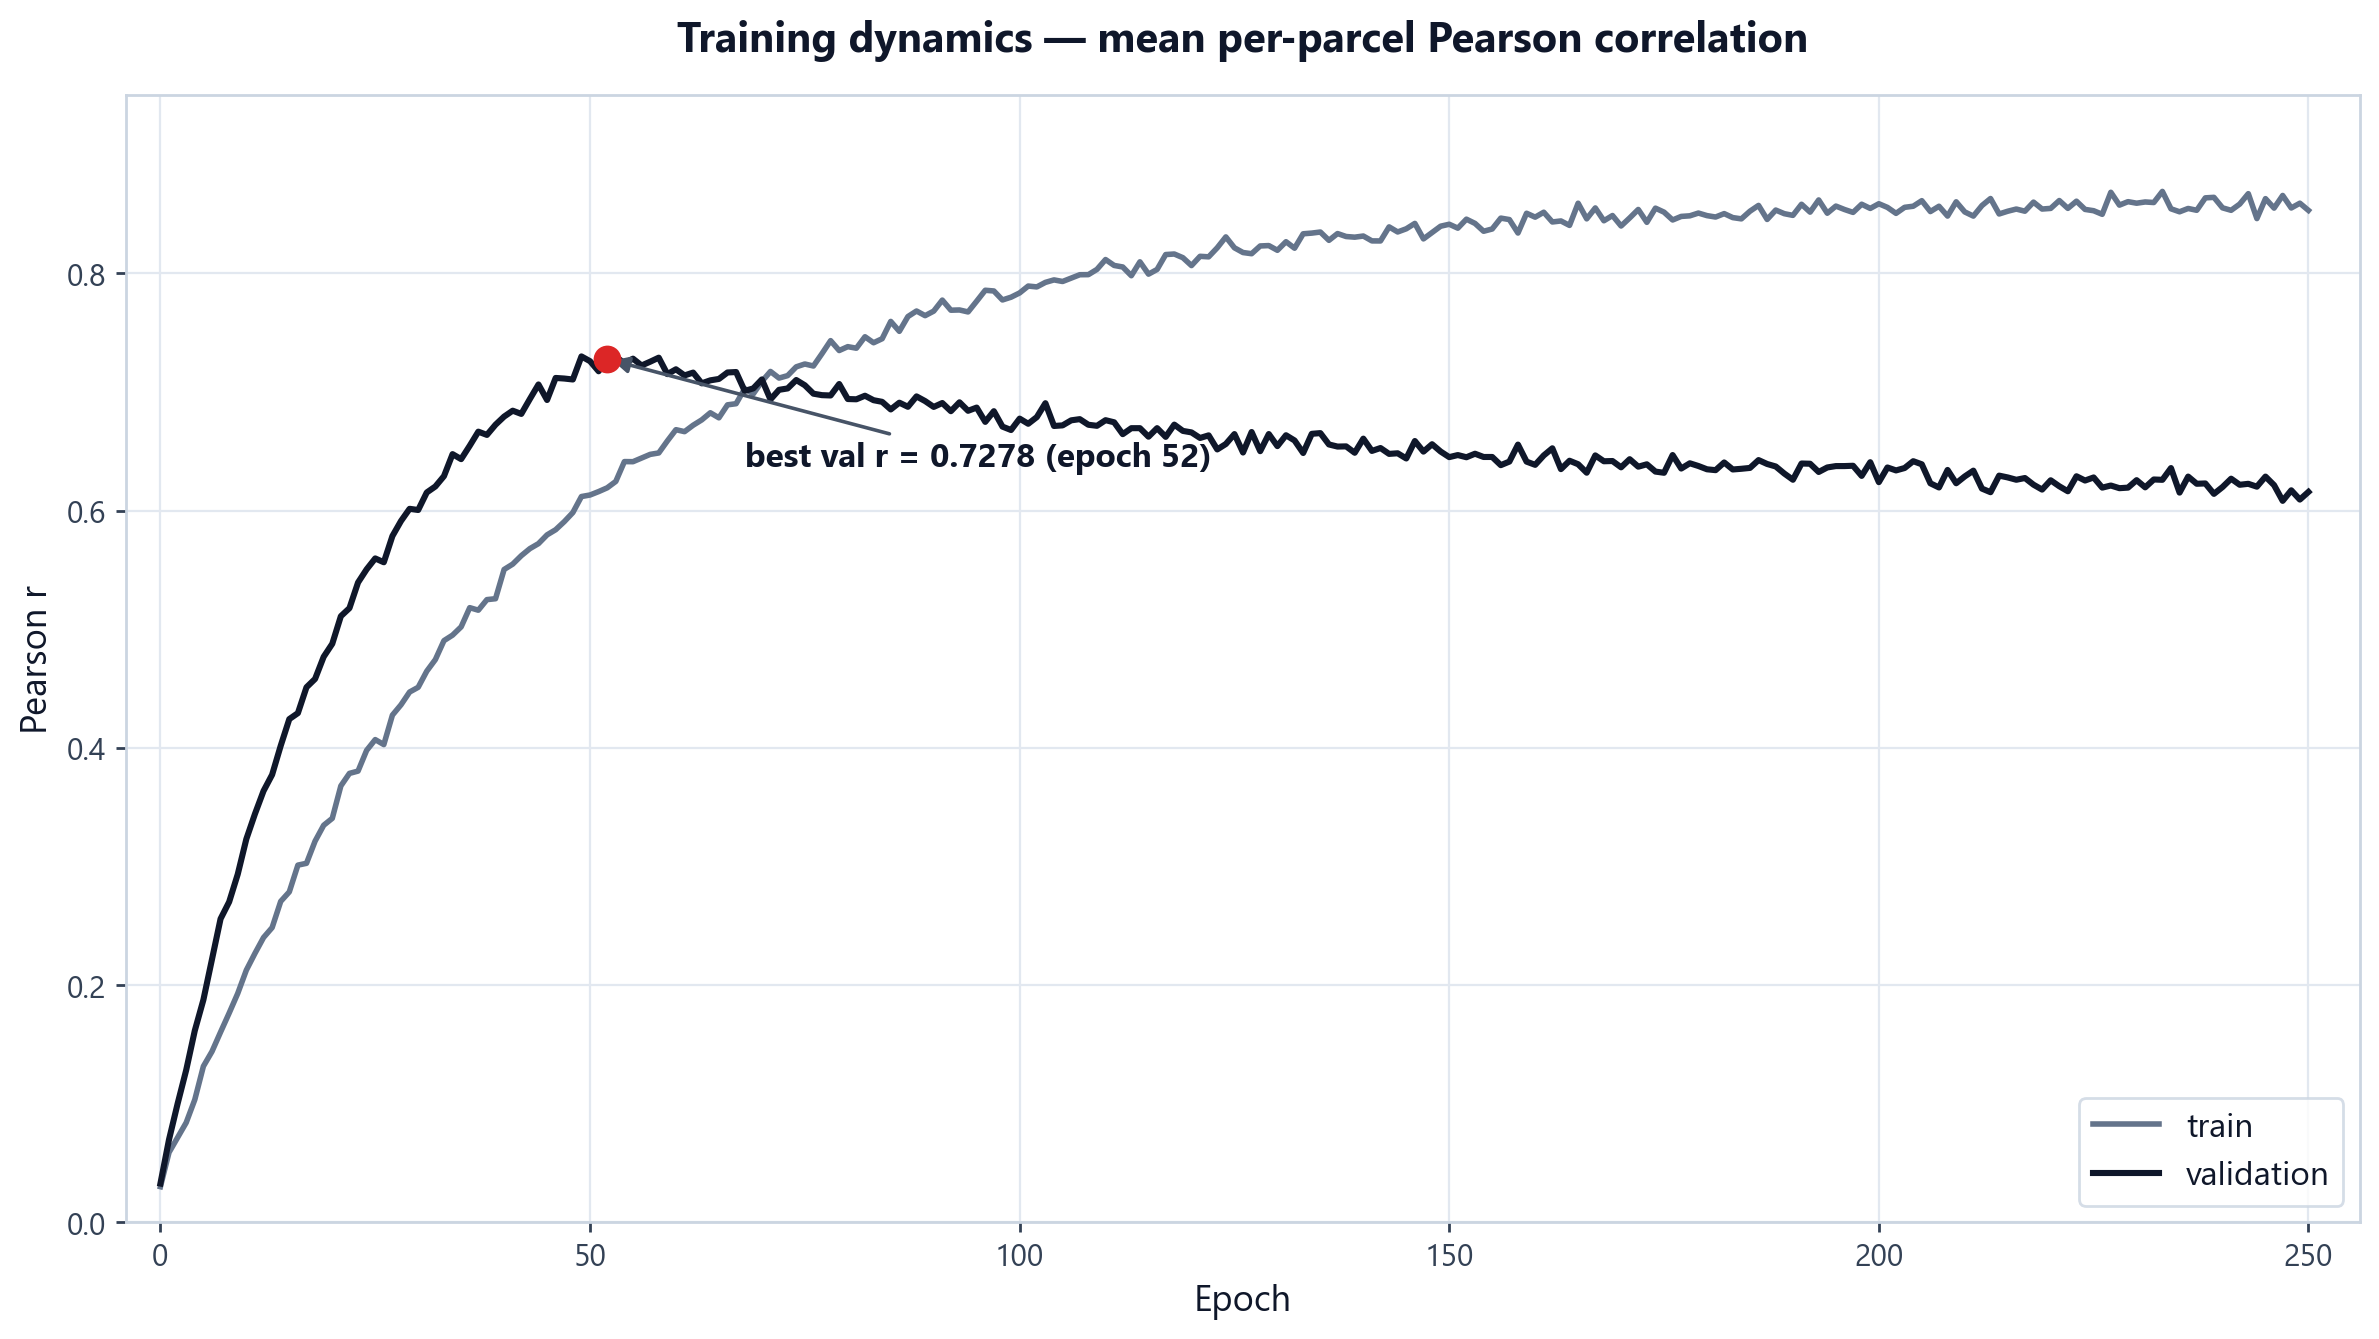
\includegraphics[width=0.95\textwidth]{assets/training_results.png}
\caption{Динамика обучения: средний попарцеллярный Pearson~$r$ на
обучении и валидации; лучшая точка $r = 0{,}7278$ (эпоха~$52$)
отмечена маркером (фигура проекта:
\texttt{assets/training\_results.png}).}
\label{fig:training}
\end{figure}

\begin{figure}[H]
\centering
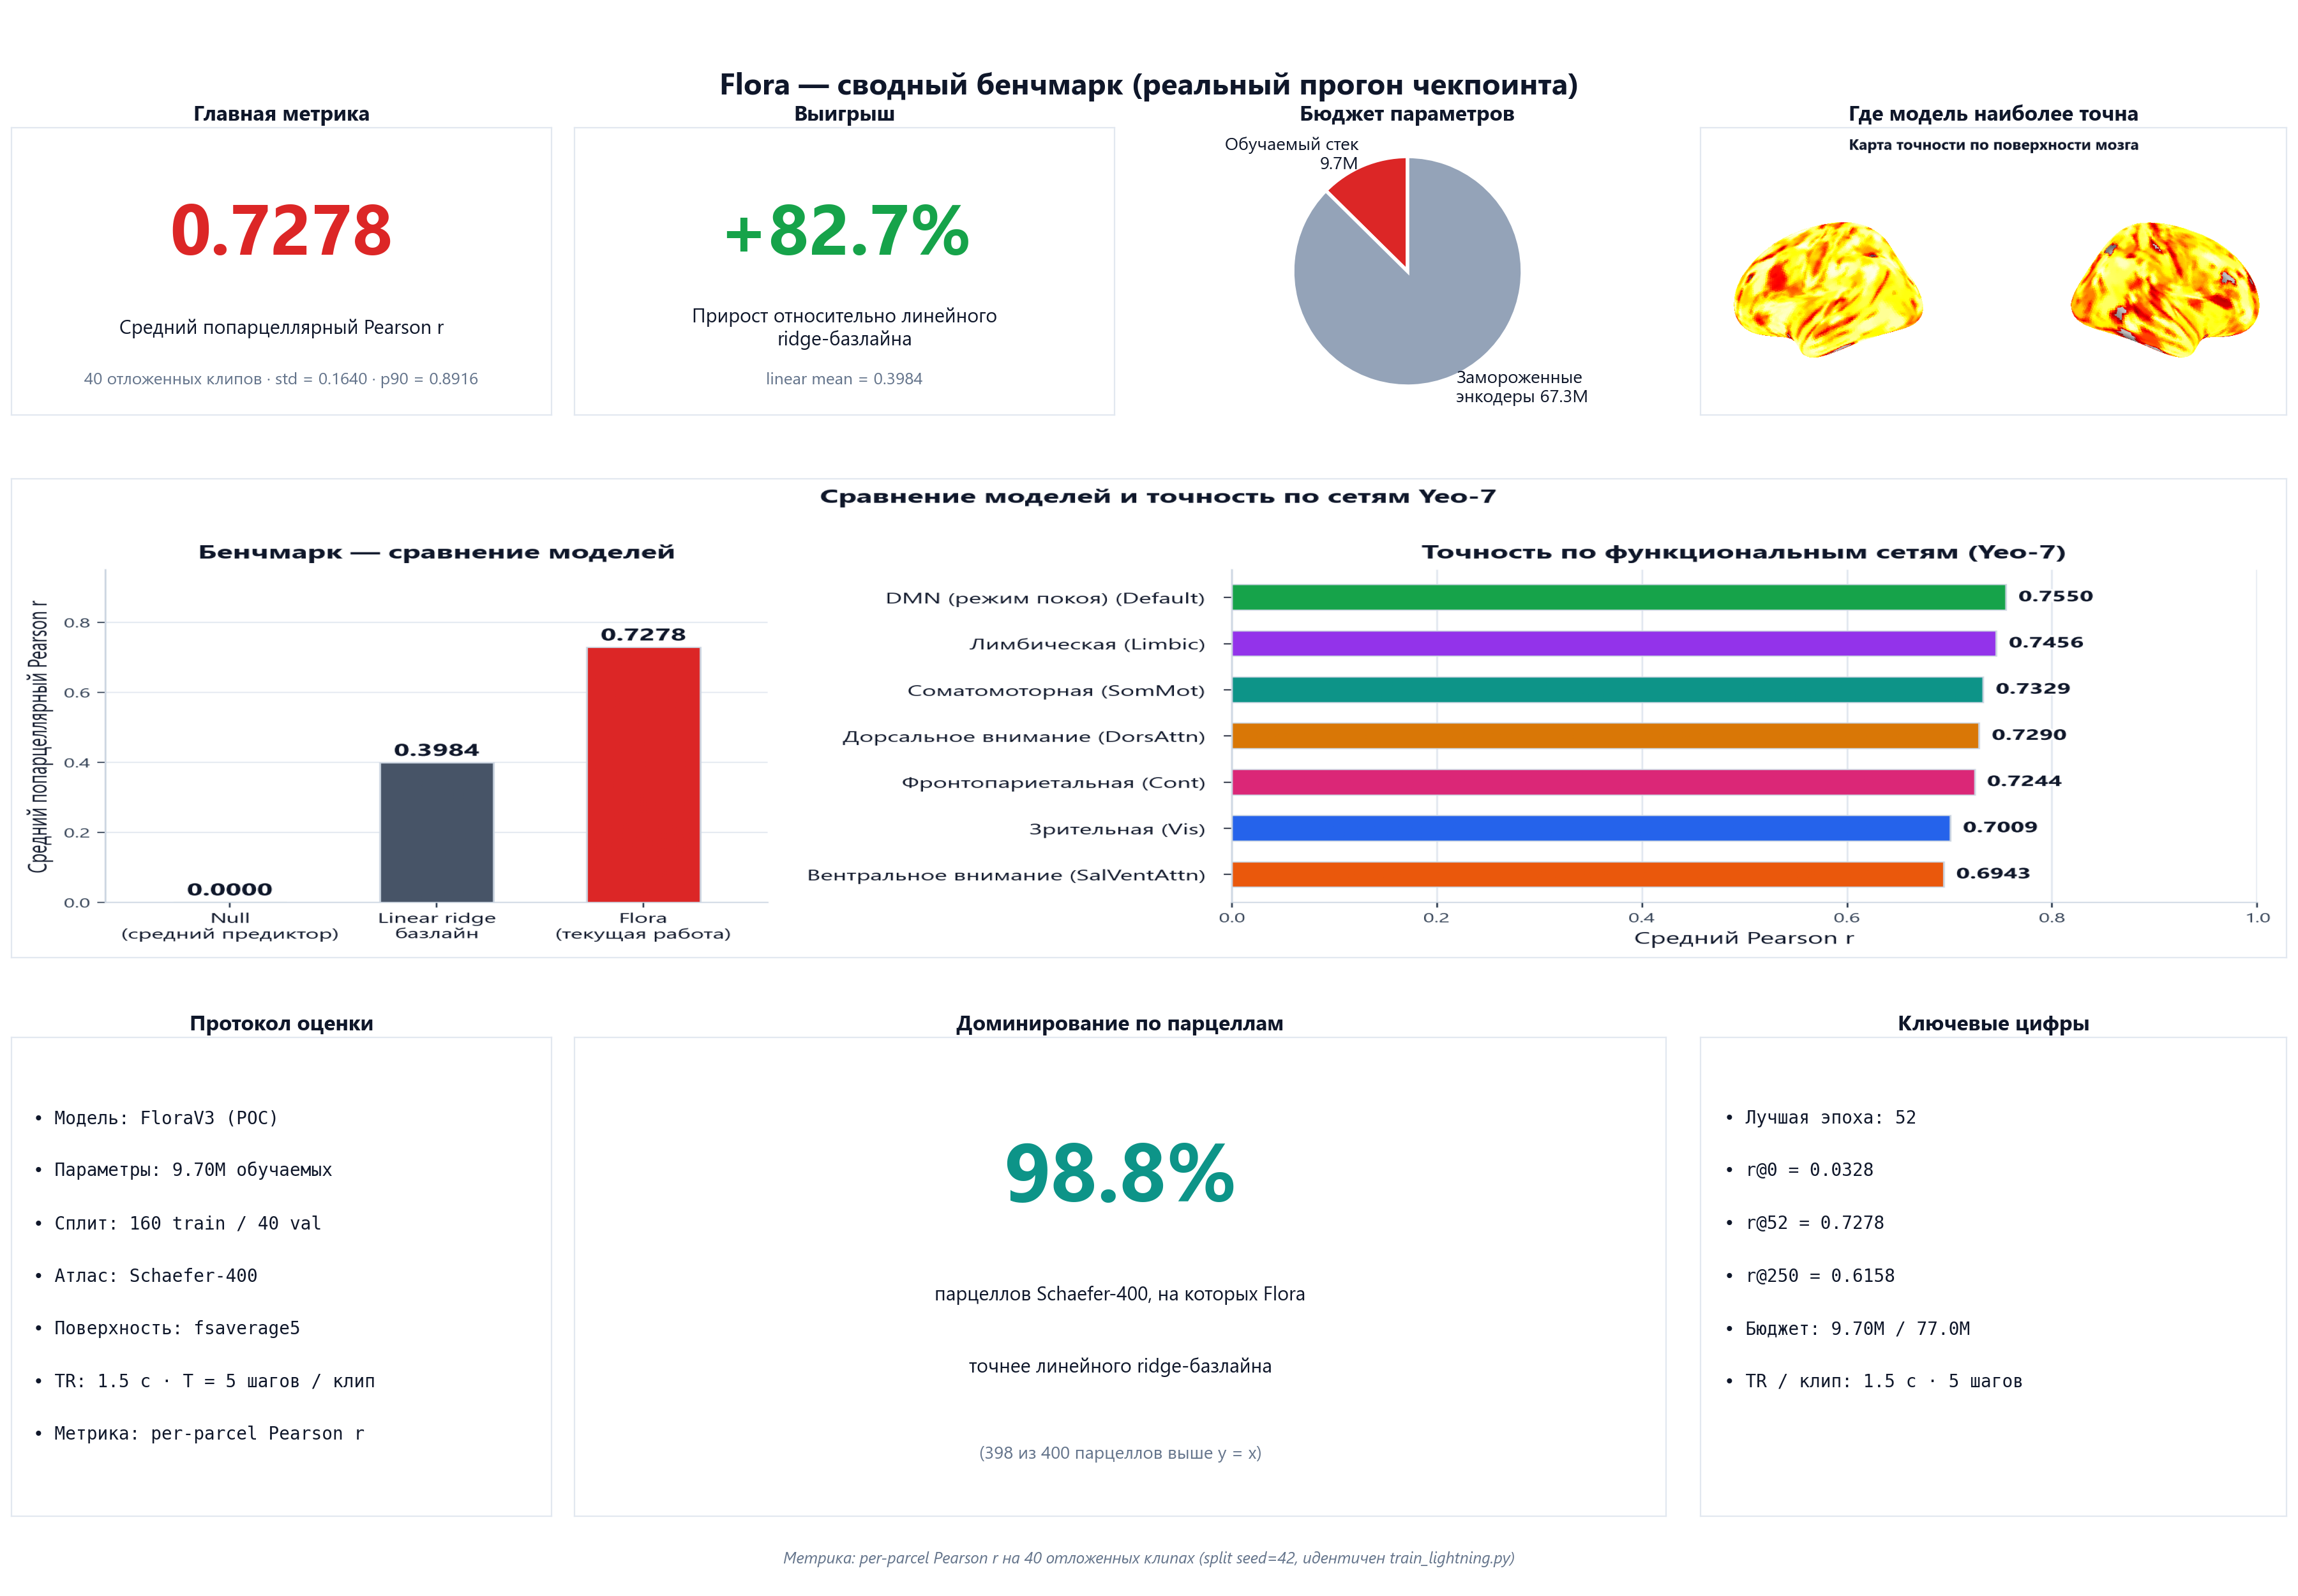
\includegraphics[width=0.98\textwidth]{benchmarks/figures/10_dashboard.png}
\caption{Сводная панель бенчмарка (реальный прогон чекпоинта):
итоговая метрика, выигрыш над линейным базлайном, бюджет параметров,
карточка протокола, сравнение моделей и точность по сетям Yeo-7
(\texttt{benchmarks/figures/10\_dashboard.png}).}
\label{fig:dashboard}
\end{figure}

\subsection{Сравнение с базовыми моделями}
\label{sec:benchmarks}

\begin{table}[H]
\centering
\caption{Бенчмарк на 40 отложенных клипах (per-parcel Pearson~$r$,
модель против эталона; фактический прогон). Линейный ridge-базлайн
обучен на тех же признаках и том же сплите.}
\label{tab:benchmark}
\small
\begin{tabular}{lcccccc}
\toprule
Модель & mean & std & p50 & p90 & max & Параметры \\
\midrule
Null (среднее по train) & 0{,}0000 & --- & --- & --- & --- & 0 \\
Linear ridge & 0{,}3984 & 0{,}1333 & 0{,}3983 & 0{,}5728 & 0{,}7460 & 0{,}56~млн \\
\textbf{Flora} & \textbf{0{,}7278} & 0{,}1640 & 0{,}7590 & 0{,}8916 & 0{,}9457 & 9{,}70~млн \\
\bottomrule
\end{tabular}
\end{table}

Flora превосходит линейный базлайн на $+82{,}7\%$ по средней метрике
и точнее него в \textbf{$98{,}8\%$} из $400$~парцеллов
(\cref{tab:benchmark,fig:scatter,fig:hist}). Pareto-вид
<<точность против бюджета параметров>> (\cref{fig:pareto})
показывает, что обучаемый стек из $9{,}7$~млн параметров занимает
эффективную точку фронта.

\begin{figure}[H]
\centering
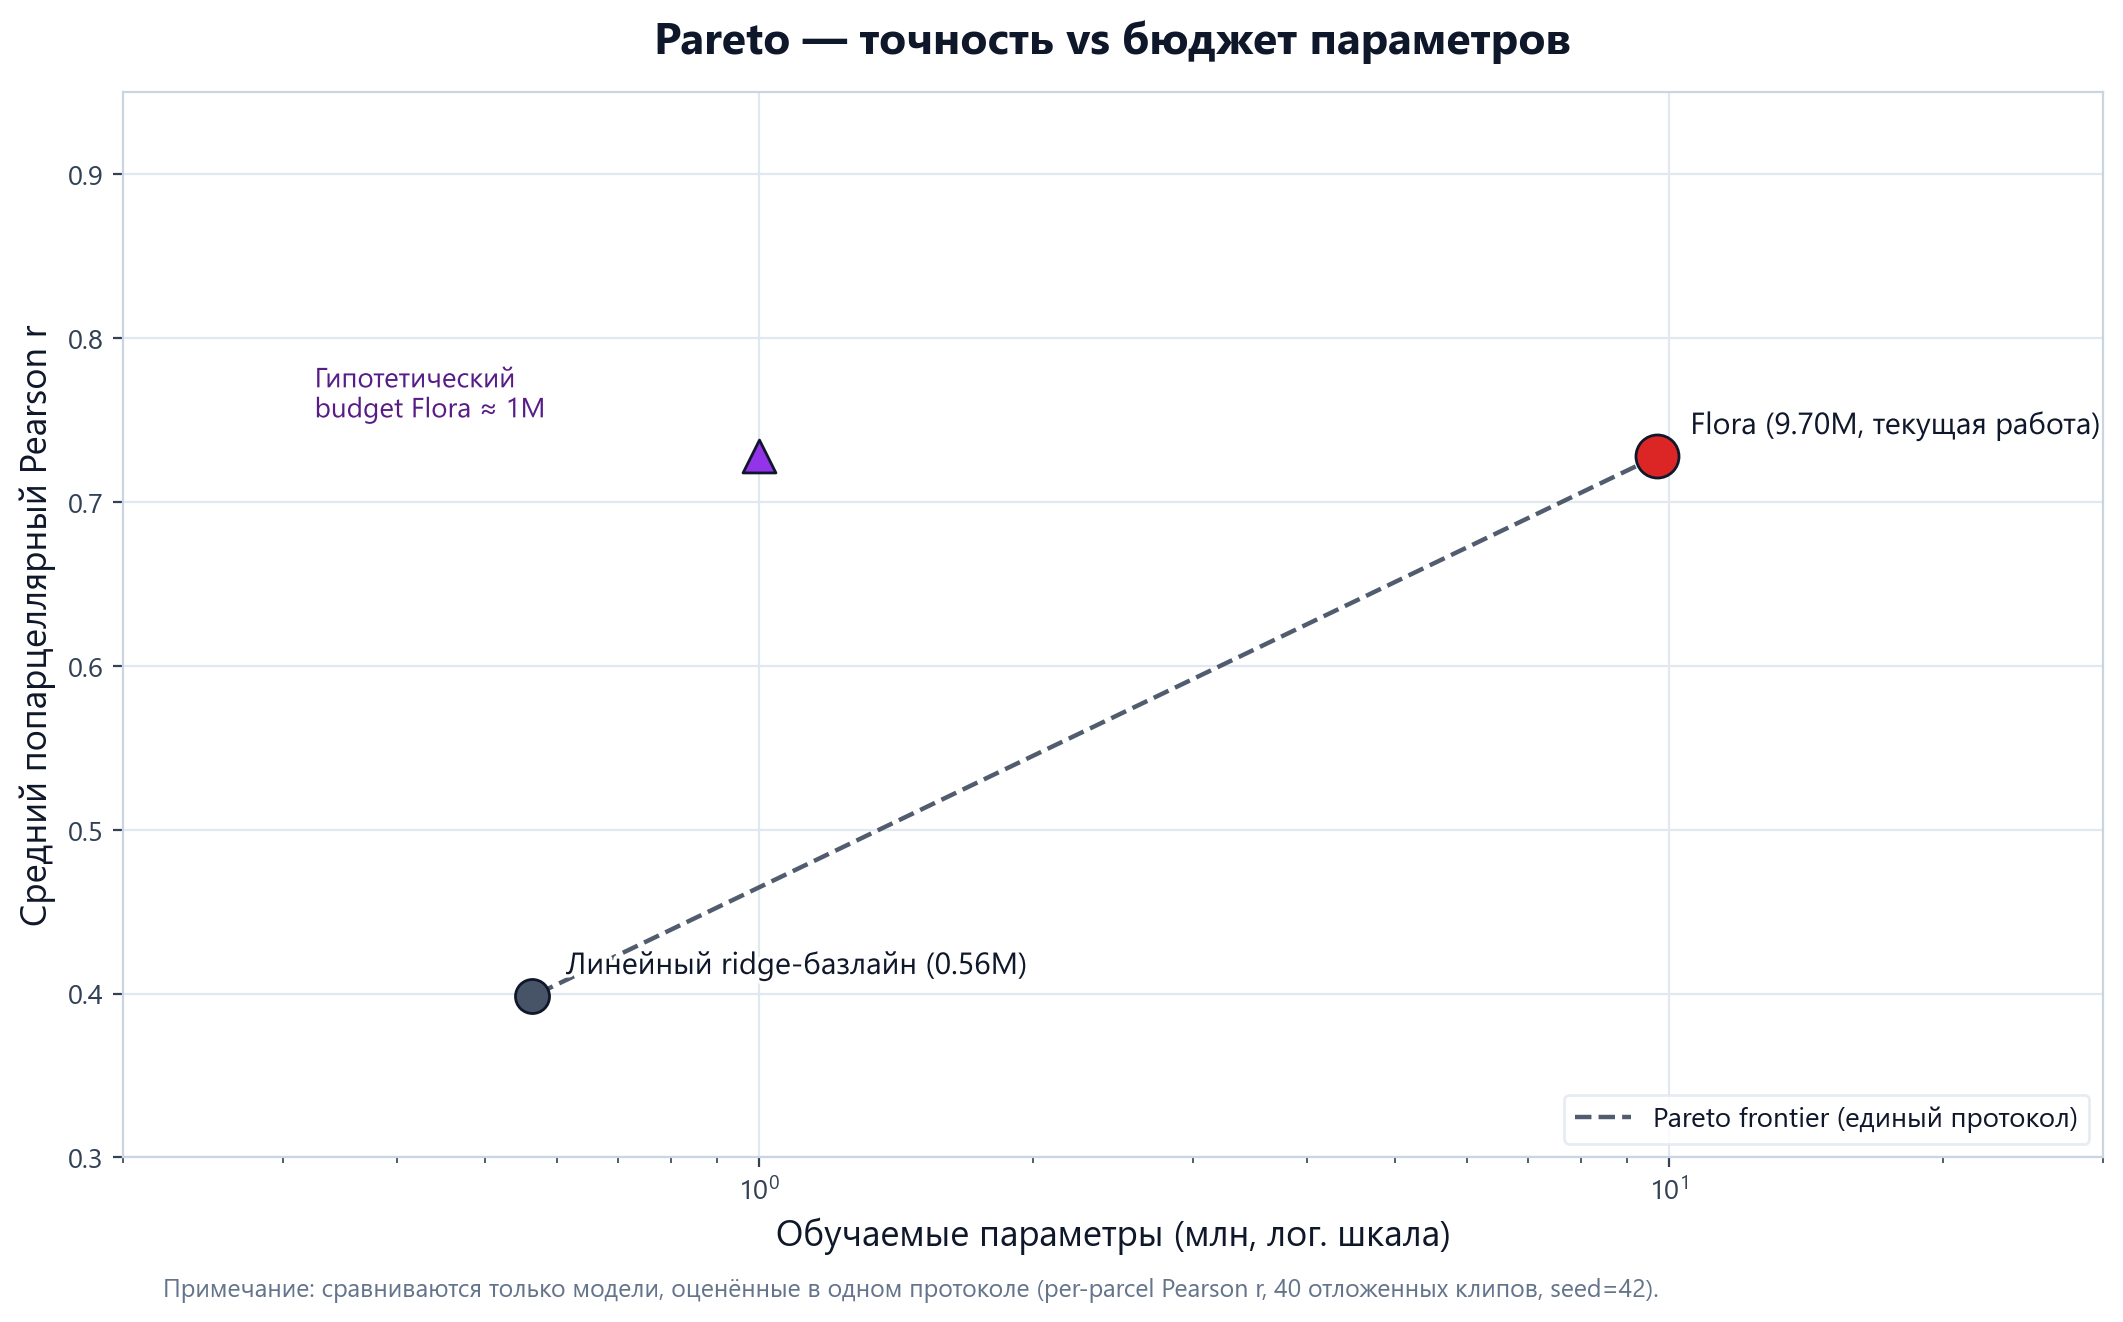
\includegraphics[width=0.9\textwidth]{benchmarks/figures/01_pareto_frontier.png}
\caption{Pareto-график <<точность -- бюджет параметров>>
(лог-шкала). Flora и линейный базлайн измерены в едином протоколе
проекта (\texttt{benchmarks/figures/01\_pareto\_frontier.png}).}
\label{fig:pareto}
\end{figure}

\begin{figure}[H]
\centering
\begin{subfigure}[b]{0.49\textwidth}
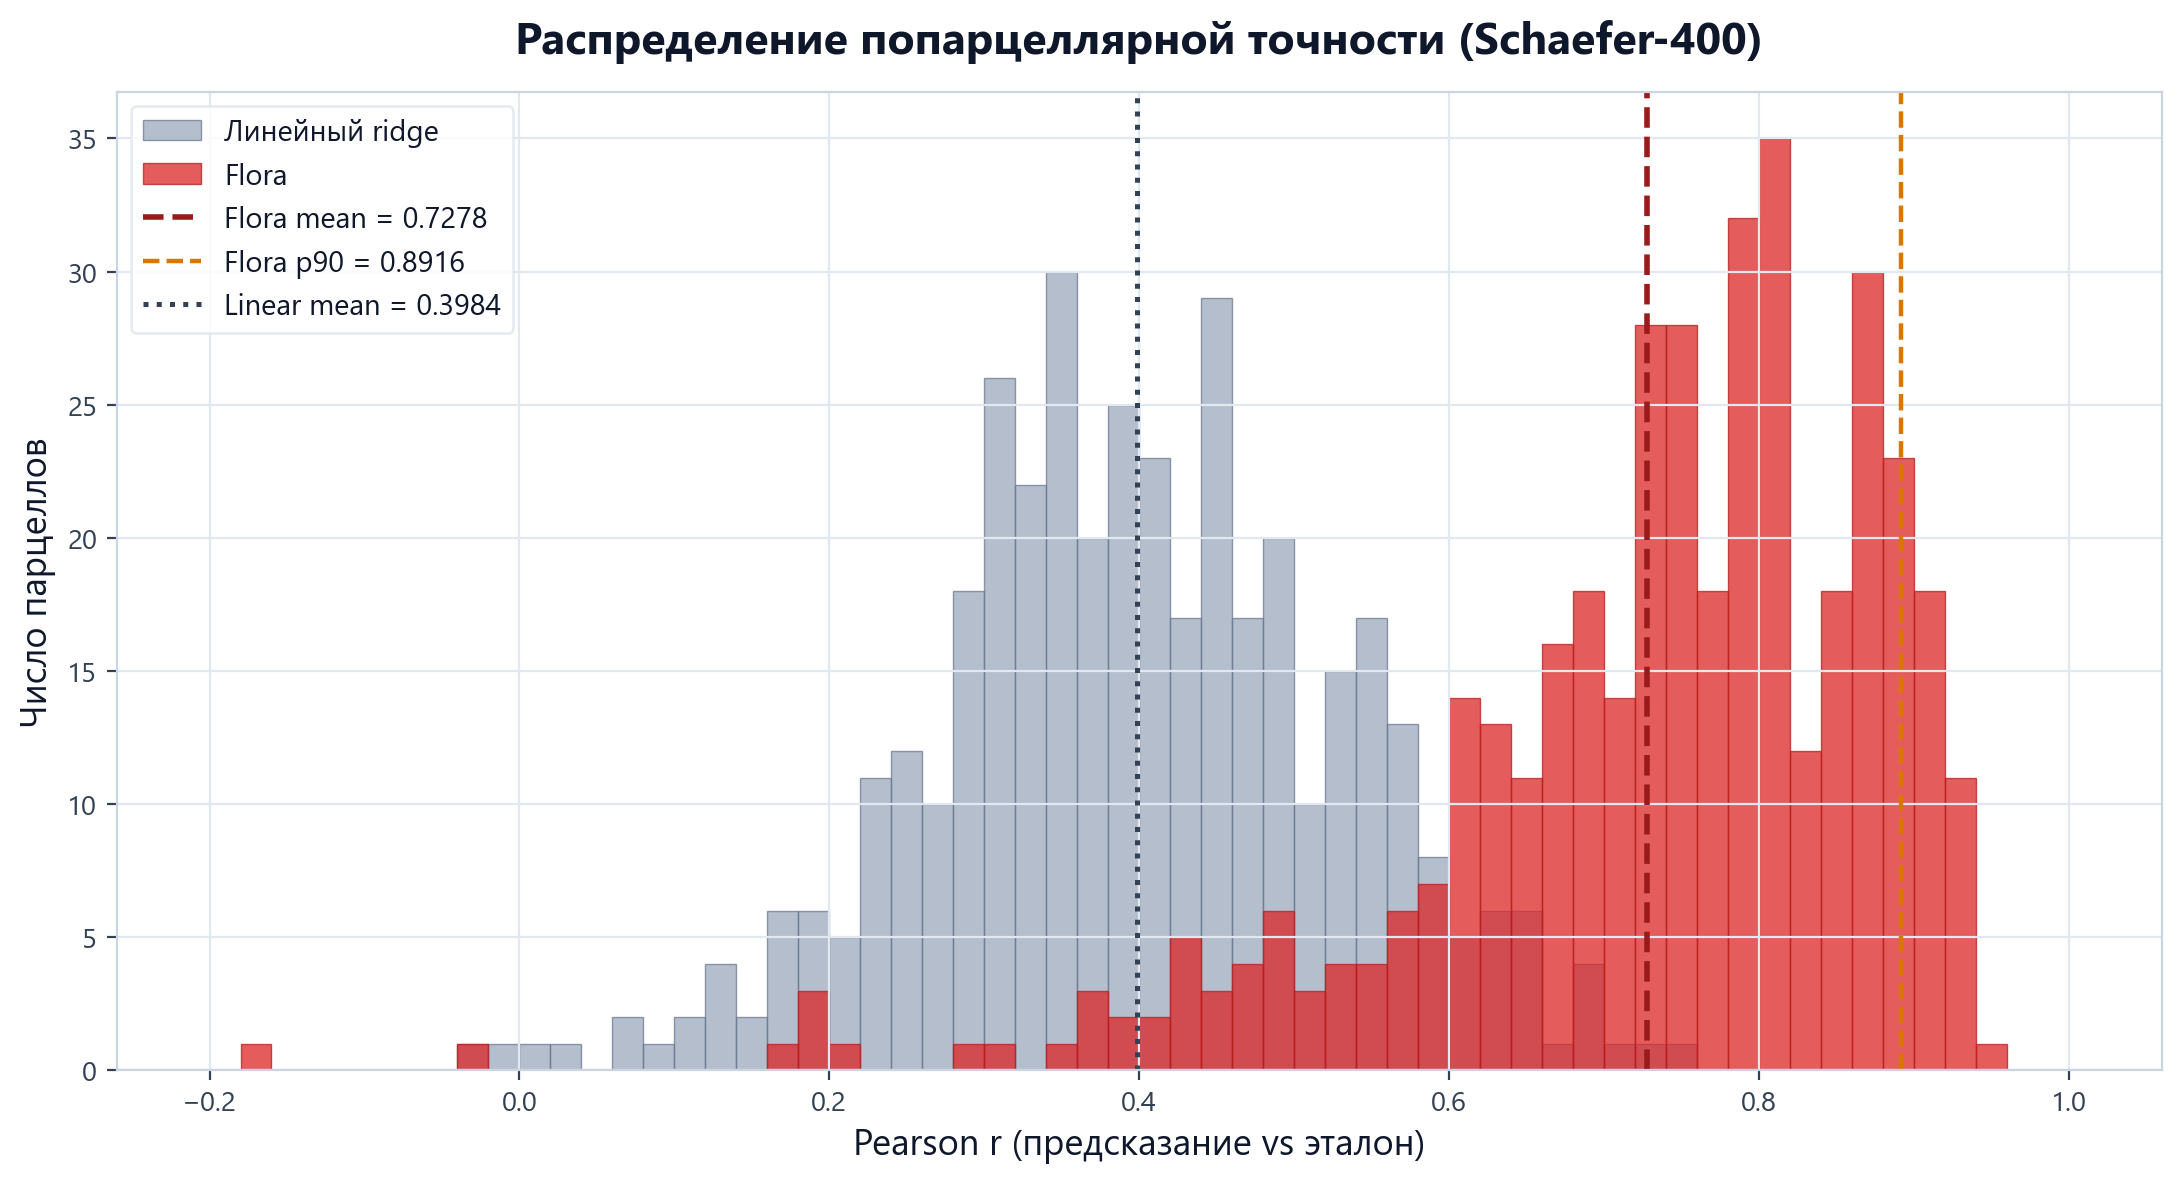
\includegraphics[width=\textwidth]{benchmarks/figures/03_parcel_histogram.png}
\caption{Распределение попарцеллярной точности.}
\label{fig:hist}
\end{subfigure}\hfill
\begin{subfigure}[b]{0.49\textwidth}
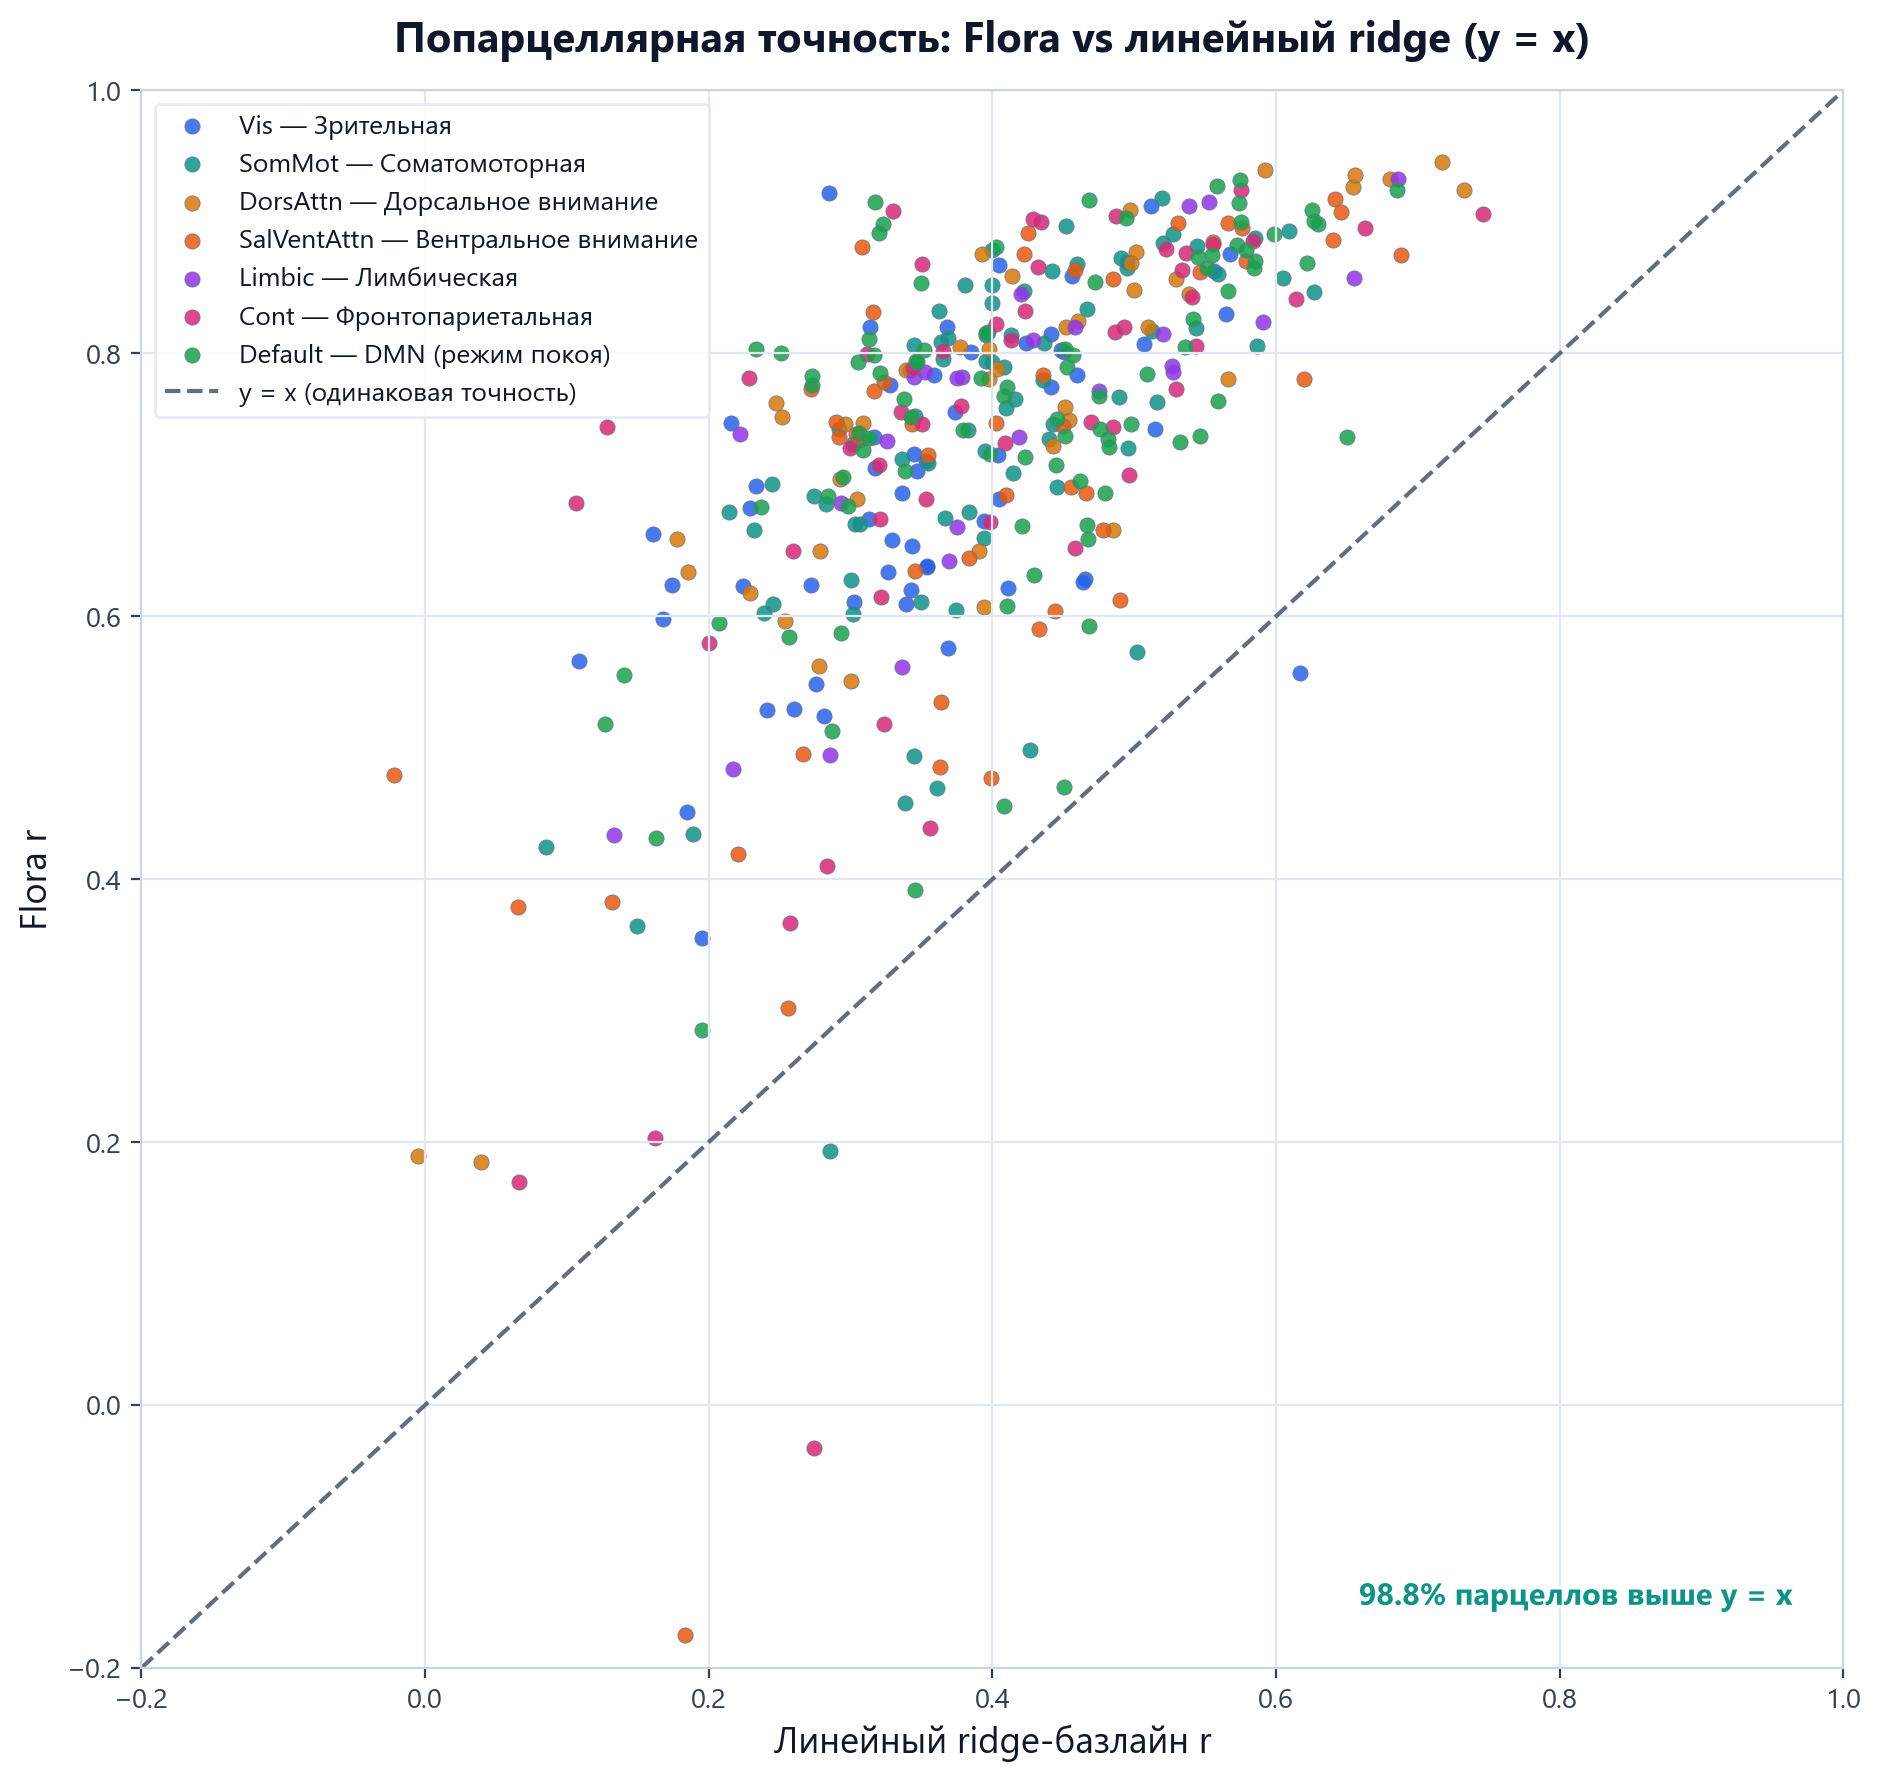
\includegraphics[width=\textwidth]{benchmarks/figures/08_flora_vs_linear_scatter.png}
\caption{Flora против линейного базлайна по парцеллам.}
\label{fig:scatter}
\end{subfigure}
\caption{Попарцеллярный анализ точности: (a) гистограммы $400$
значений $r$ для Flora и линейного базлайна; (b) scatter с
линией $y = x$: $98{,}8\%$ парцеллов выше диагонали
(\texttt{benchmarks/figures/03\_parcel\_histogram.png},
\texttt{benchmarks/figures/08\_flora\_vs\_linear\_scatter.png}).}
\label{fig:per-parcel}
\end{figure}

\subsection{Пространственное распределение точности}
\label{sec:zones}

Попарцеллярная точность была спроецирована на атлас Schaefer-400 и
поверхность fsaverage5 (\cref{fig:zones,fig:glass}). Наиболее точно
модель предсказывает парцеллы дорсального внимания и DMN:
топ-3 зоны~--- DorsAttn$\cdot$LH$\cdot$Post~\#14 ($r = 0{,}946$),
DorsAttn$\cdot$LH$\cdot$FEF~\#4 ($0{,}939$),
DorsAttn$\cdot$LH$\cdot$FEF~\#1 ($0{,}936$); полный топ-15~--- на
\cref{fig:top15}. Разбиение по сетям Yeo-7
(\cref{tab:networks,fig:netpareto,fig:radar}): лучше всего
предсказываются DMN ($0{,}7550$) и лимбическая сеть ($0{,}7456$),
хуже всего~--- вентральное внимание ($0{,}6943$) и зрительная
сеть ($0{,}7009$), что согласуется с тем, что ранняя зрительная
кора обслуживается покадровым видео-энкодером без явной временной
динамики.

\begin{table}[H]
\centering
\caption{Средняя точность по функциональным сетям Yeo-7
(фактический прогон).}
\label{tab:networks}
\small
\begin{tabular}{lccc}
\toprule
Сеть & Парцелл & Flora $r$ & Linear $r$ \\
\midrule
Default (DMN)              & 91 & 0{,}7550 & 0{,}4221 \\
Limbic                     & 26 & 0{,}7456 & 0{,}4156 \\
SomMot                     & 77 & 0{,}7329 & 0{,}3974 \\
DorsAttn                   & 46 & 0{,}7290 & 0{,}4006 \\
Cont (фронтопариетальная)  & 52 & 0{,}7244 & 0{,}3977 \\
Vis                        & 61 & 0{,}7009 & 0{,}3568 \\
SalVentAttn                & 47 & 0{,}6943 & 0{,}3972 \\
\bottomrule
\end{tabular}
\end{table}

\begin{figure}[H]
\centering
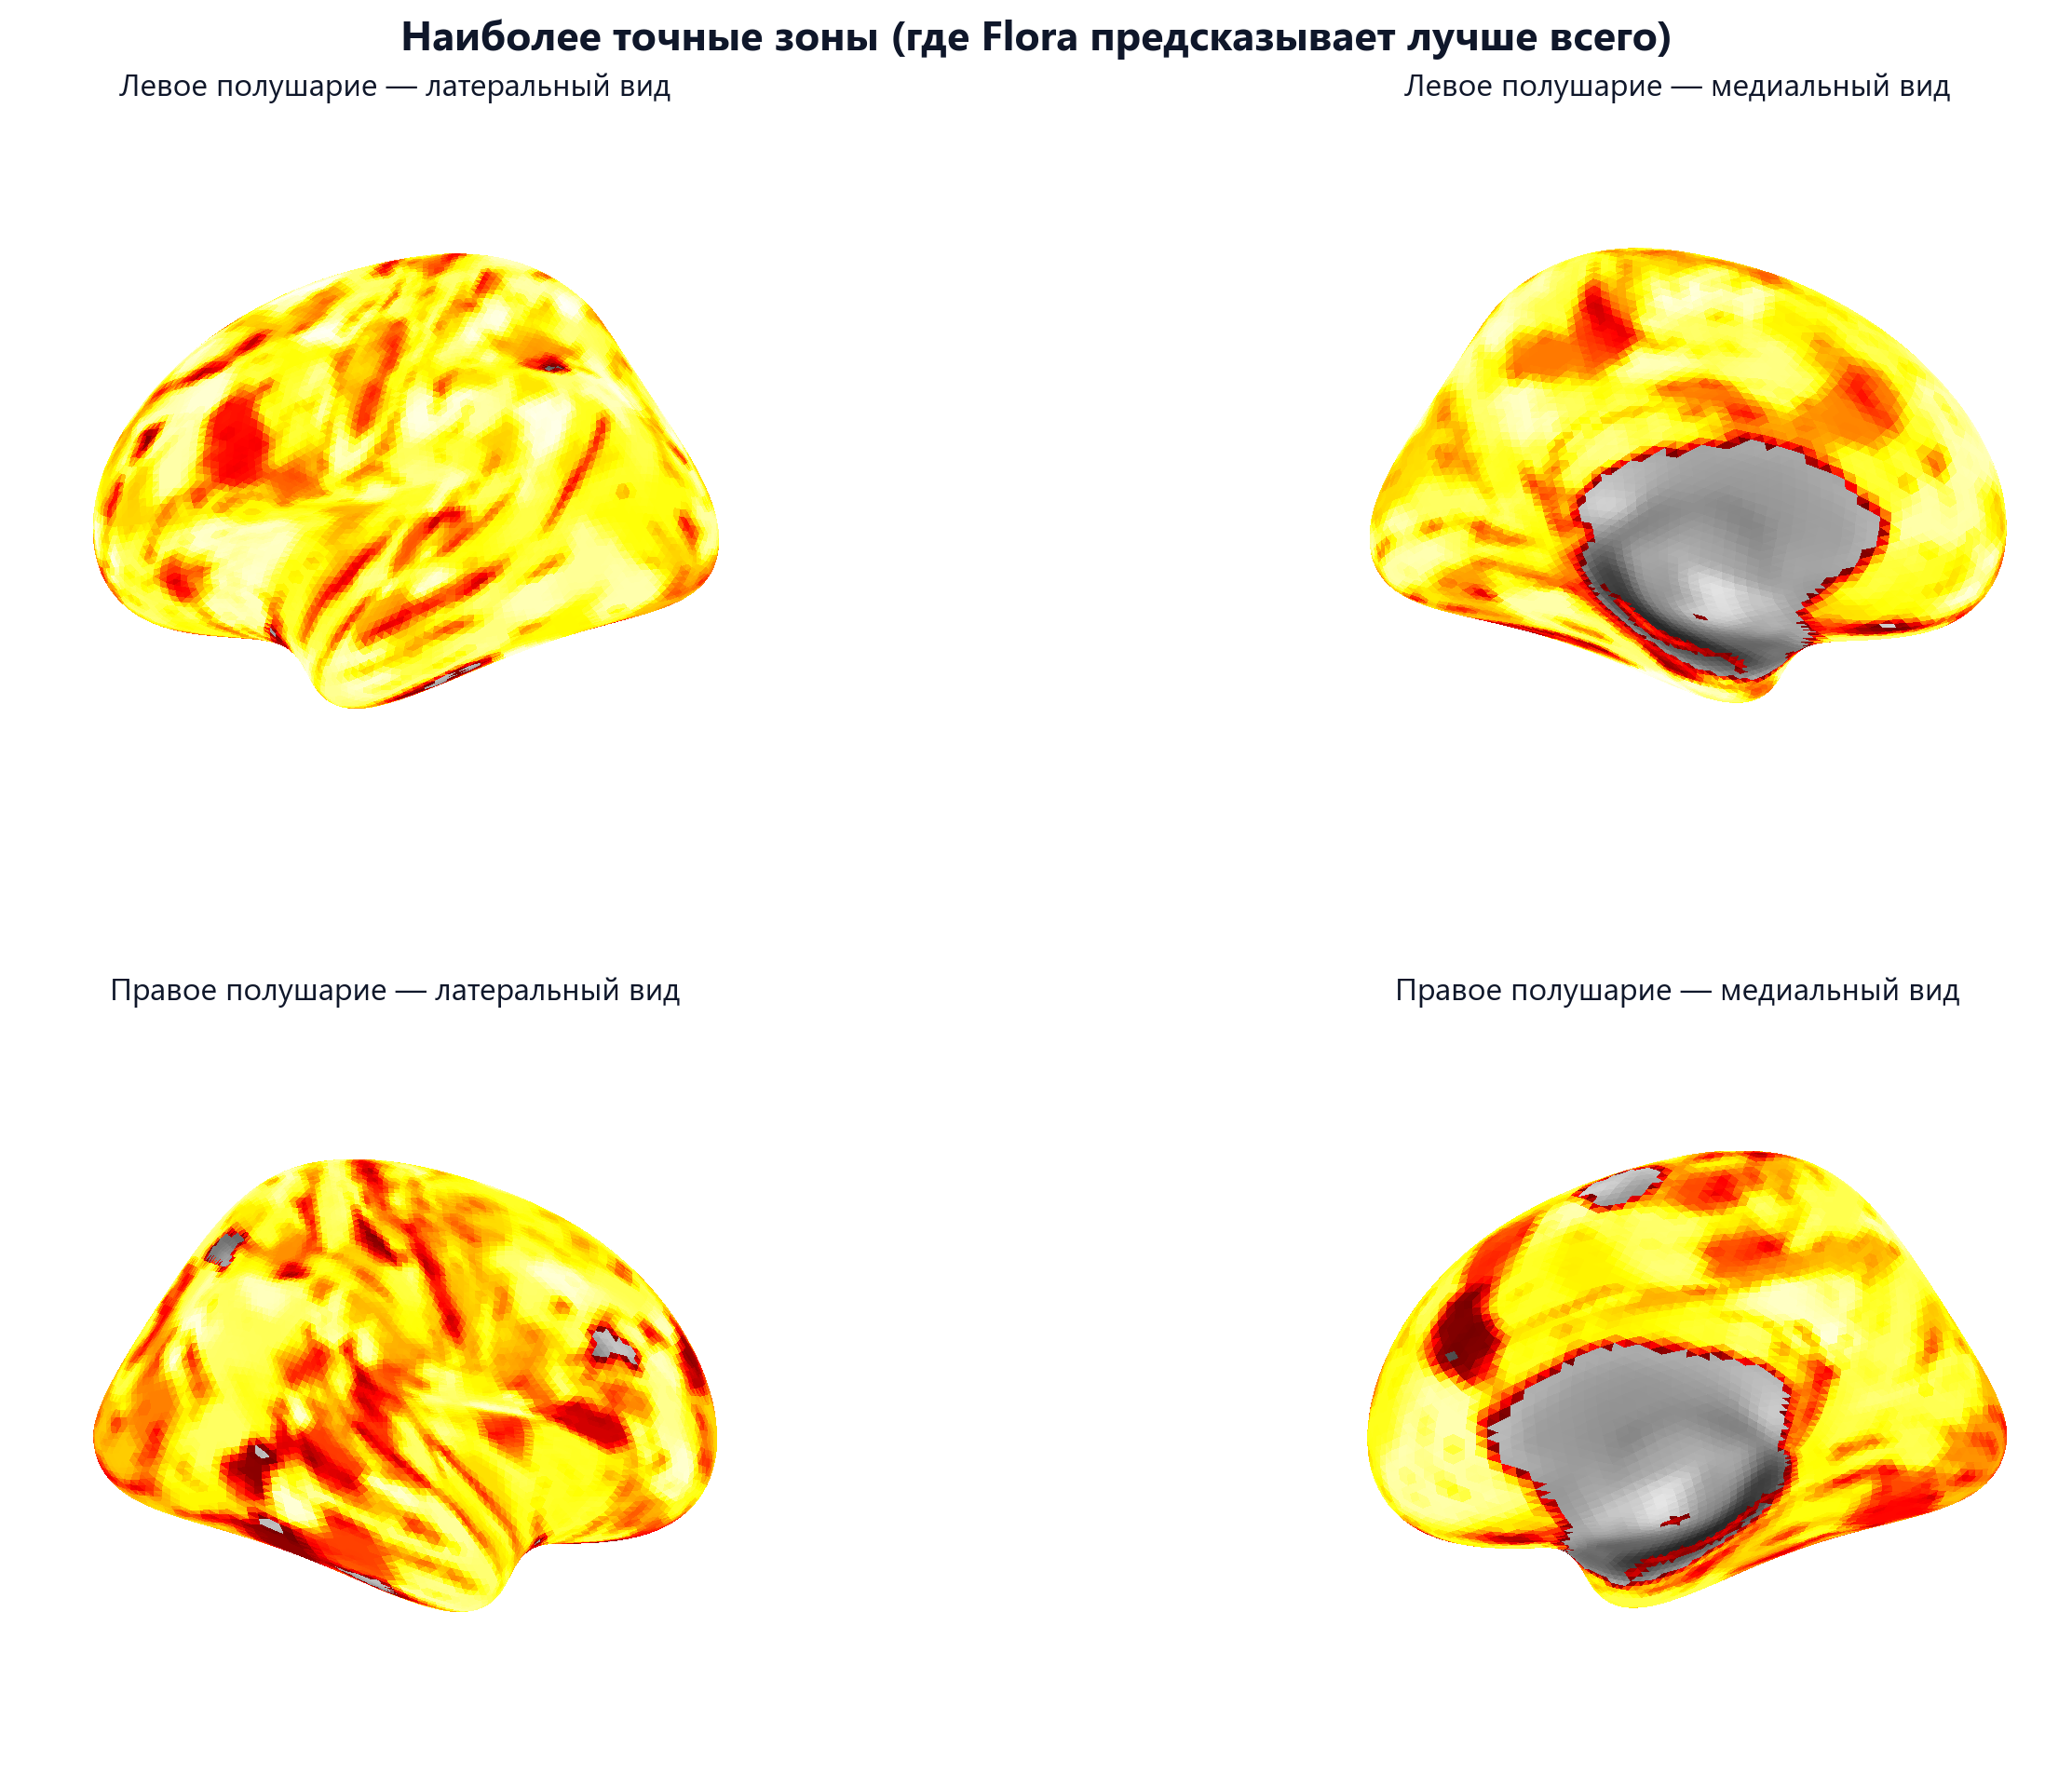
\includegraphics[width=0.95\textwidth]{benchmarks/figures/04_most_accurate_zones.png}
\caption{Most accurate zones: попарцеллярная точность Flora на
поверхности fsaverage5 (латеральный и медиальный виды обоих
полушарий, шкала $0$--$0{,}95$, палитра \emph{hot}). Видны зоны
максимальной точности в теменной коре и префронтальной коре
(\texttt{benchmarks/figures/04\_most\_accurate\_zones.png}).}
\label{fig:zones}
\end{figure}

\begin{figure}[H]
\centering
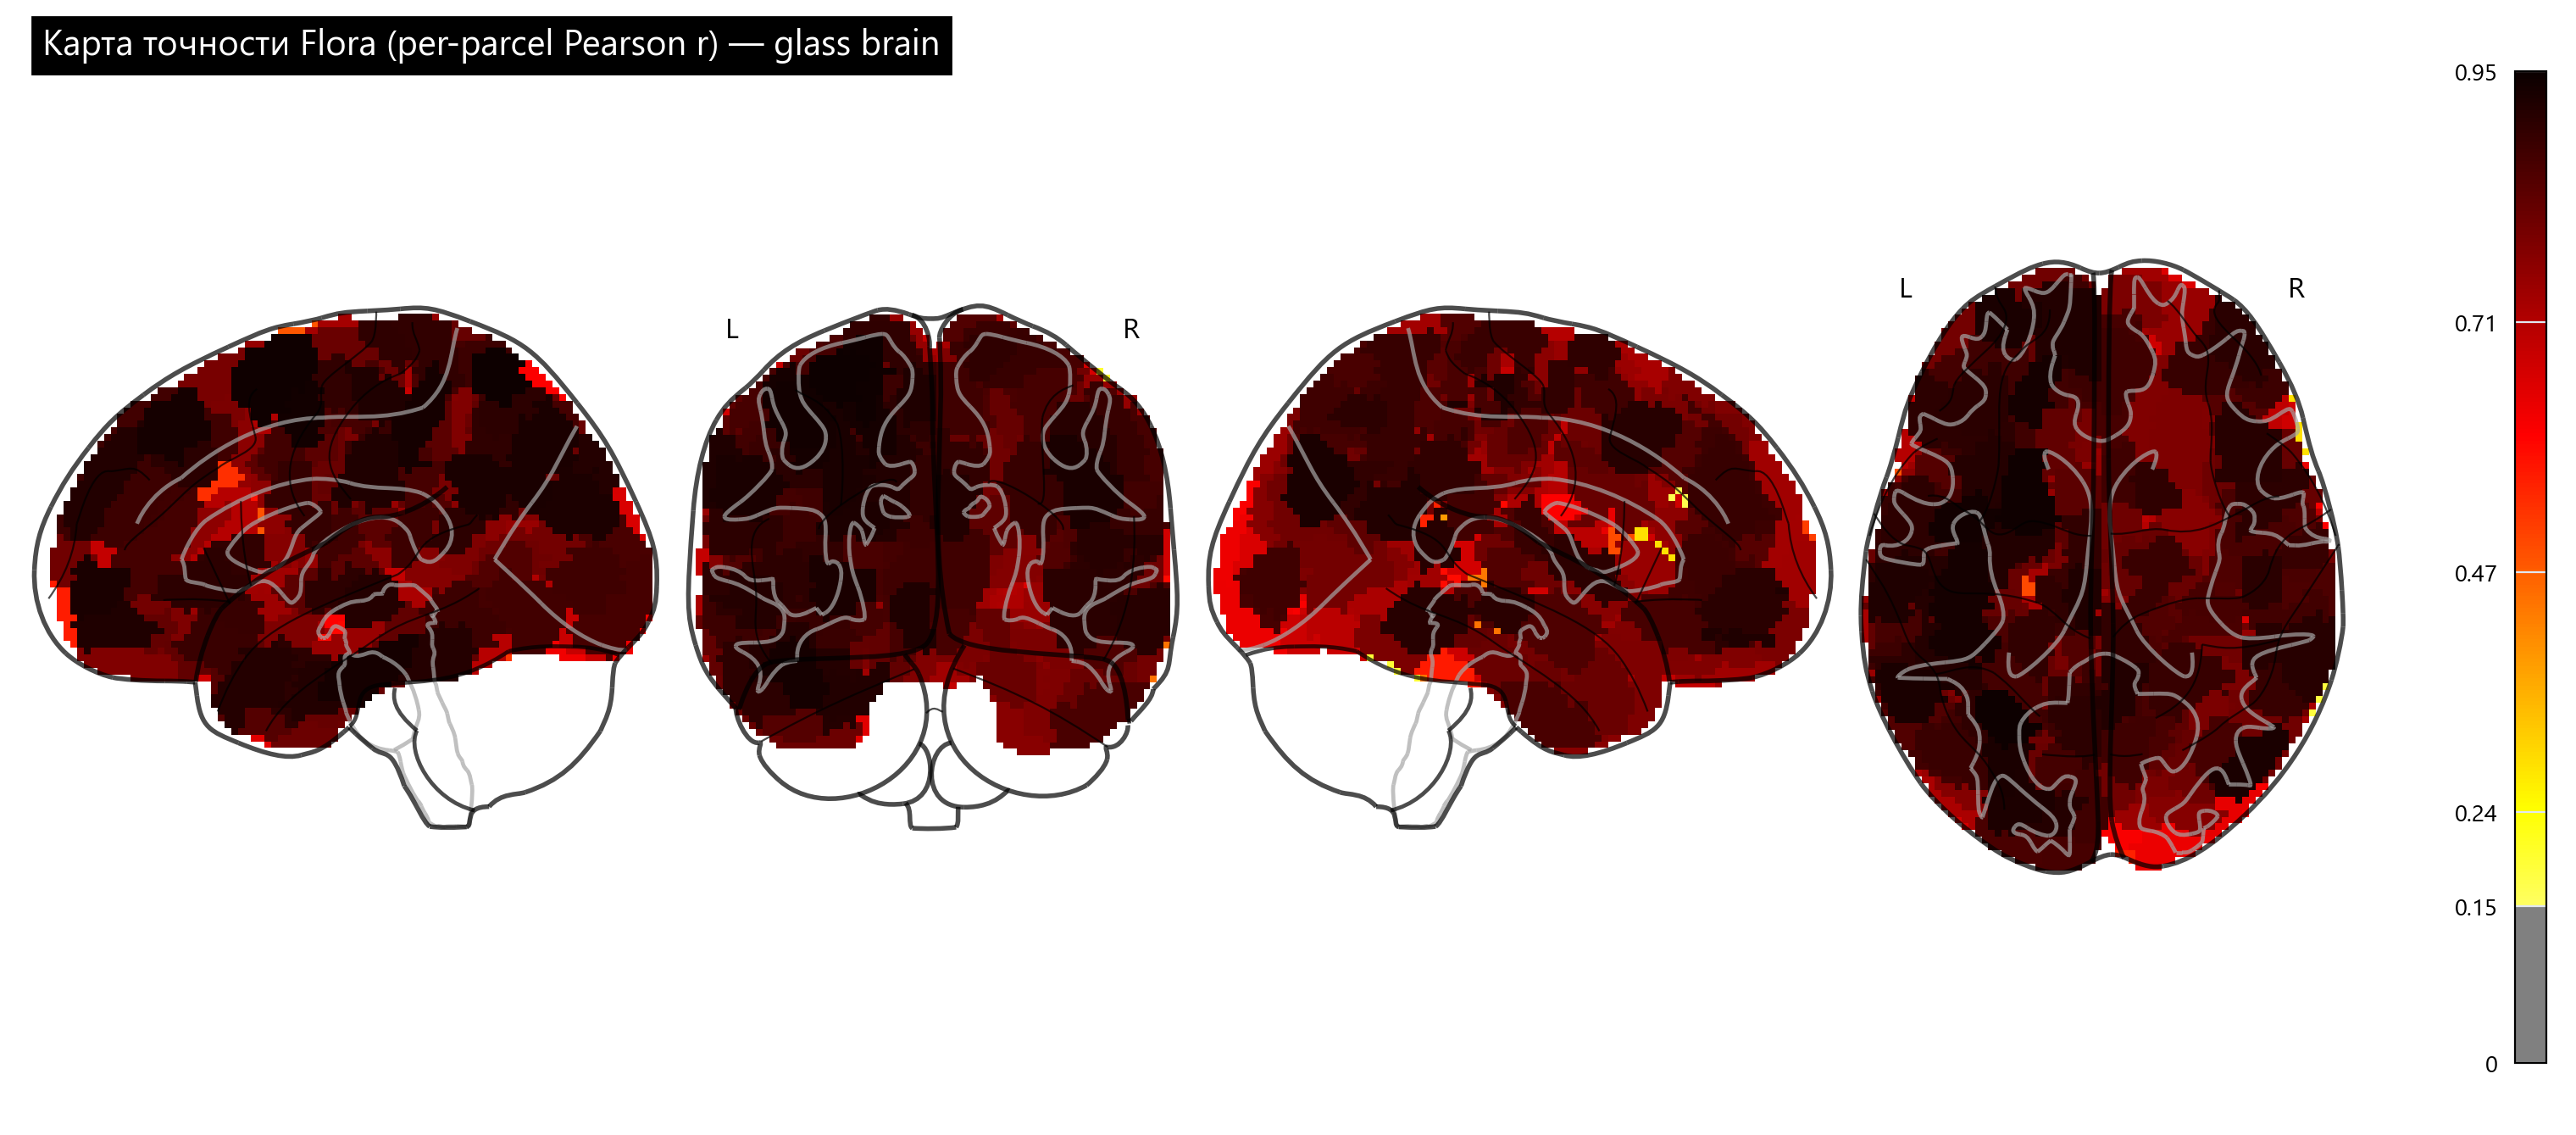
\includegraphics[width=0.95\textwidth]{benchmarks/figures/05_accuracy_glass_brain.png}
\caption{Glass-brain проекция карты точности (четыре среза:
сагиттальный, корональный, аксиальный)
(\texttt{benchmarks/figures/05\_accuracy\_glass\_brain.png}).}
\label{fig:glass}
\end{figure}

\begin{figure}[H]
\centering
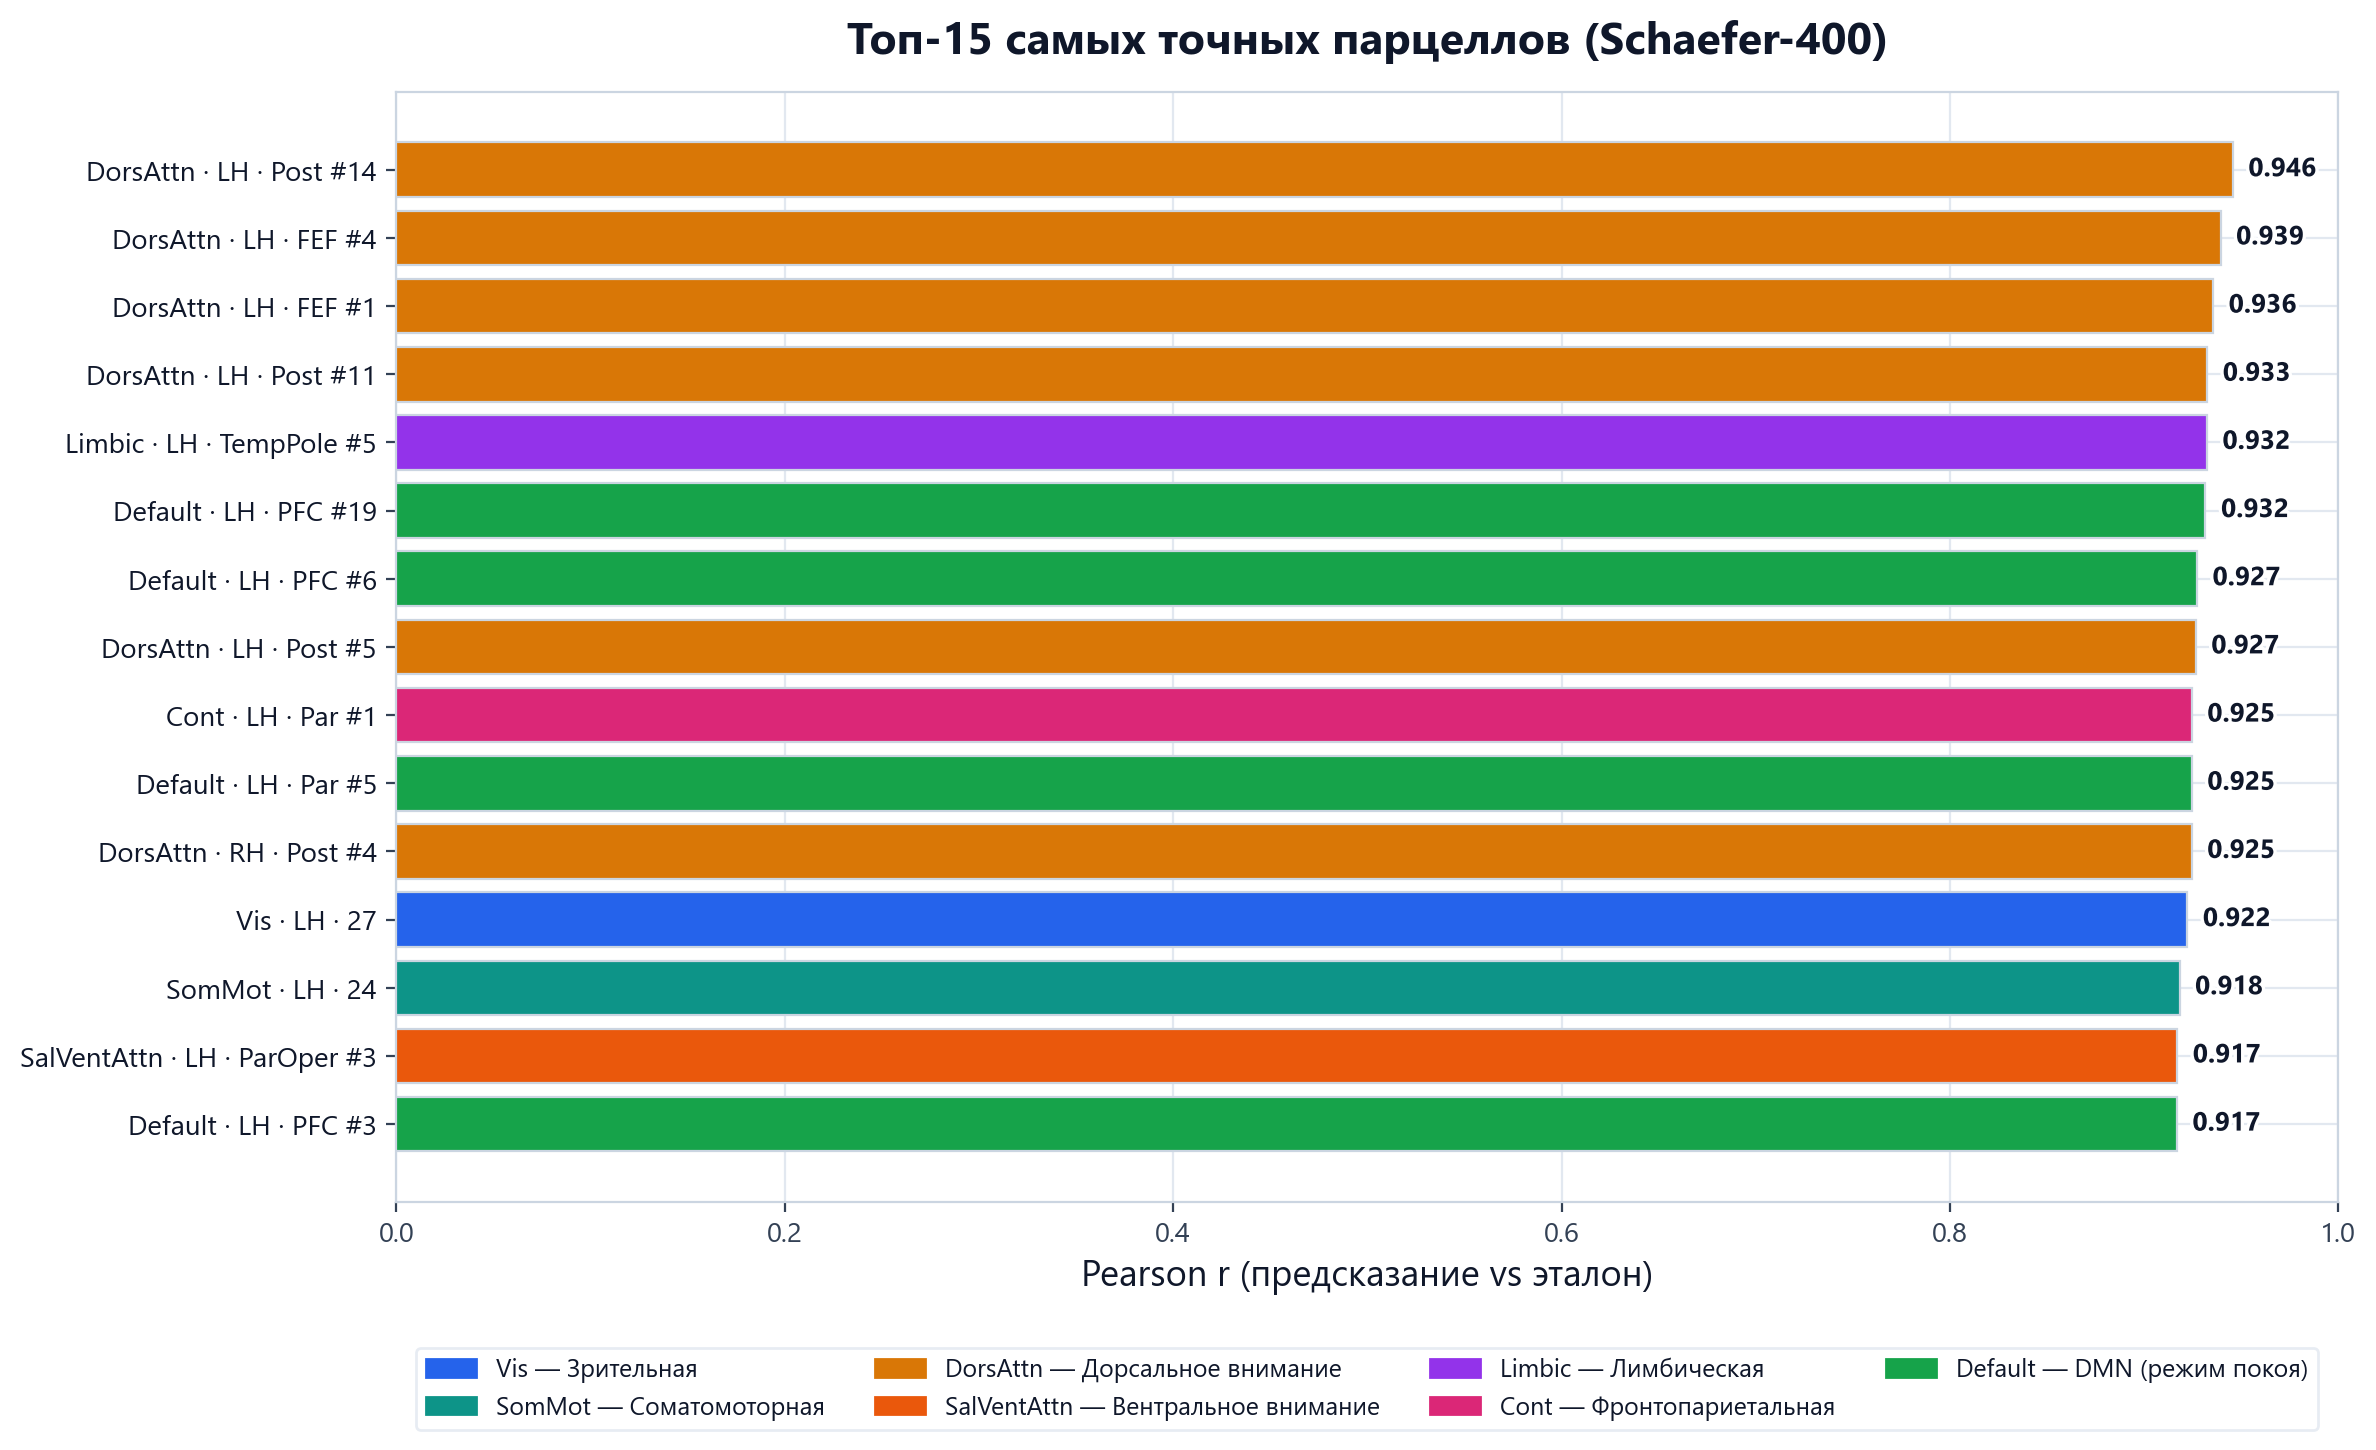
\includegraphics[width=0.9\textwidth]{benchmarks/figures/06_top15_zones.png}
\caption{Топ-15 наиболее точно предсказываемых парцеллов
Schaefer-400 с именами ROI и значениями $r$
(\texttt{benchmarks/figures/06\_top15\_zones.png}).}
\label{fig:top15}
\end{figure}

\begin{figure}[H]
\centering
\begin{subfigure}[b]{0.56\textwidth}
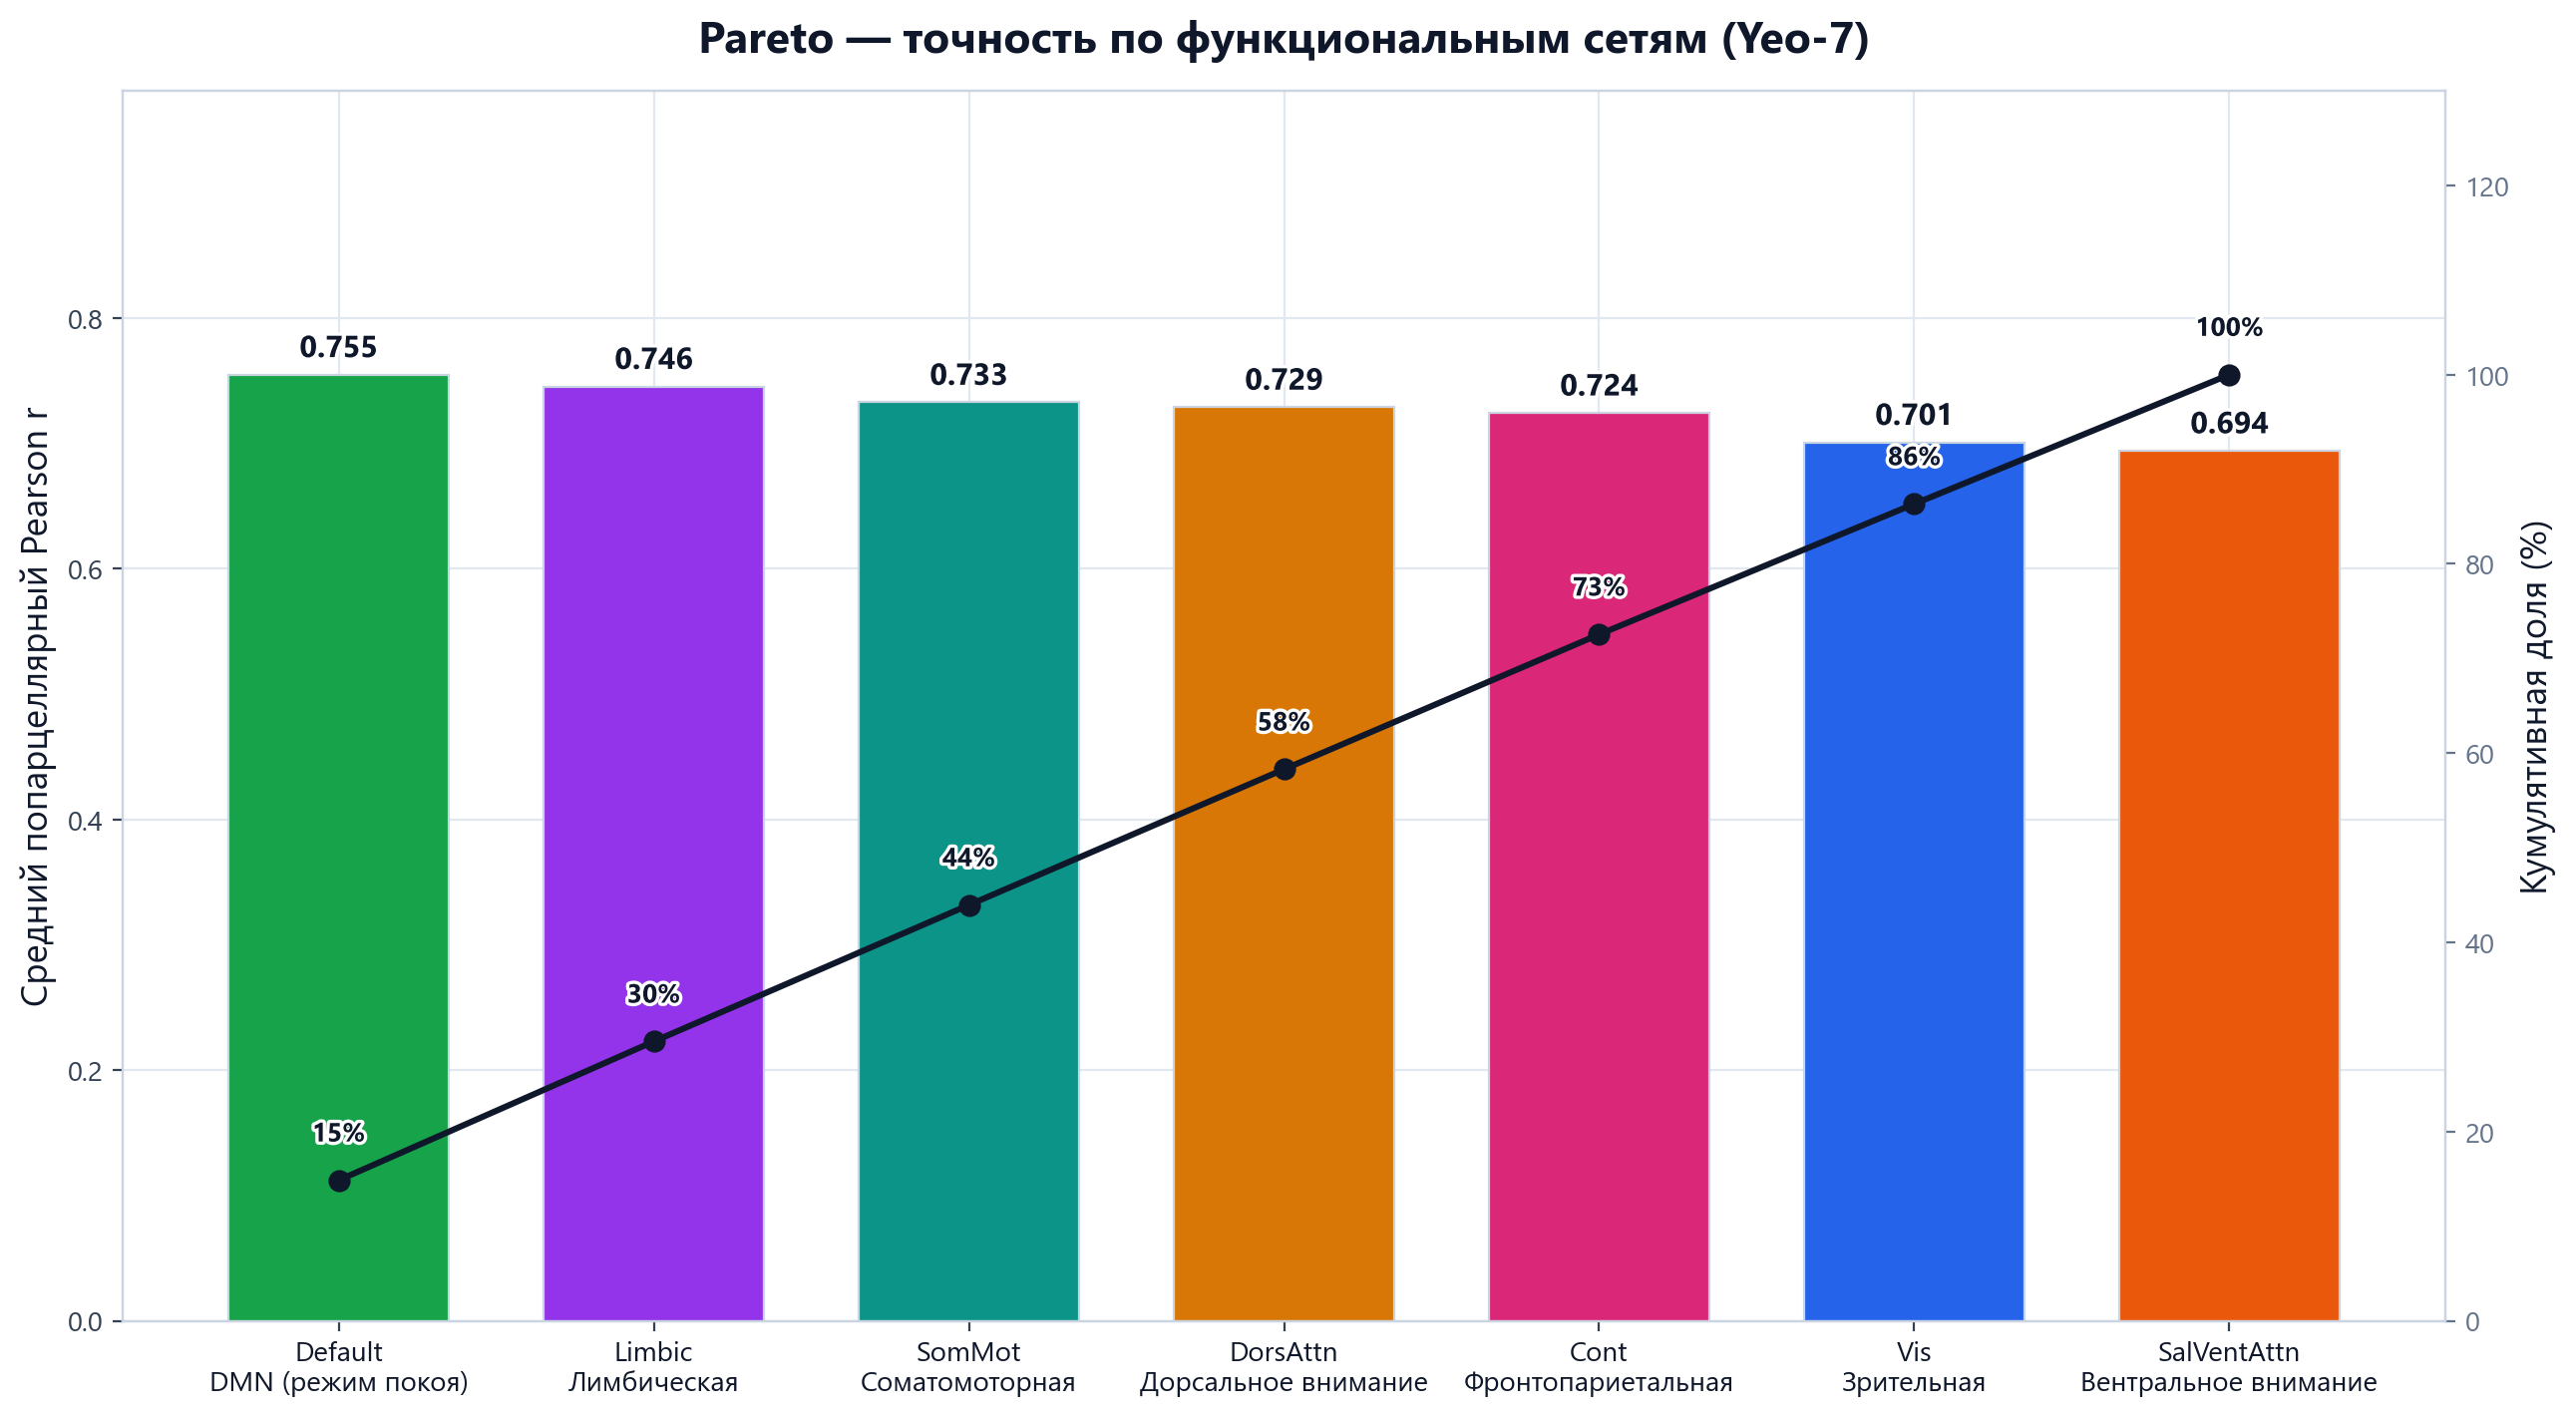
\includegraphics[width=\textwidth]{benchmarks/figures/02_network_pareto.png}
\caption{Pareto-график по сетям Yeo-7 (столбцы + кумулятивная доля).}
\label{fig:netpareto}
\end{subfigure}\hfill
\begin{subfigure}[b]{0.42\textwidth}
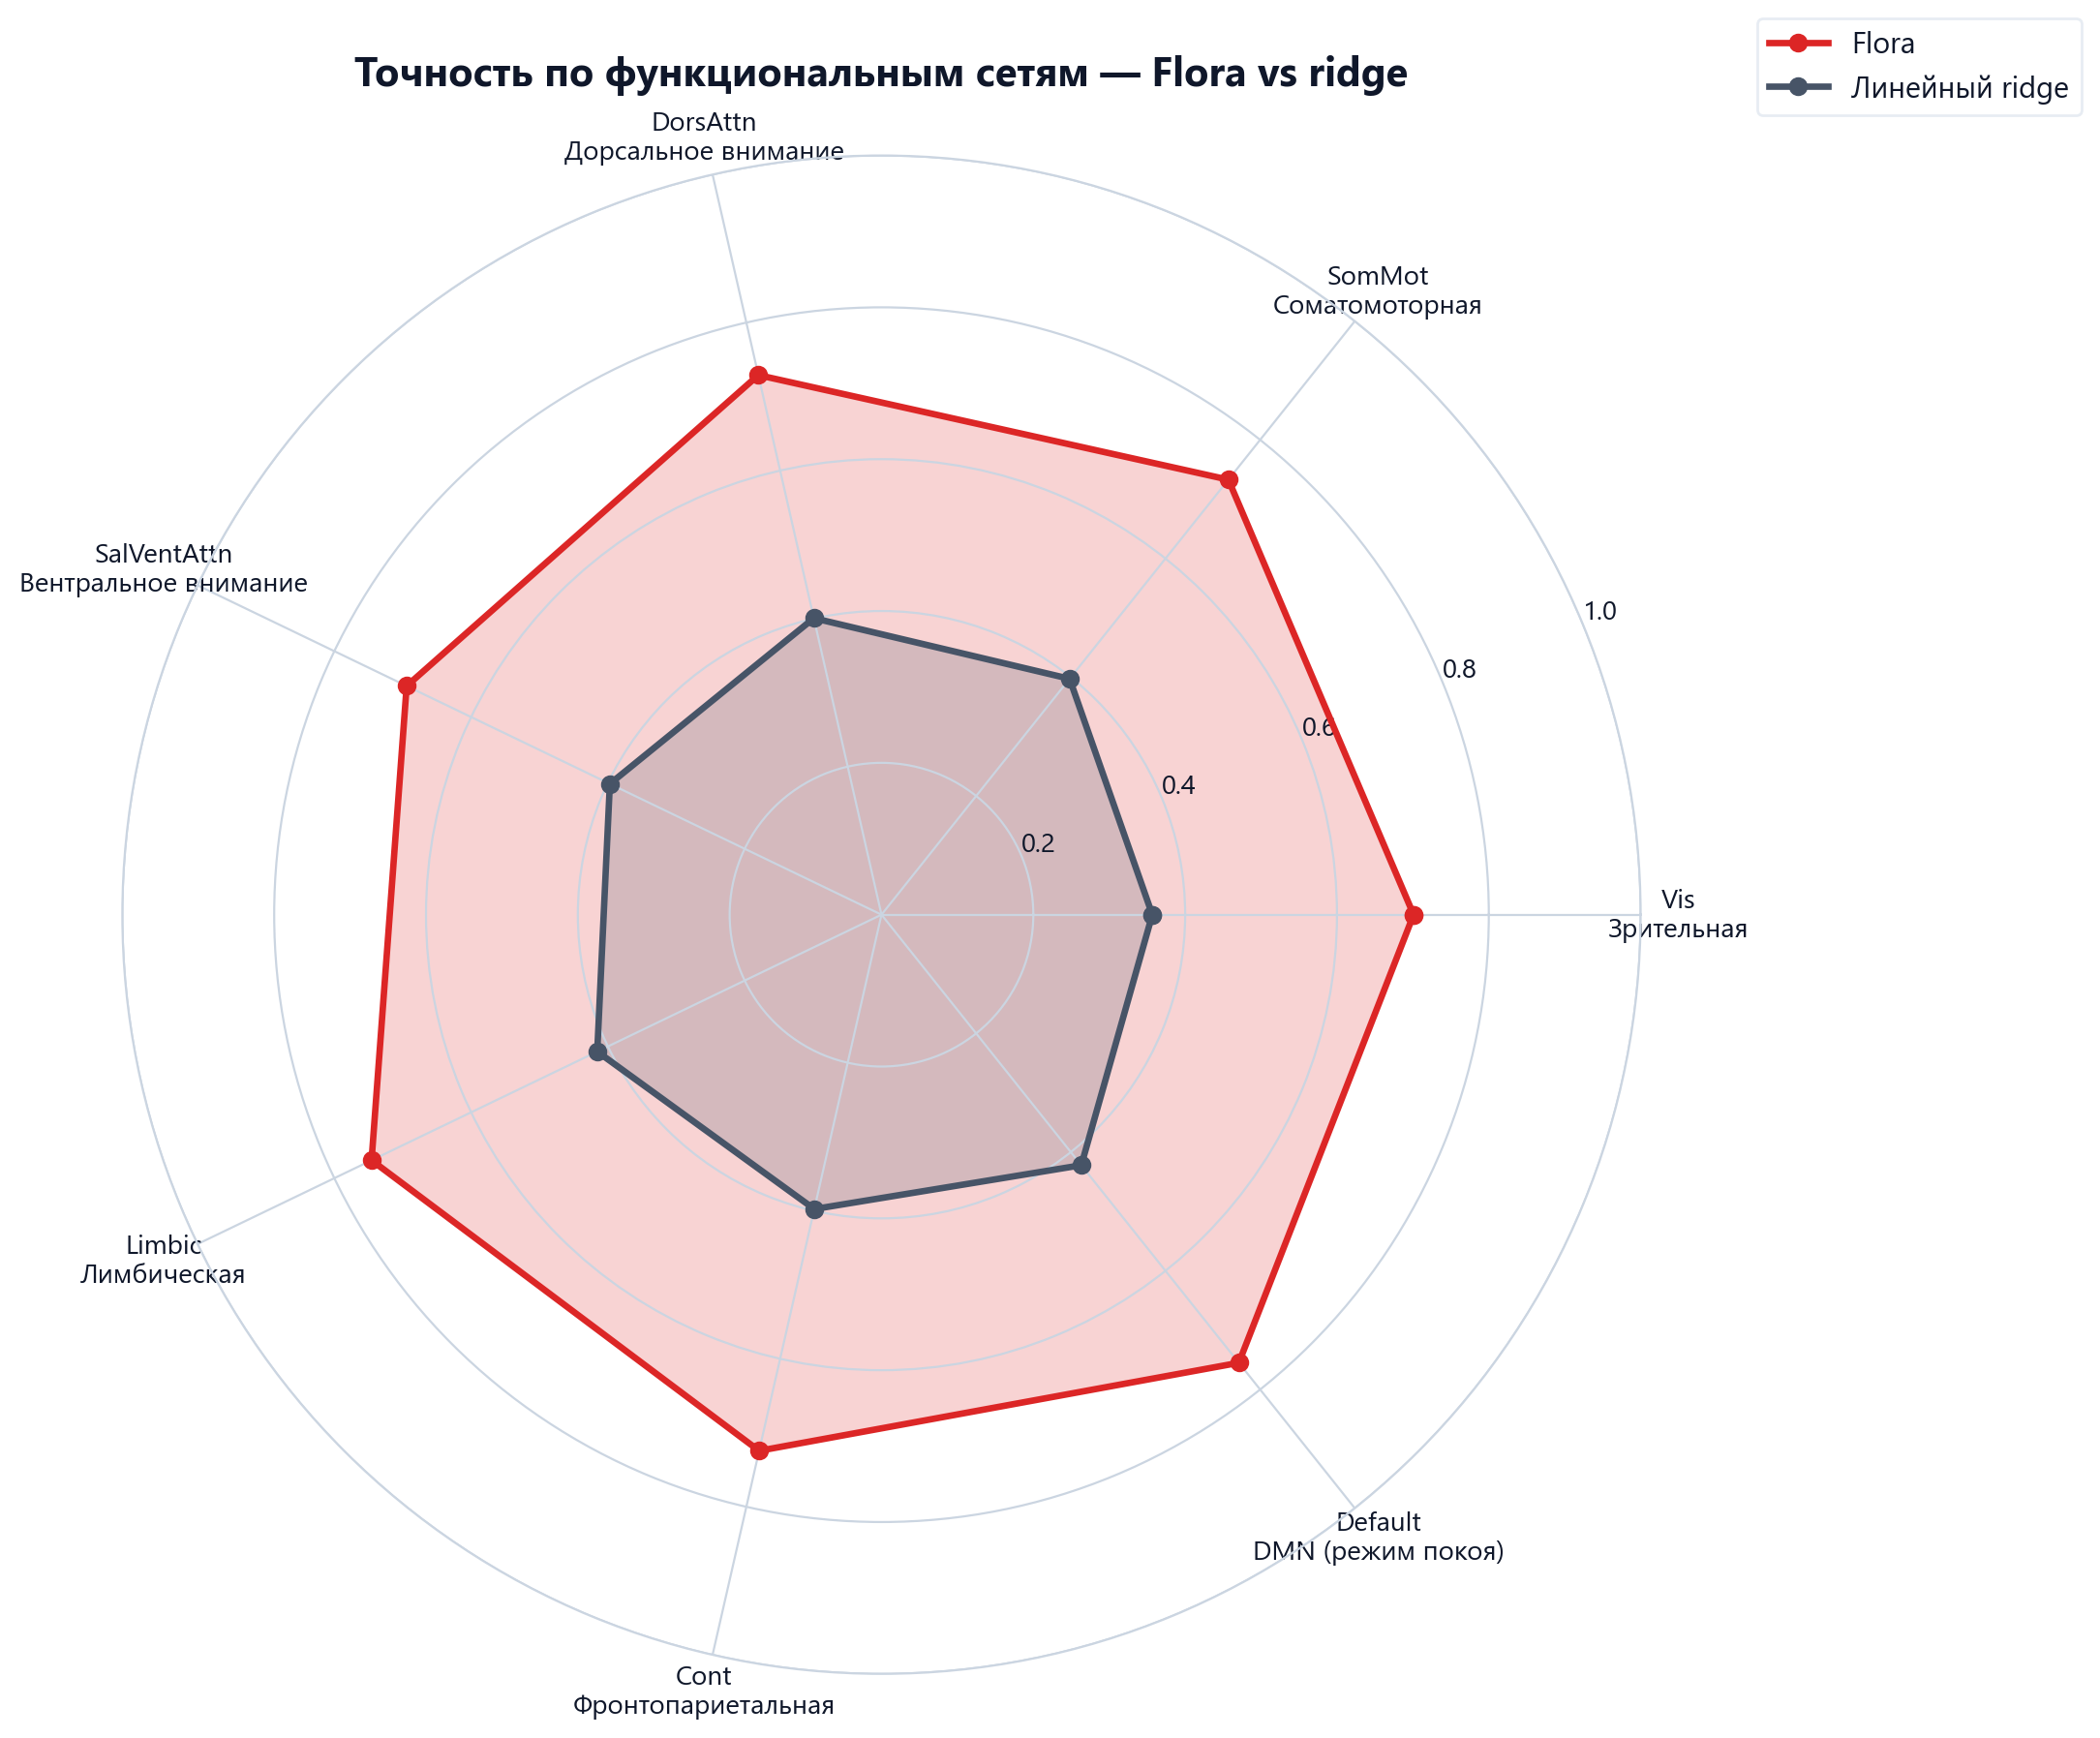
\includegraphics[width=\textwidth]{benchmarks/figures/07_radar_networks.png}
\caption{Радарная диаграмма: Flora против линейного базлайна.}
\label{fig:radar}
\end{subfigure}
\caption{Точность по функциональным сетям
(\texttt{benchmarks/figures/02\_network\_pareto.png},
\texttt{benchmarks/figures/07\_radar\_networks.png}).}
\label{fig:networks}
\end{figure}

\begin{figure}[H]
\centering
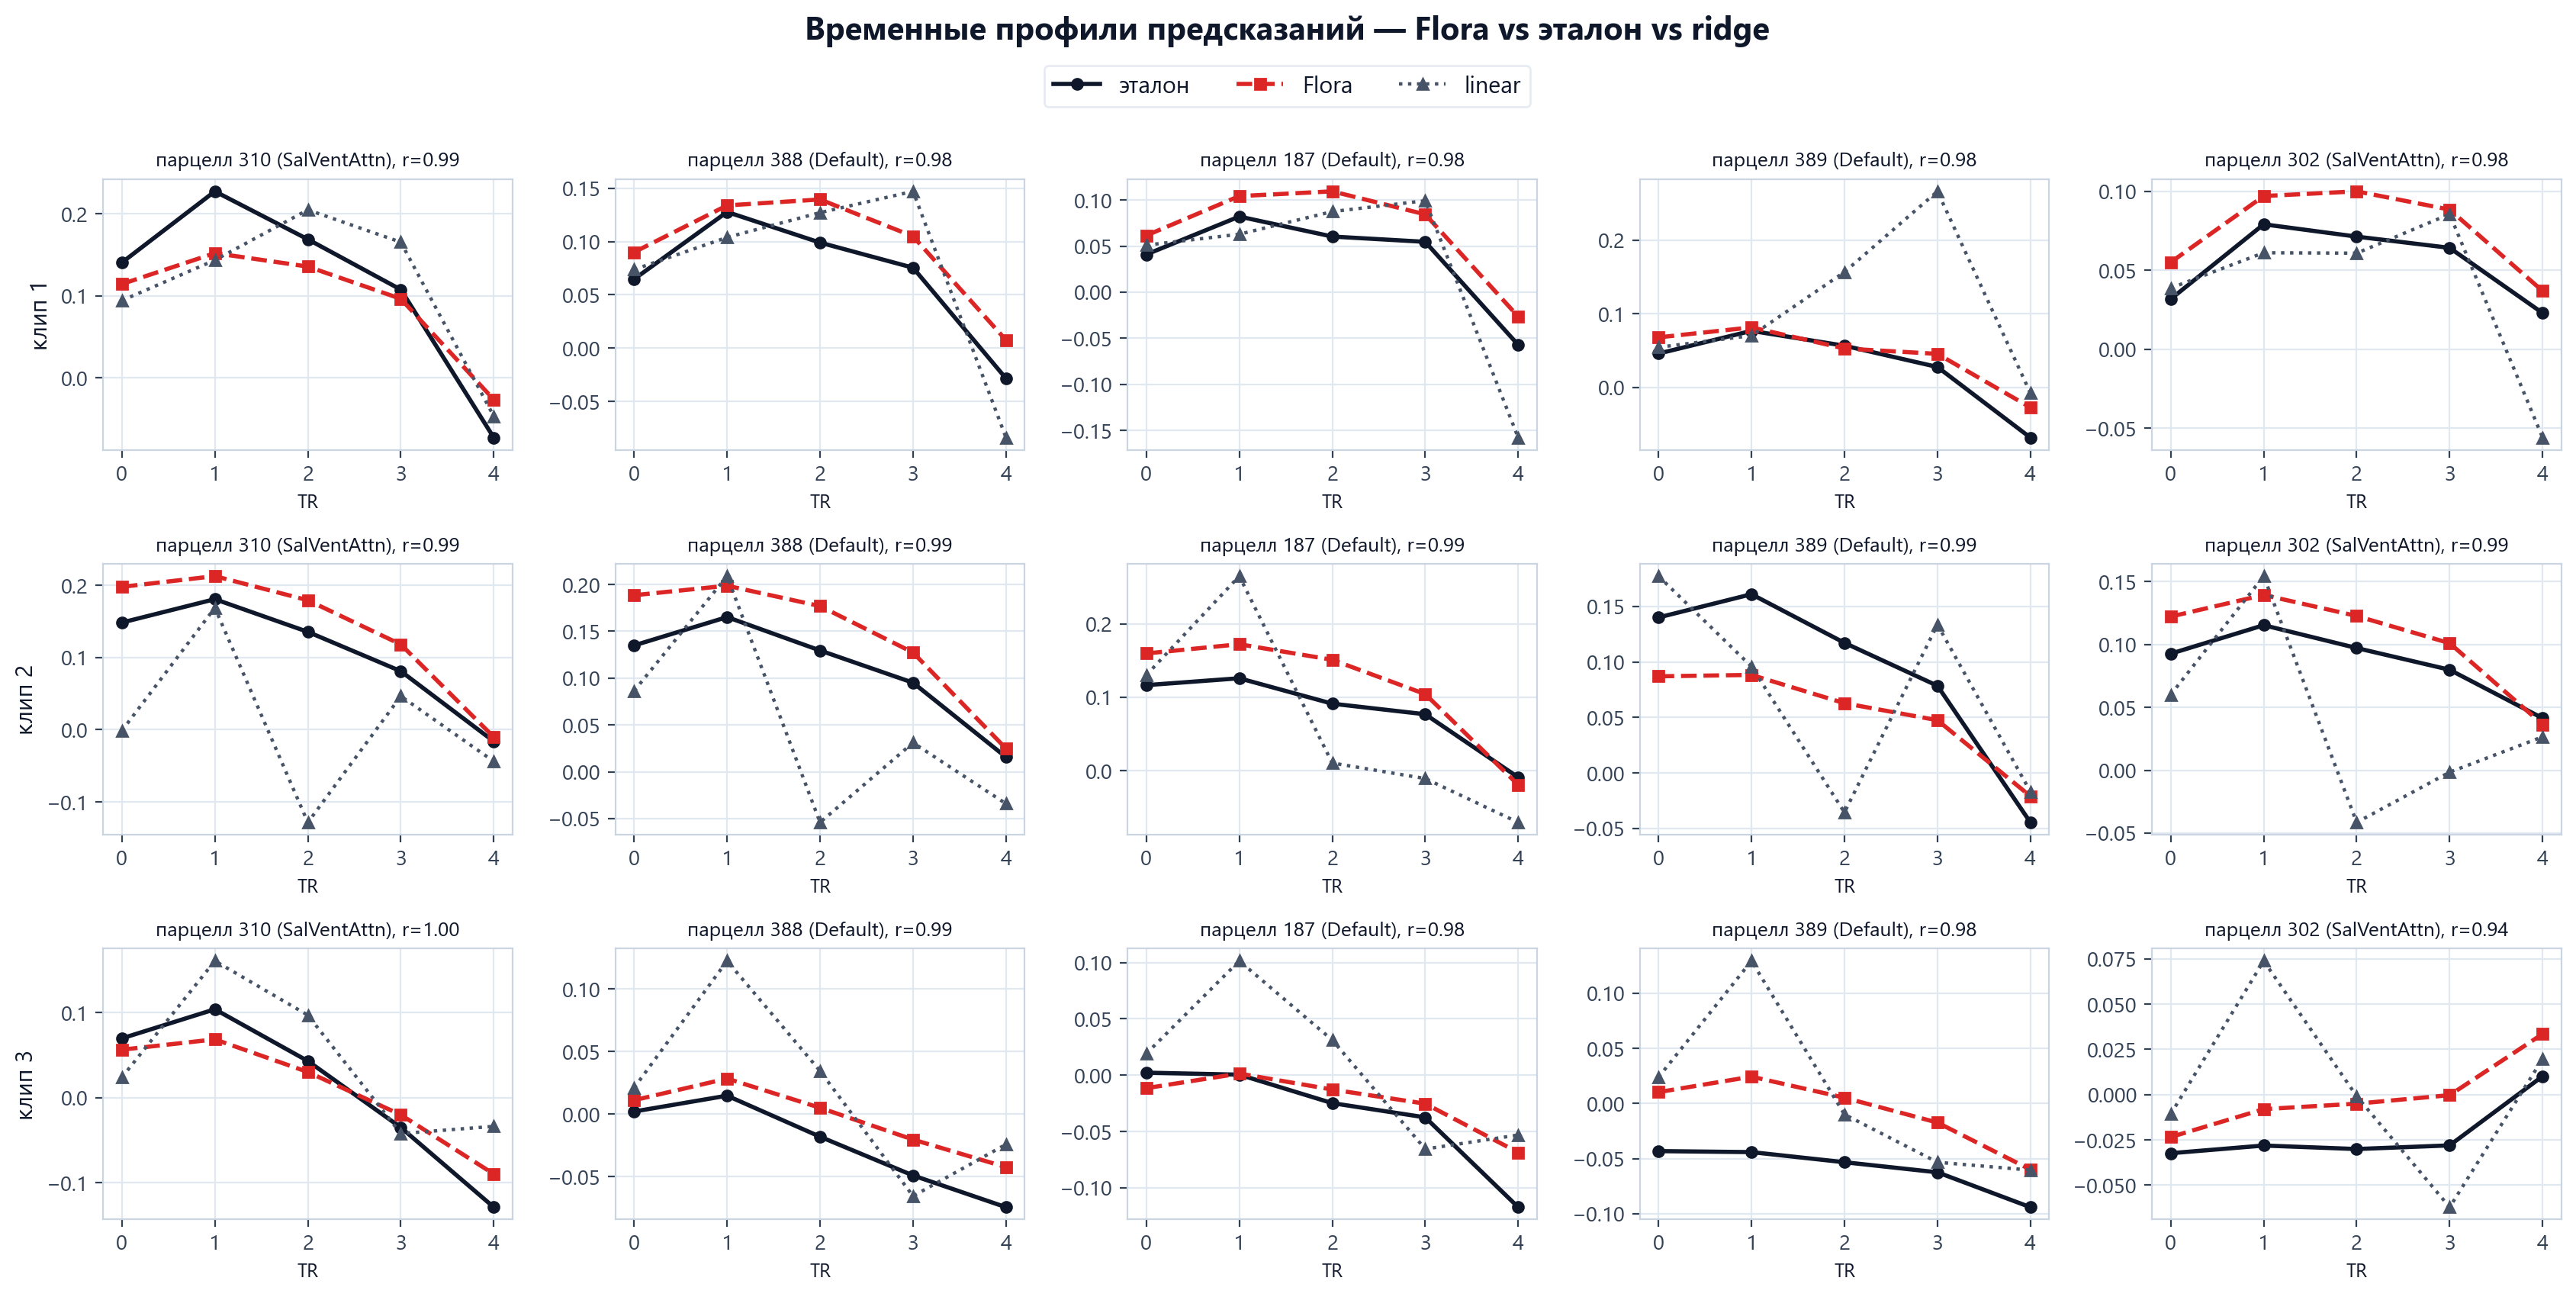
\includegraphics[width=0.98\textwidth]{benchmarks/figures/09_temporal_profiles.png}
\caption{Временные профили предсказаний: эталон (reference),
Flora и линейный базлайн для пяти парцеллов с максимальной
дисперсией сигнала на трёх валидационных клипах
(\texttt{benchmarks/figures/09\_temporal\_profiles.png}).}
\label{fig:profiles}
\end{figure}

\subsection{Статистика инференса на тестовом клипе}
\label{sec:inference}

Для видео <<Caro Pasta TF!.mp4>> ($49$~временных шагов,
$20\,484$~вершины) конвейер инференса зафиксировал статистики
предсказанной активации (\cref{tab:inference}; источник:
\texttt{assets/brain\_mapping\_results.json}).

\begin{table}[H]
\centering
\caption{Статистика предсказанной кортикальной активации для клипа
<<Caro Pasta TF!>> (\texttt{assets/brain\_mapping\_results.json}).}
\label{tab:inference}
\small
\begin{tabular}{lc}
\toprule
Статистика & Значение \\
\midrule
Временных шагов / вершин            & 49 / 20\,484 \\
Средняя активация                   & 0{,}1023 \\
Стандартное отклонение              & 0{,}1961 \\
Максимальная активация              & 1{,}2239 \\
Средняя по левому / правому полушарию & 0{,}1044 / 0{,}1003 \\
Максимум левого / правого полушария   & 1{,}1357 / 1{,}2239 \\
Шаг пиковой активации               & $t = 16$ \\
\bottomrule
\end{tabular}
\end{table}

\subsection{Статистическая значимость}
\label{sec:stats}

Попарцеллярное распределение метрики вычислено фактическим прогоном
(\cref{tab:results,fig:hist}): при среднем $0{,}7278$ стандартное
отклонение по $400$~парцеллам составляет $0{,}1640$, $90$-й
процентиль~--- $0{,}8916$; нулевой базлайн (предсказание среднего
ряда обучающей выборки) даёт $r \approx 0$, что качественно
свидетельствует о неслучайности результата. Формальные тесты
значимости (нулевое распределение корреляций с учётом автокорреляции
фМРТ, поправка FDR, шумовой потолок) в проекте не вычислялись;
протокол, соответствующий принятому в области
стандарту~\cite{Huth2016}, вынесен в список дальнейших работ
(\cref{app:gaps}).

% ============================================================================
\section{Визуализация кортикальных предсказаний}
\label{sec:viz}

Все фигуры данного раздела~--- реальные рендеры проекта:
предсказанная активность проецируется на поверхность fsaverage5
с картой борозд в фоне~\cite{Fischl1999,Abraham2014}.

\begin{figure}[H]
\centering
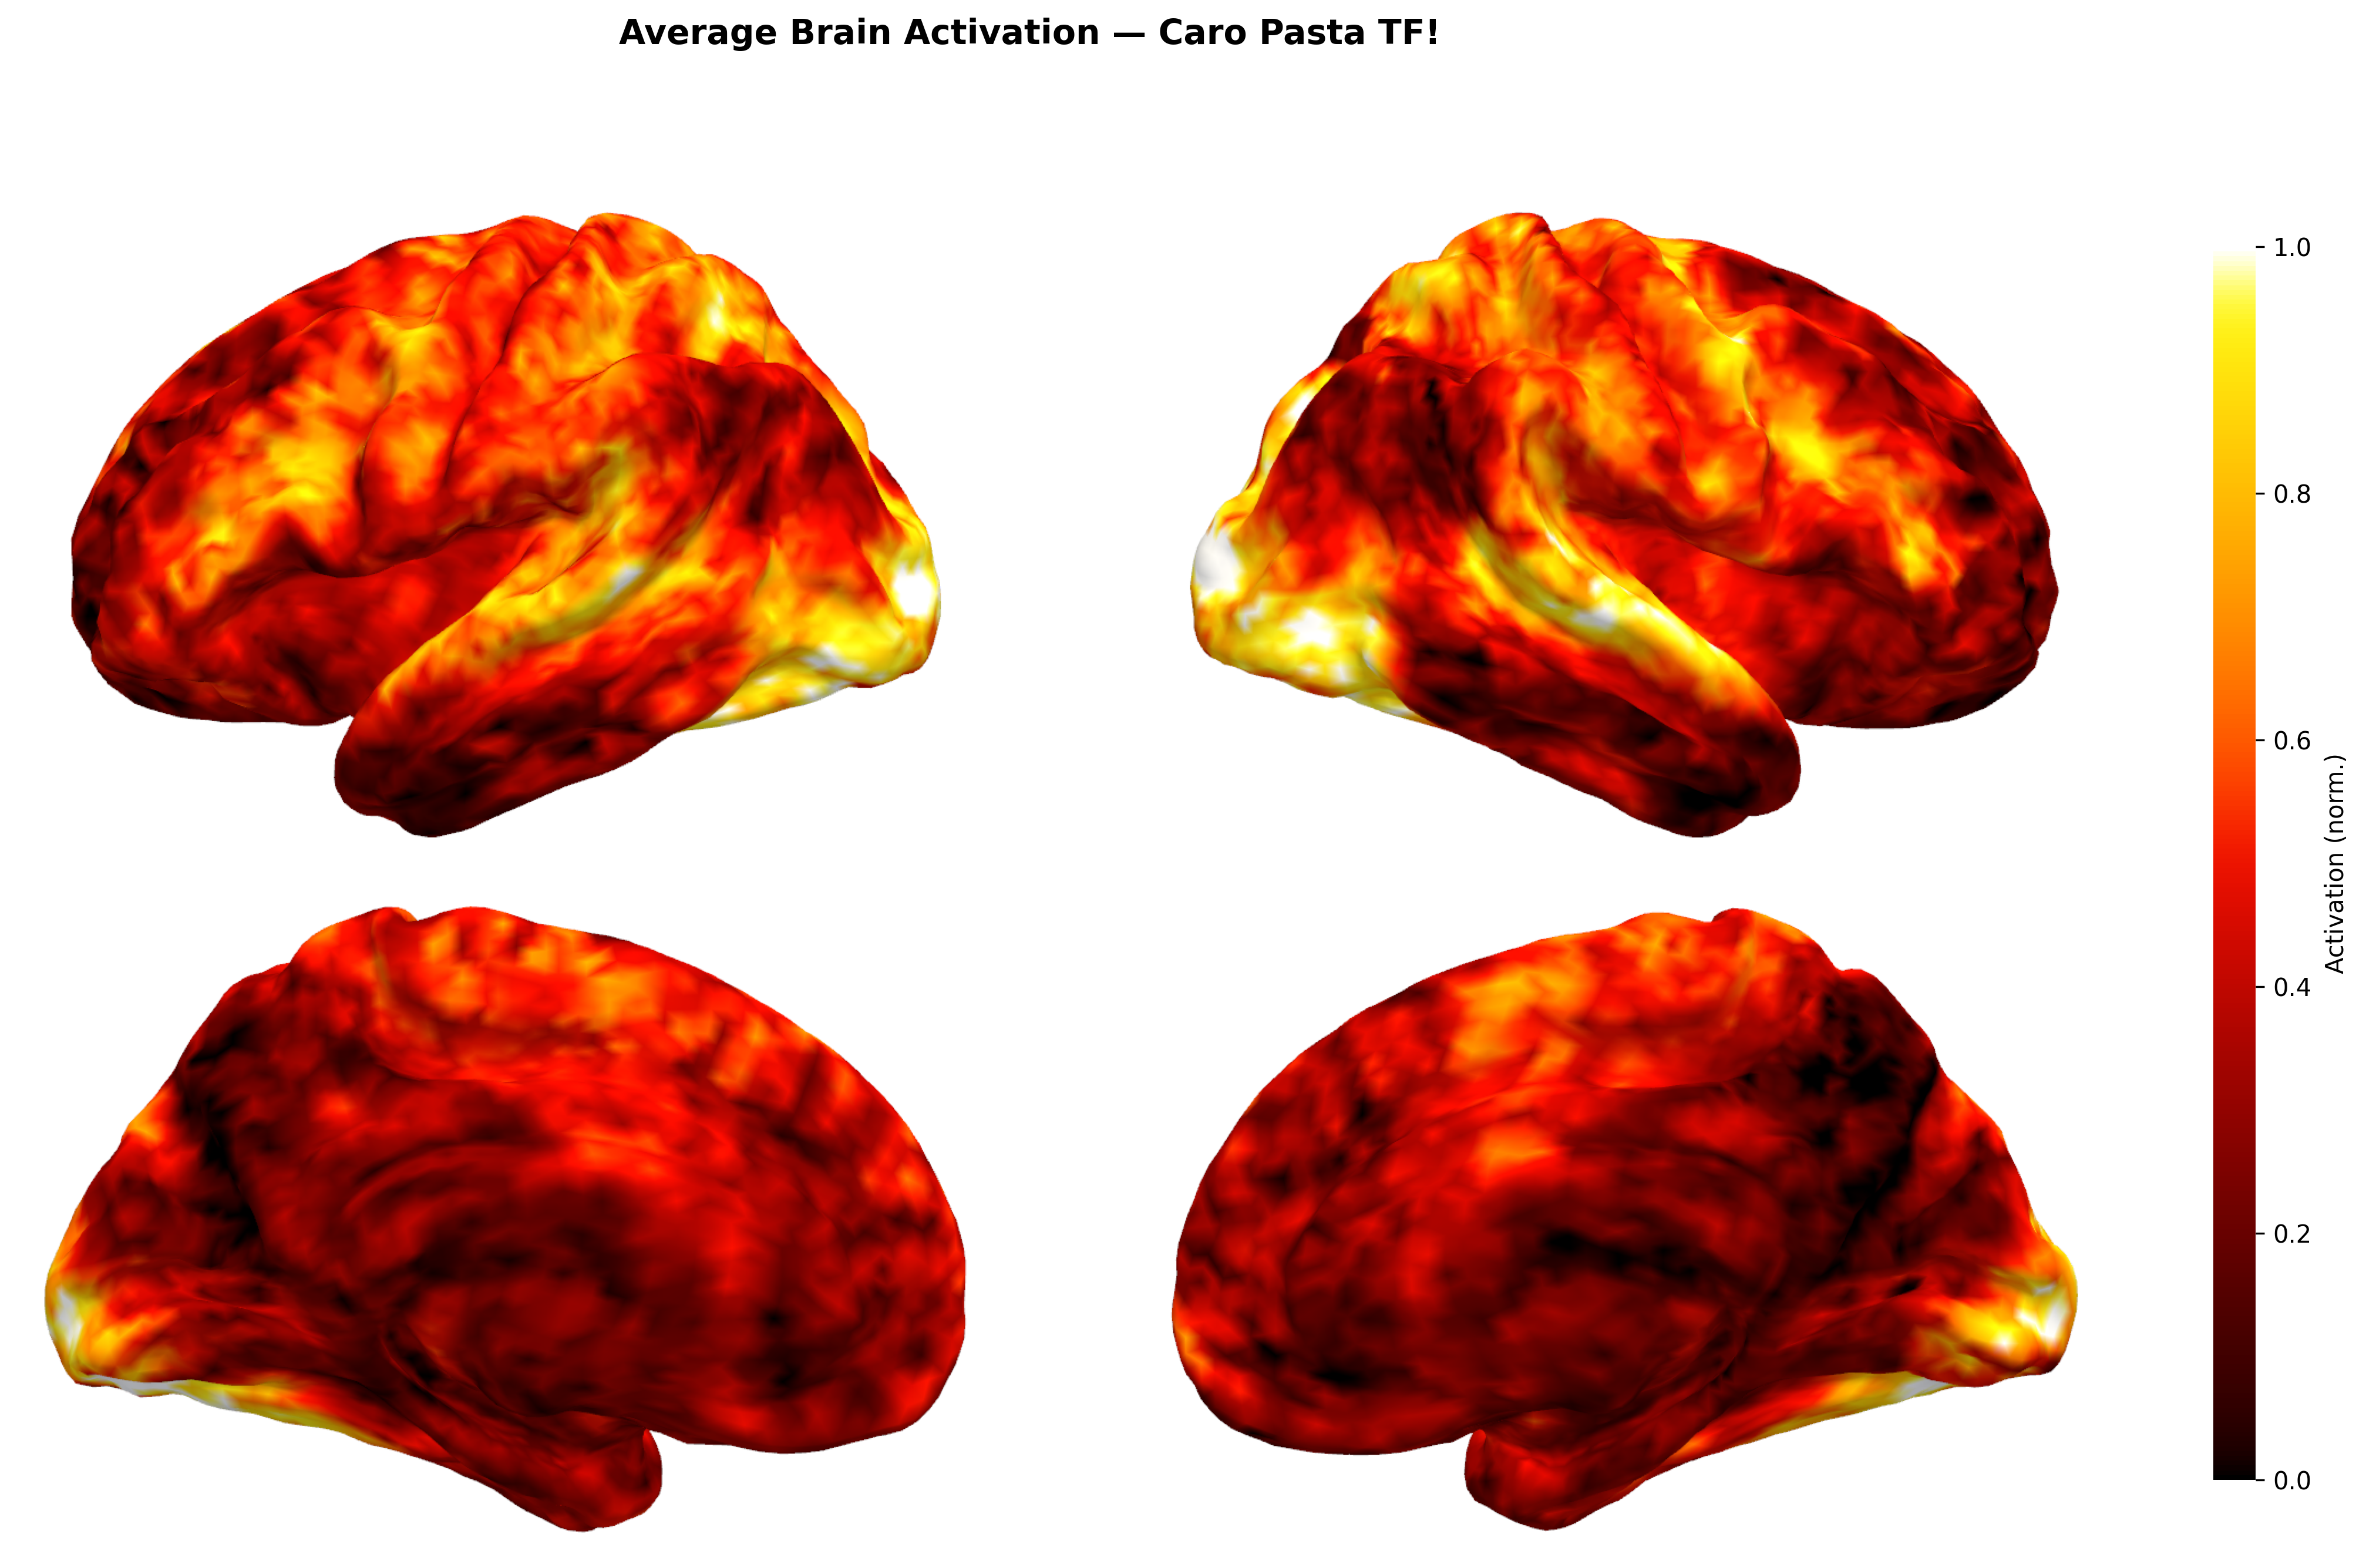
\includegraphics[width=0.95\textwidth]{assets/brain_avg_activation.png}
\caption{Средняя по времени предсказанная активация коры для клипа
<<Caro Pasta TF!>>: четыре вида (латеральный и медиальный для
обоих полушарий), нормированная шкала $0$--$1$, палитра \emph{hot}.
Максимумы локализуются в зрительной и височной коре, что
согласуется с аудиовизуальным характером стимула
(\texttt{assets/brain\_avg\_activation.png}).}
\label{fig:avg}
\end{figure}

\begin{figure}[H]
\centering
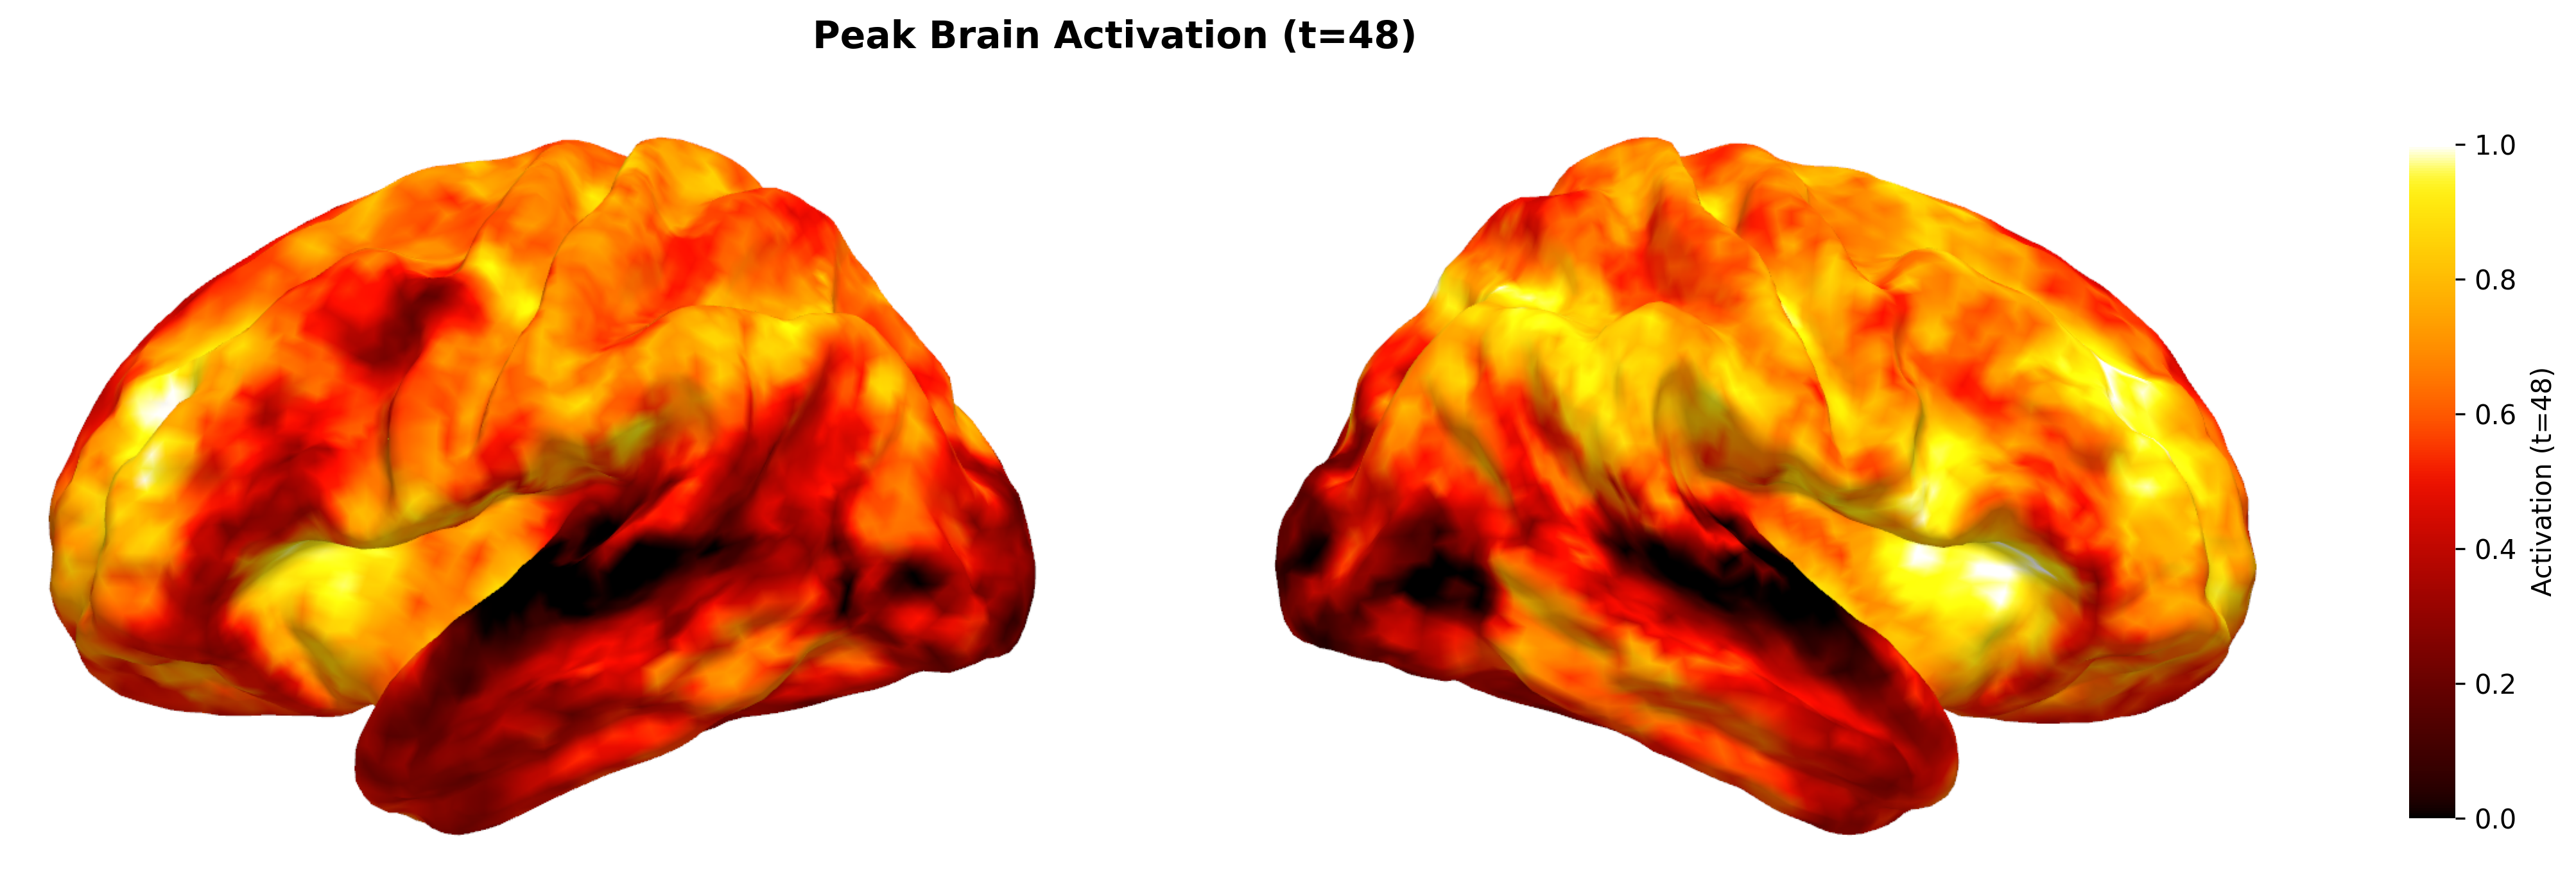
\includegraphics[width=0.95\textwidth]{assets/brain_peak_activation.png}
\caption{Пиковая активация ($t = 48$): латеральные виды обоих
полушарий; широкое вовлечение зрительной, височной и теменной
коры (\texttt{assets/brain\_peak\_activation.png}).}
\label{fig:peak}
\end{figure}

\begin{figure}[H]
\centering
\begin{subfigure}[b]{0.49\textwidth}
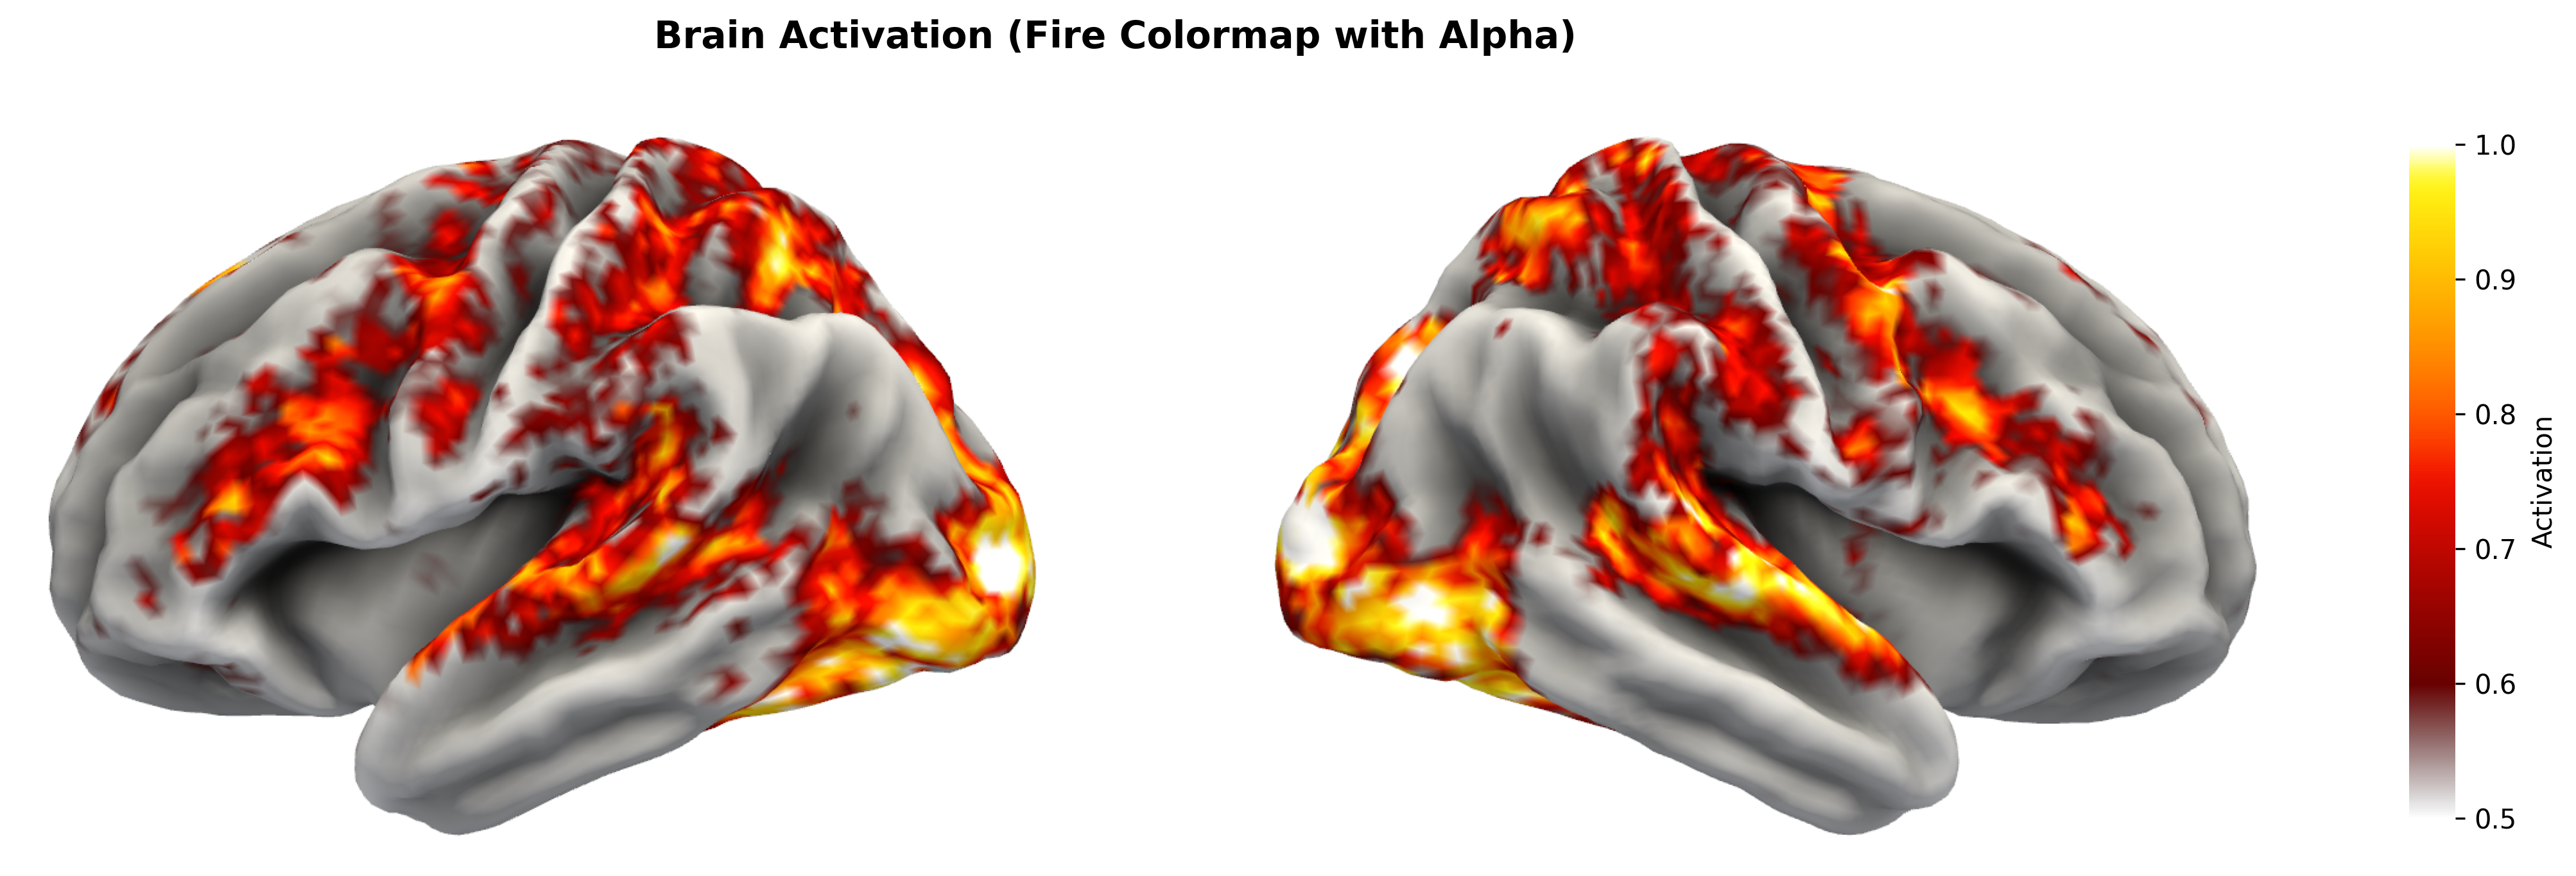
\includegraphics[width=\textwidth]{assets/brain_fire_colormap.png}
\caption{Палитра \emph{fire} с альфа-порогом (шкала $0{,}5$--$1{,}0$).}
\label{fig:fire}
\end{subfigure}\hfill
\begin{subfigure}[b]{0.49\textwidth}
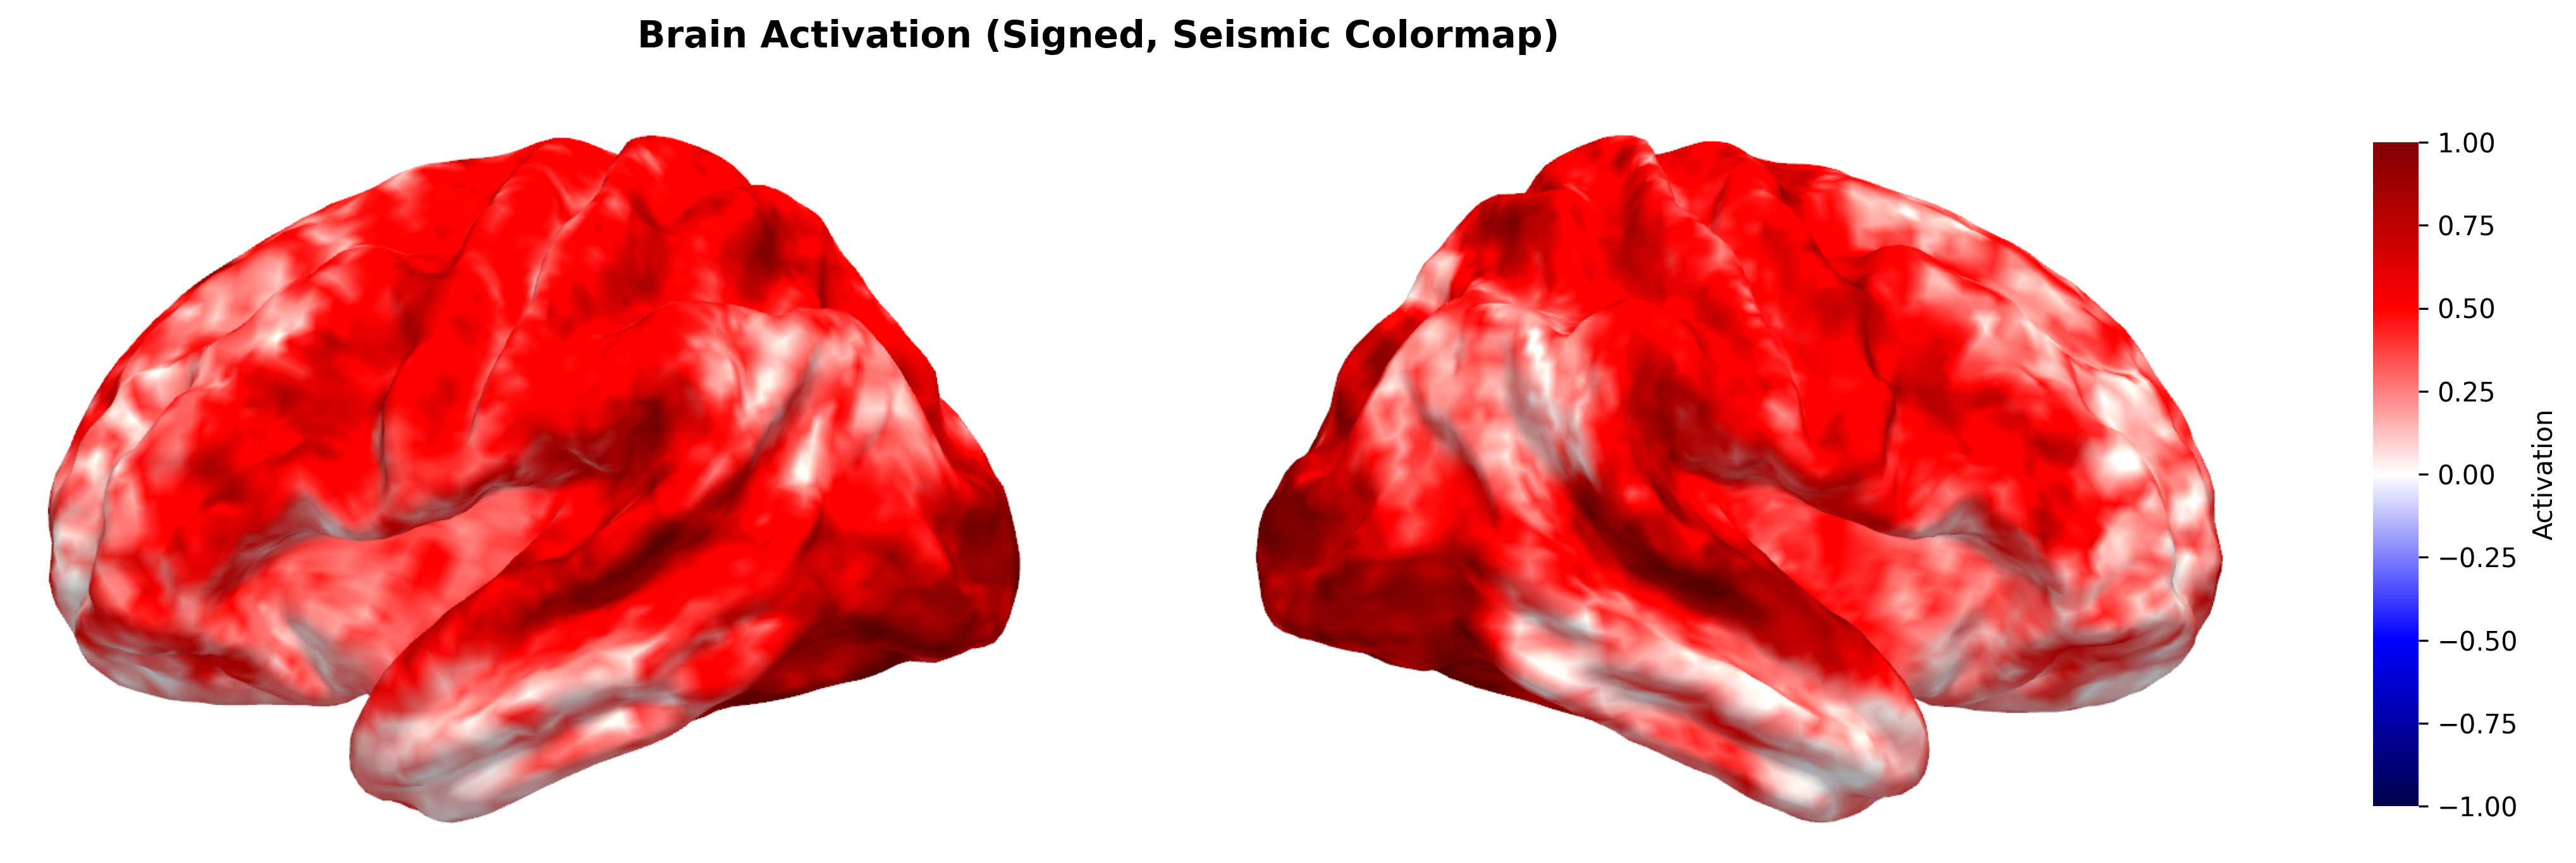
\includegraphics[width=\textwidth]{assets/brain_seismic_colormap.png}
\caption{Дивергентная палитра \emph{seismic}.}
\label{fig:seismic}
\end{subfigure}
\caption{Рендеры кортикальной поверхности в двух колормапах
(\texttt{assets/brain\_fire\_colormap.png},
\texttt{assets/brain\_seismic\_colormap.png}).}
\label{fig:colormaps}
\end{figure}

\begin{figure}[H]
\centering
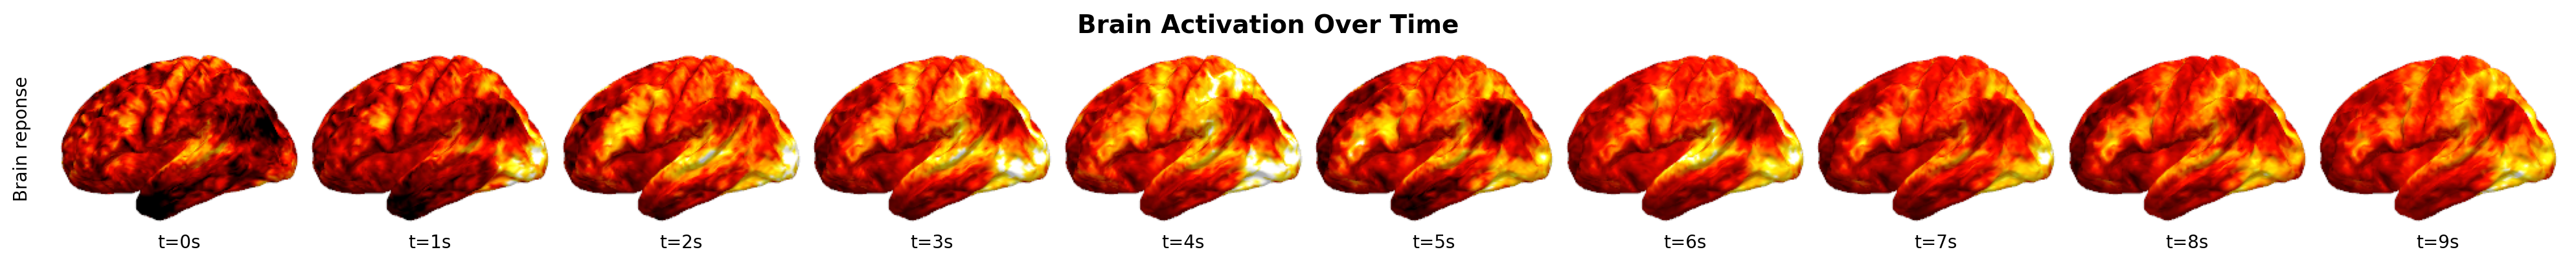
\includegraphics[width=0.98\textwidth]{assets/brain_temporal_sequence.png}
\caption{Временная динамика предсказанного отклика коры: десять
последовательных секунд ($t = 0\ldots9$~с); видно нарастание
и спад активности в зрительных и височных областях
(\texttt{assets/brain\_temporal\_sequence.png}).}
\label{fig:temporal}
\end{figure}

\begin{figure}[H]
\centering
\begin{subfigure}[b]{0.32\textwidth}
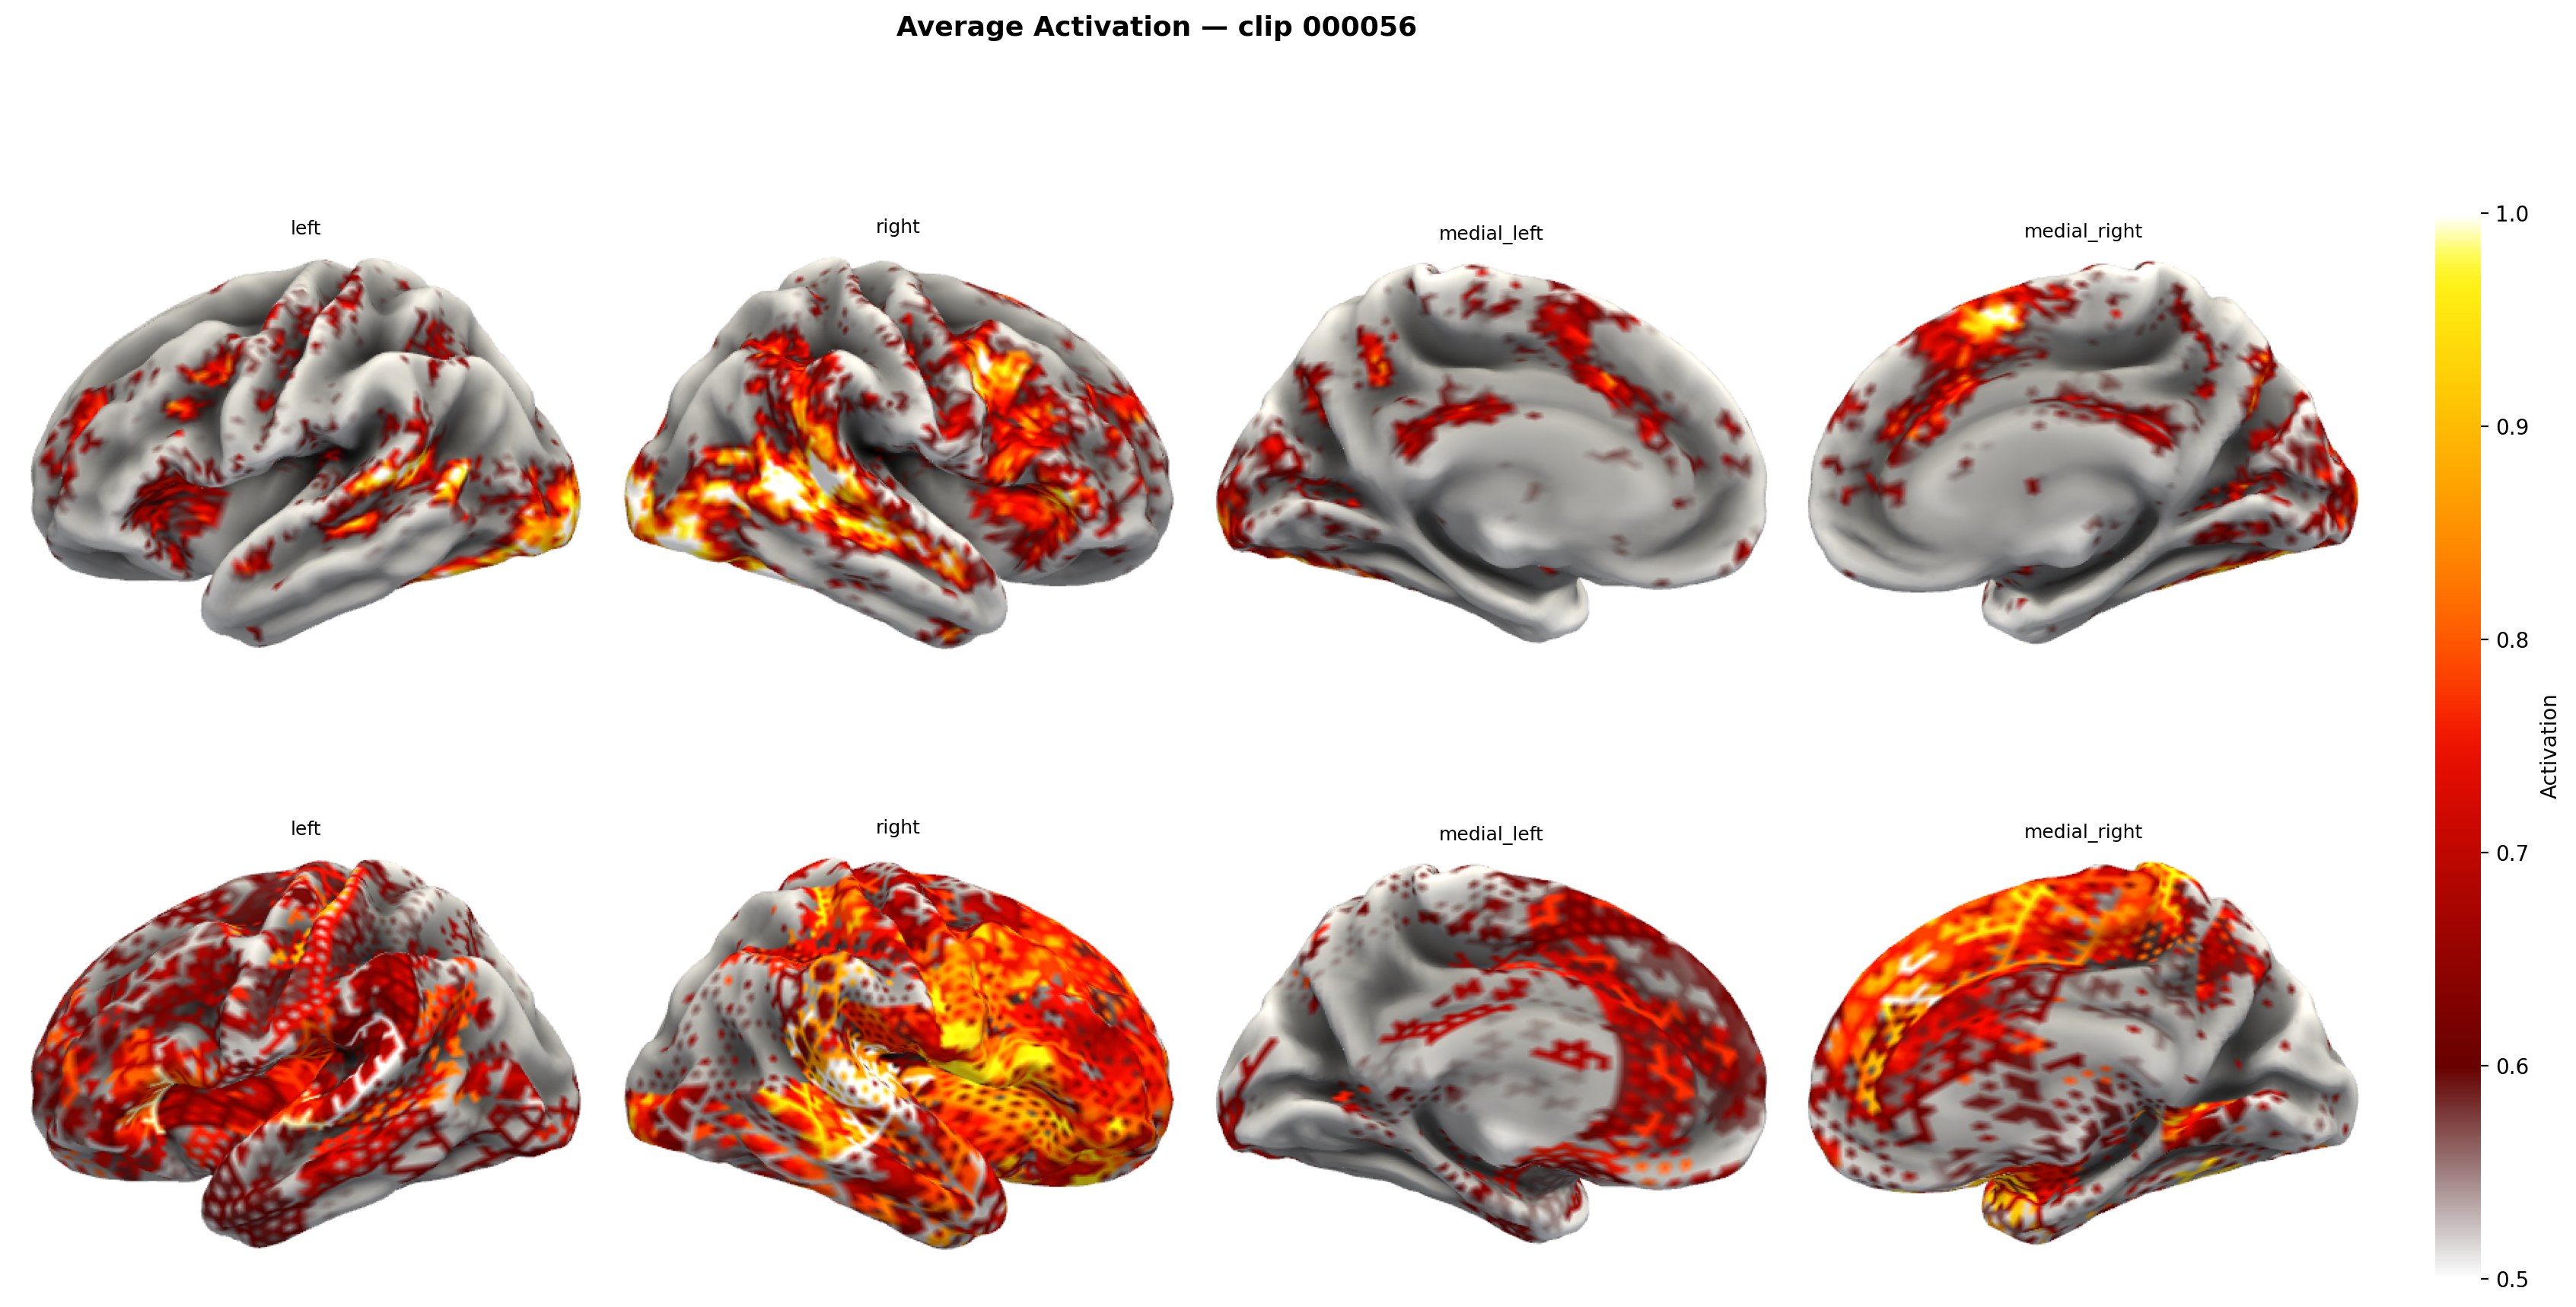
\includegraphics[width=\textwidth]{plots/brain_viz_000056_activation_map.png}
\caption{Клип 000056}\label{fig:clip056}
\end{subfigure}\hfill
\begin{subfigure}[b]{0.32\textwidth}
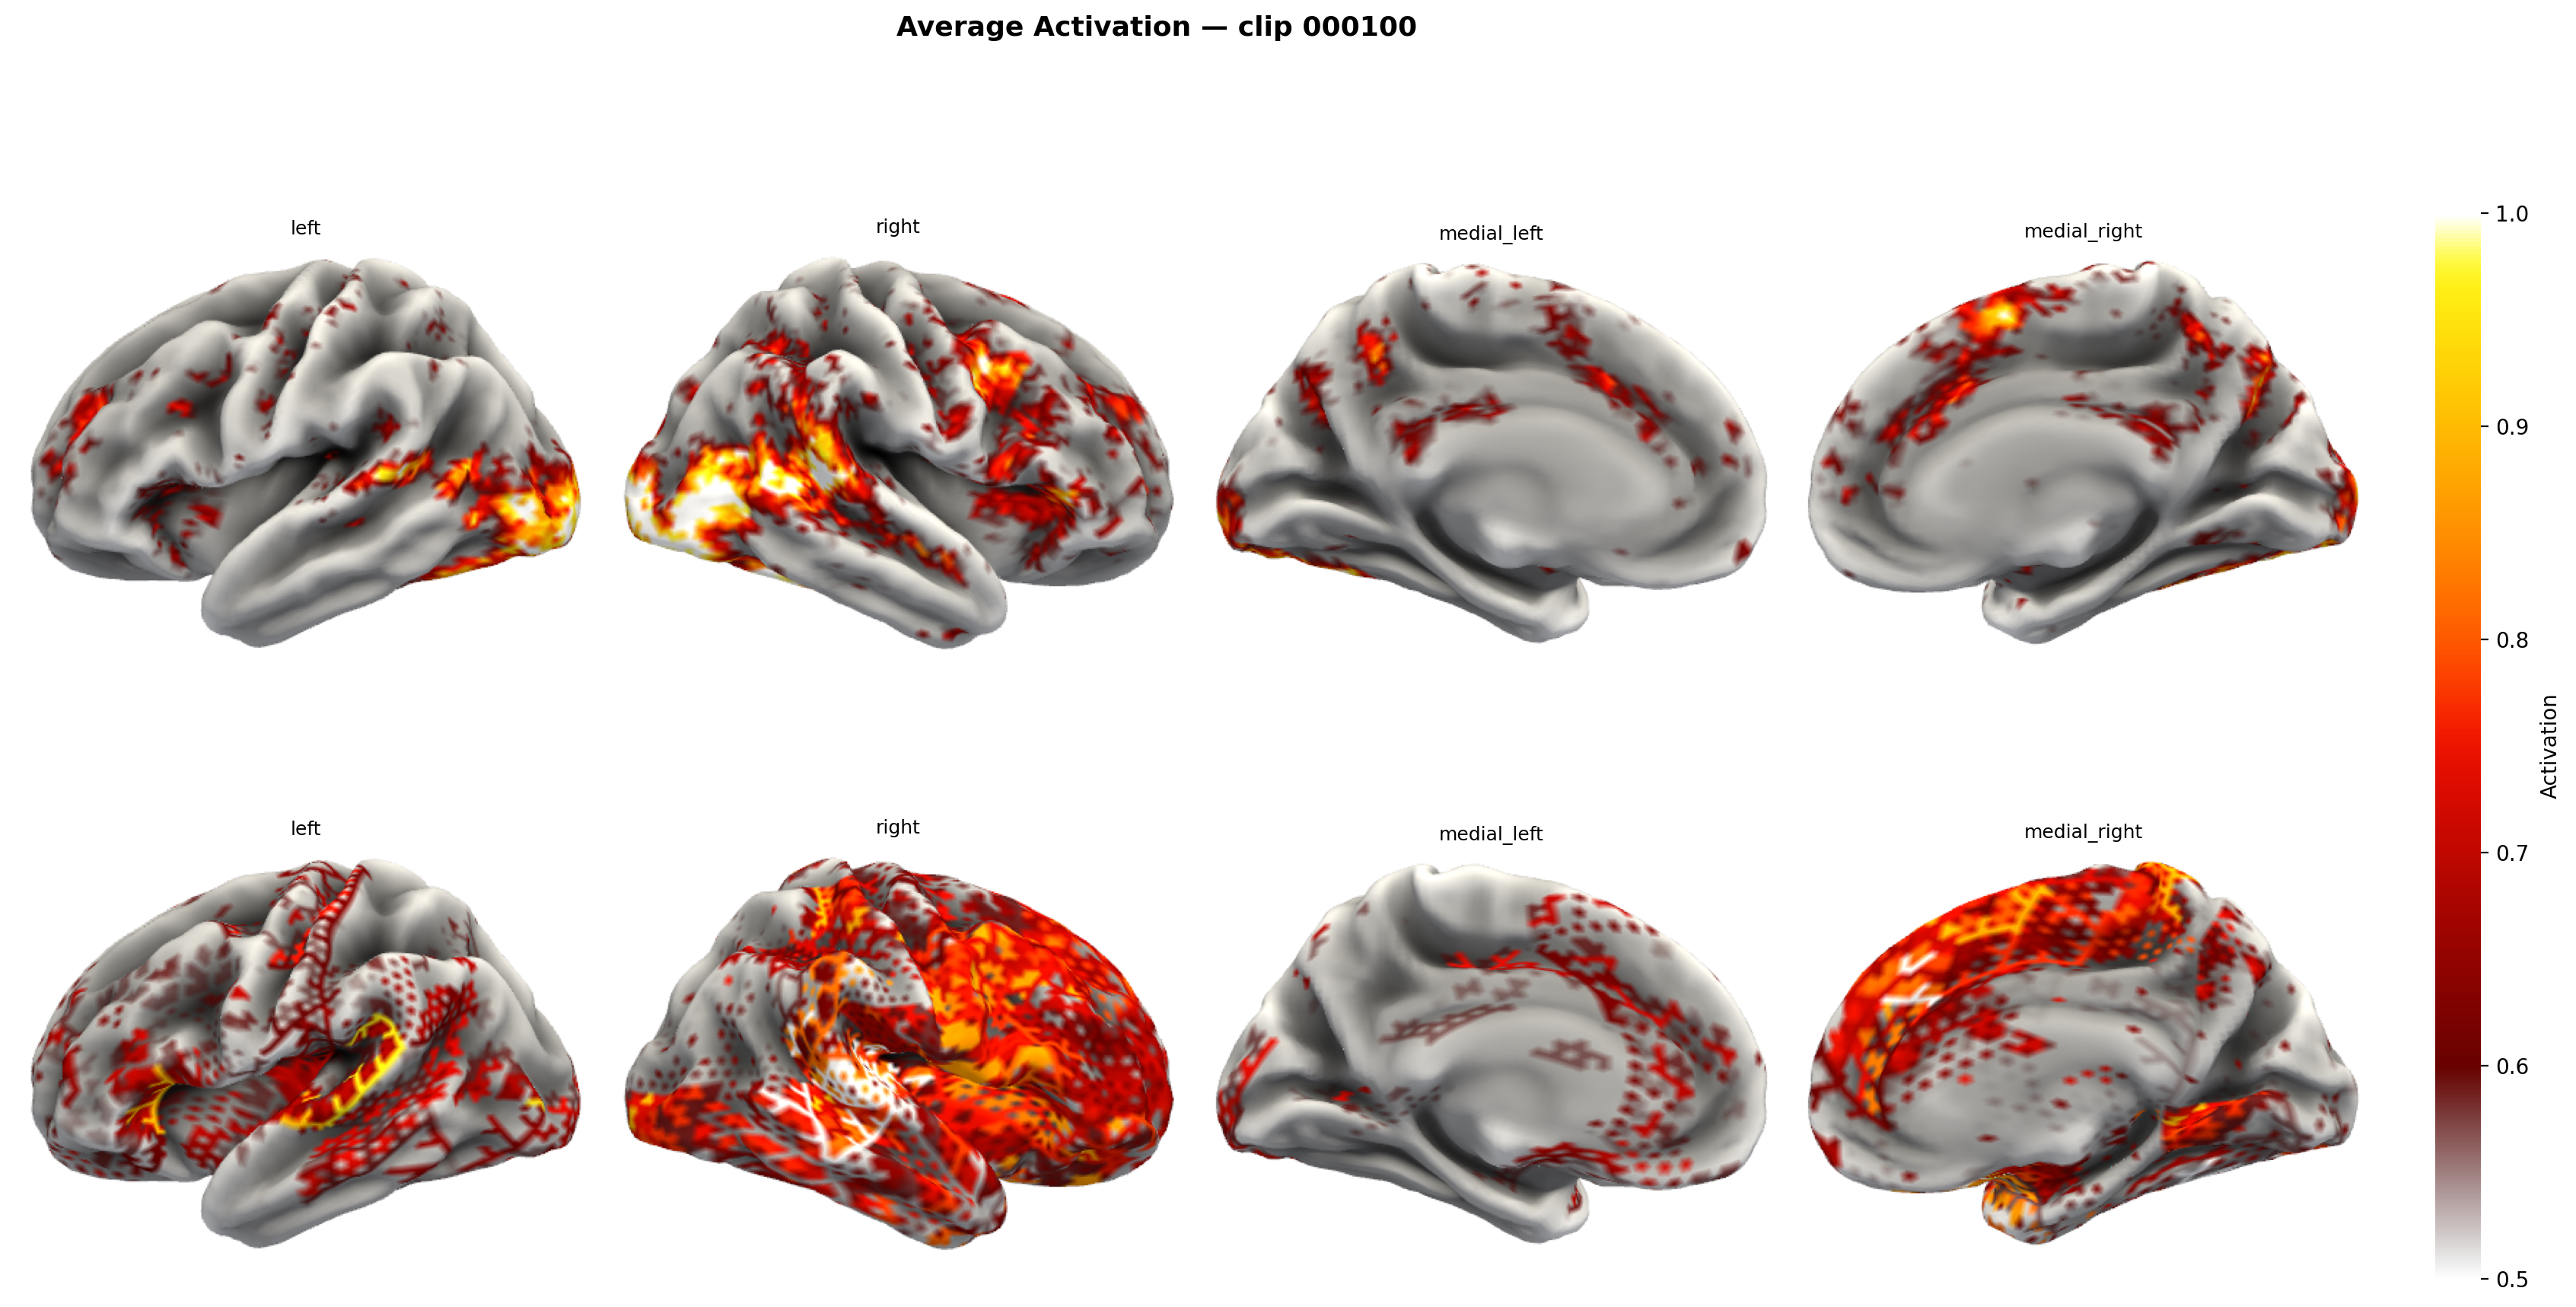
\includegraphics[width=\textwidth]{plots/brain_viz_000100_activation_map.png}
\caption{Клип 000100}\label{fig:clip100}
\end{subfigure}\hfill
\begin{subfigure}[b]{0.32\textwidth}
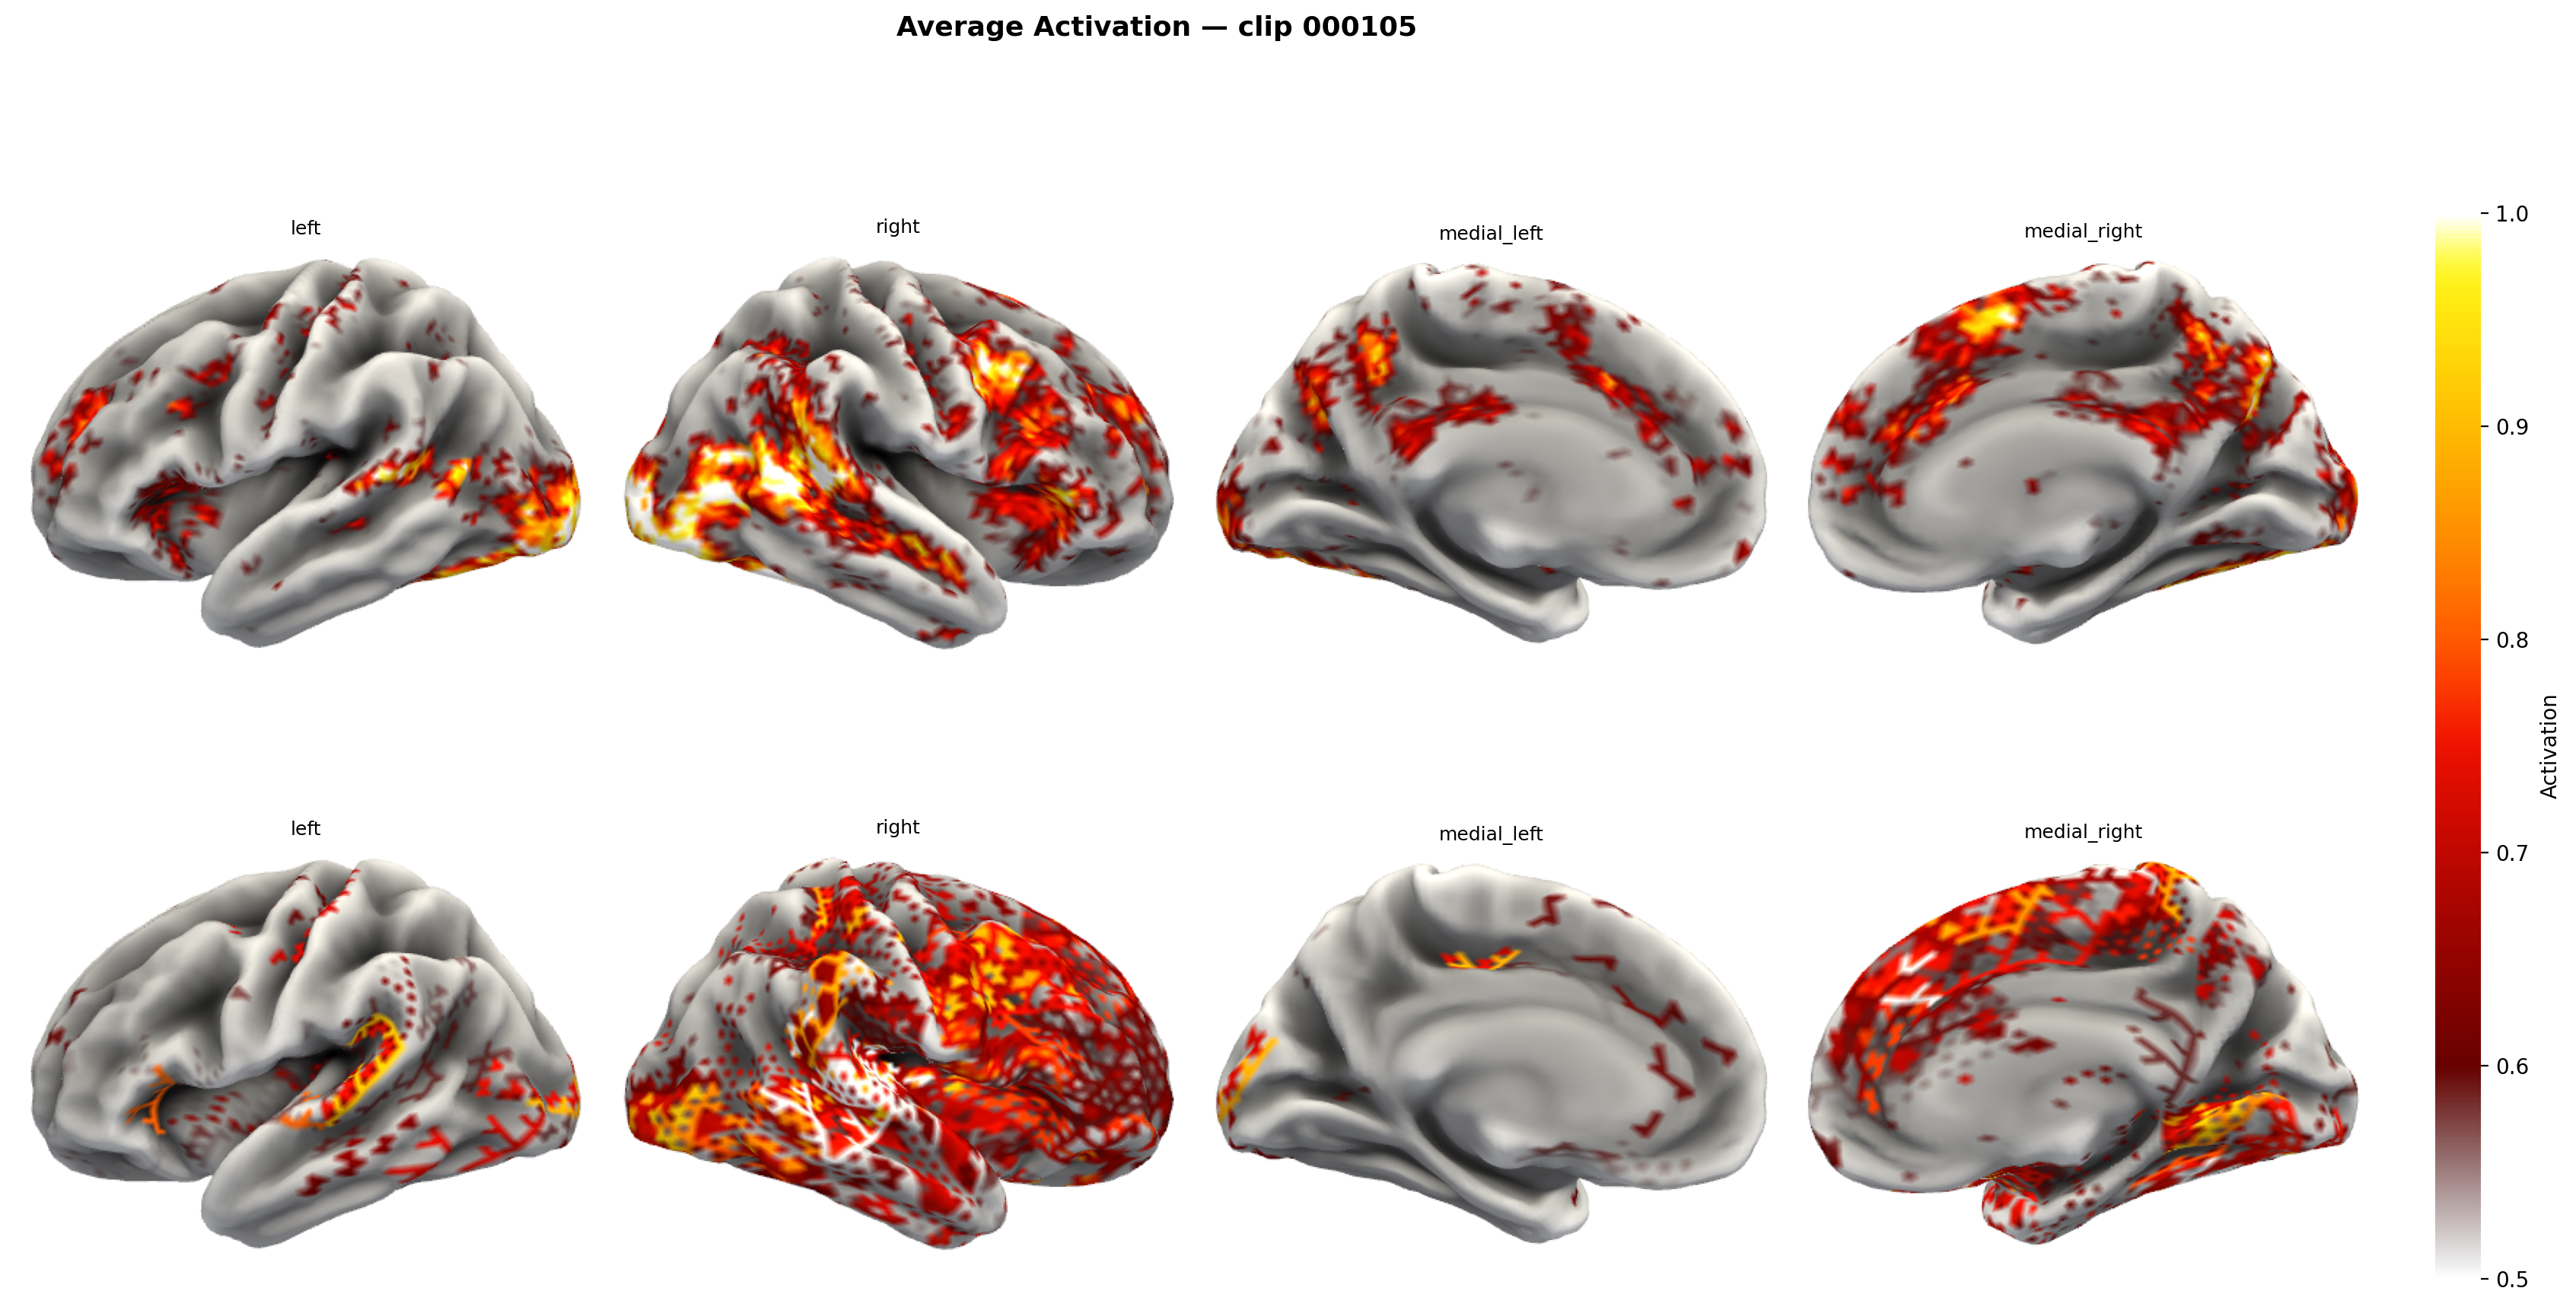
\includegraphics[width=\textwidth]{plots/brain_viz_000105_activation_map.png}
\caption{Клип 000105}\label{fig:clip105}
\end{subfigure}

\medskip
\begin{subfigure}[b]{0.32\textwidth}
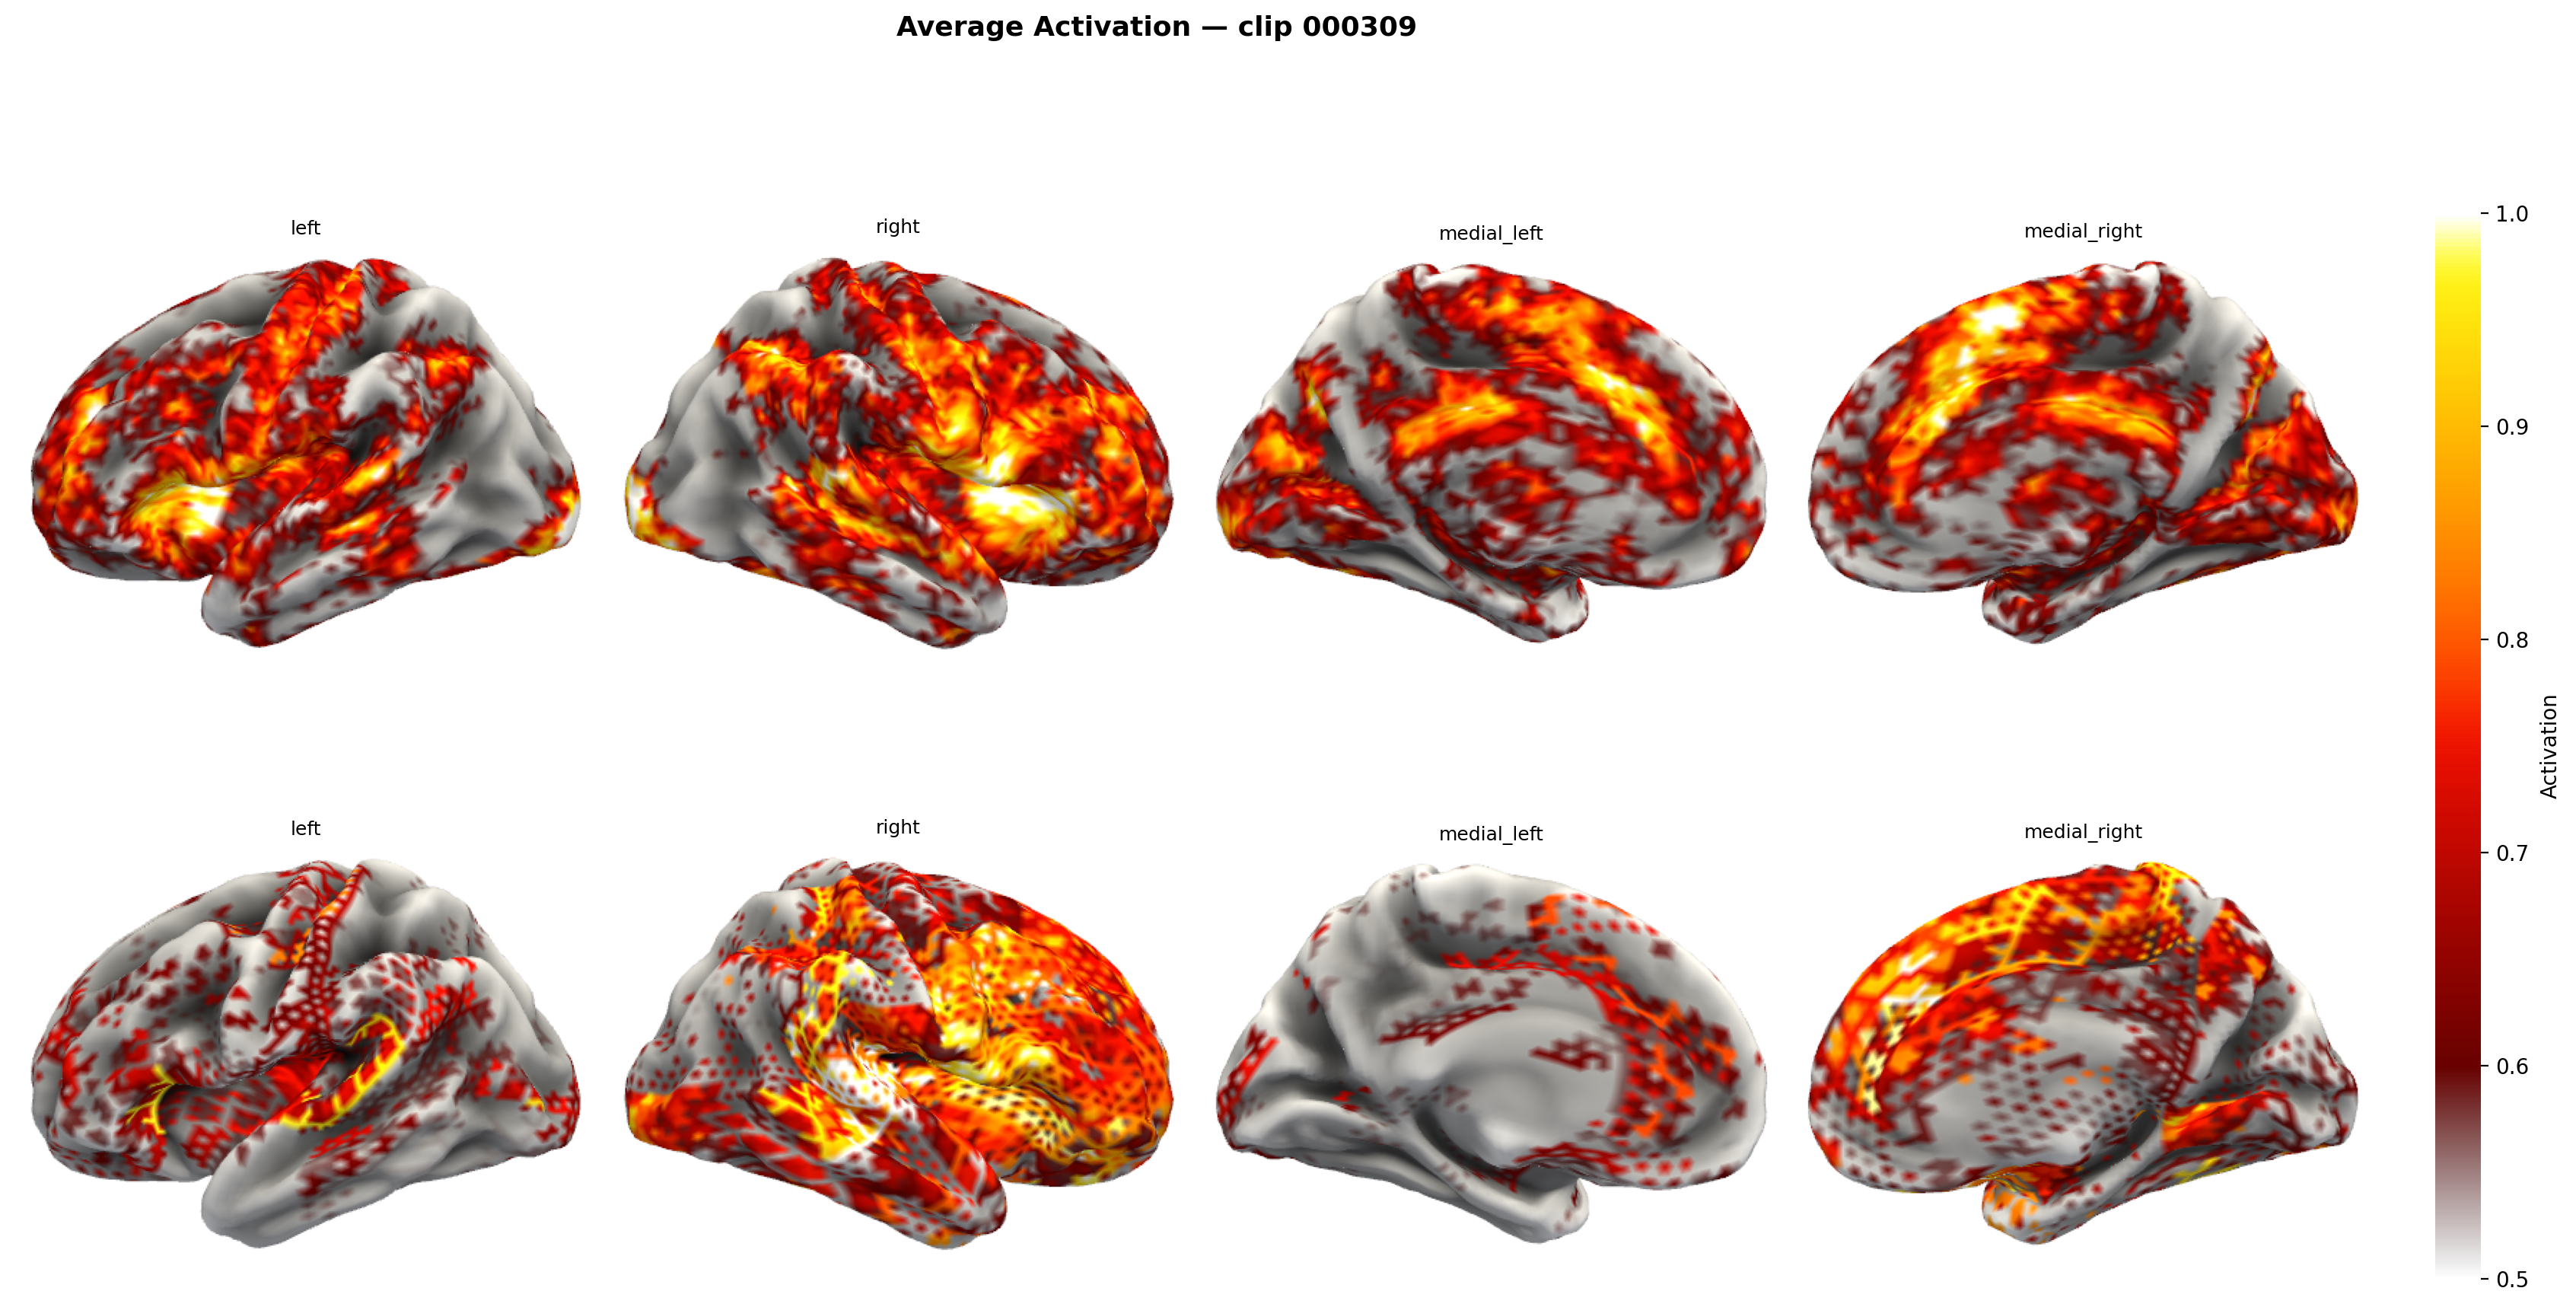
\includegraphics[width=\textwidth]{plots/brain_viz_000309_activation_map.png}
\caption{Клип 000309}\label{fig:clip309}
\end{subfigure}\hfill
\begin{subfigure}[b]{0.32\textwidth}
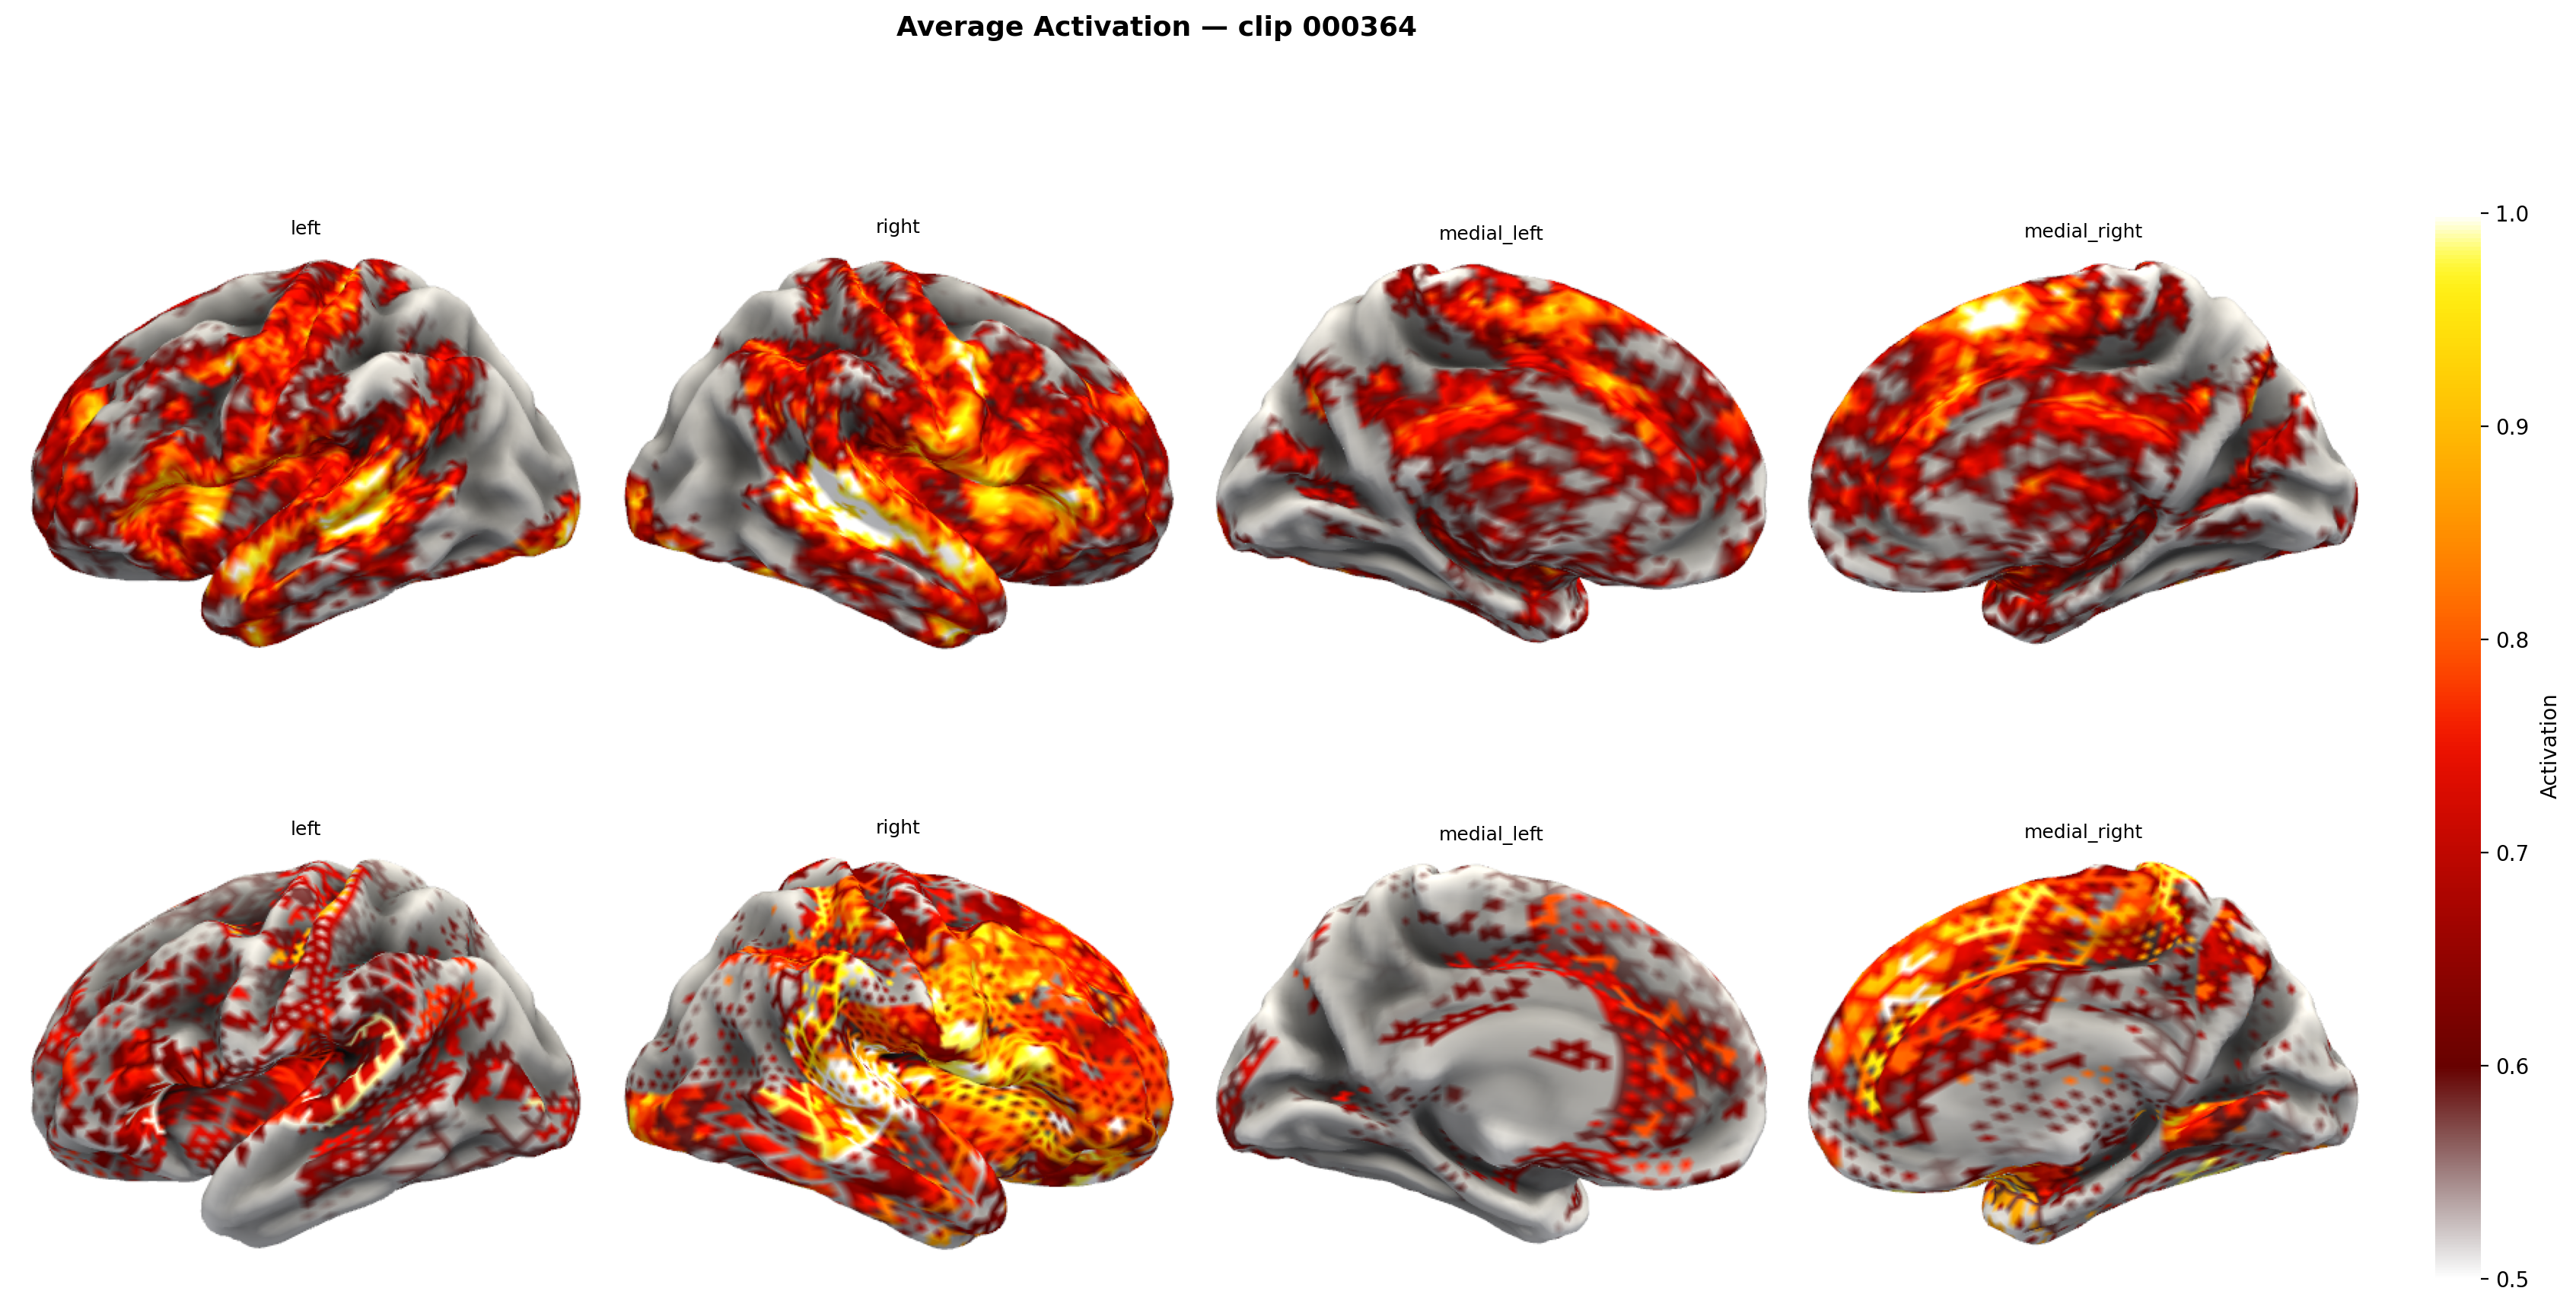
\includegraphics[width=\textwidth]{plots/brain_viz_000364_activation_map.png}
\caption{Клип 000364}\label{fig:clip364}
\end{subfigure}\hfill
\begin{subfigure}[b]{0.32\textwidth}
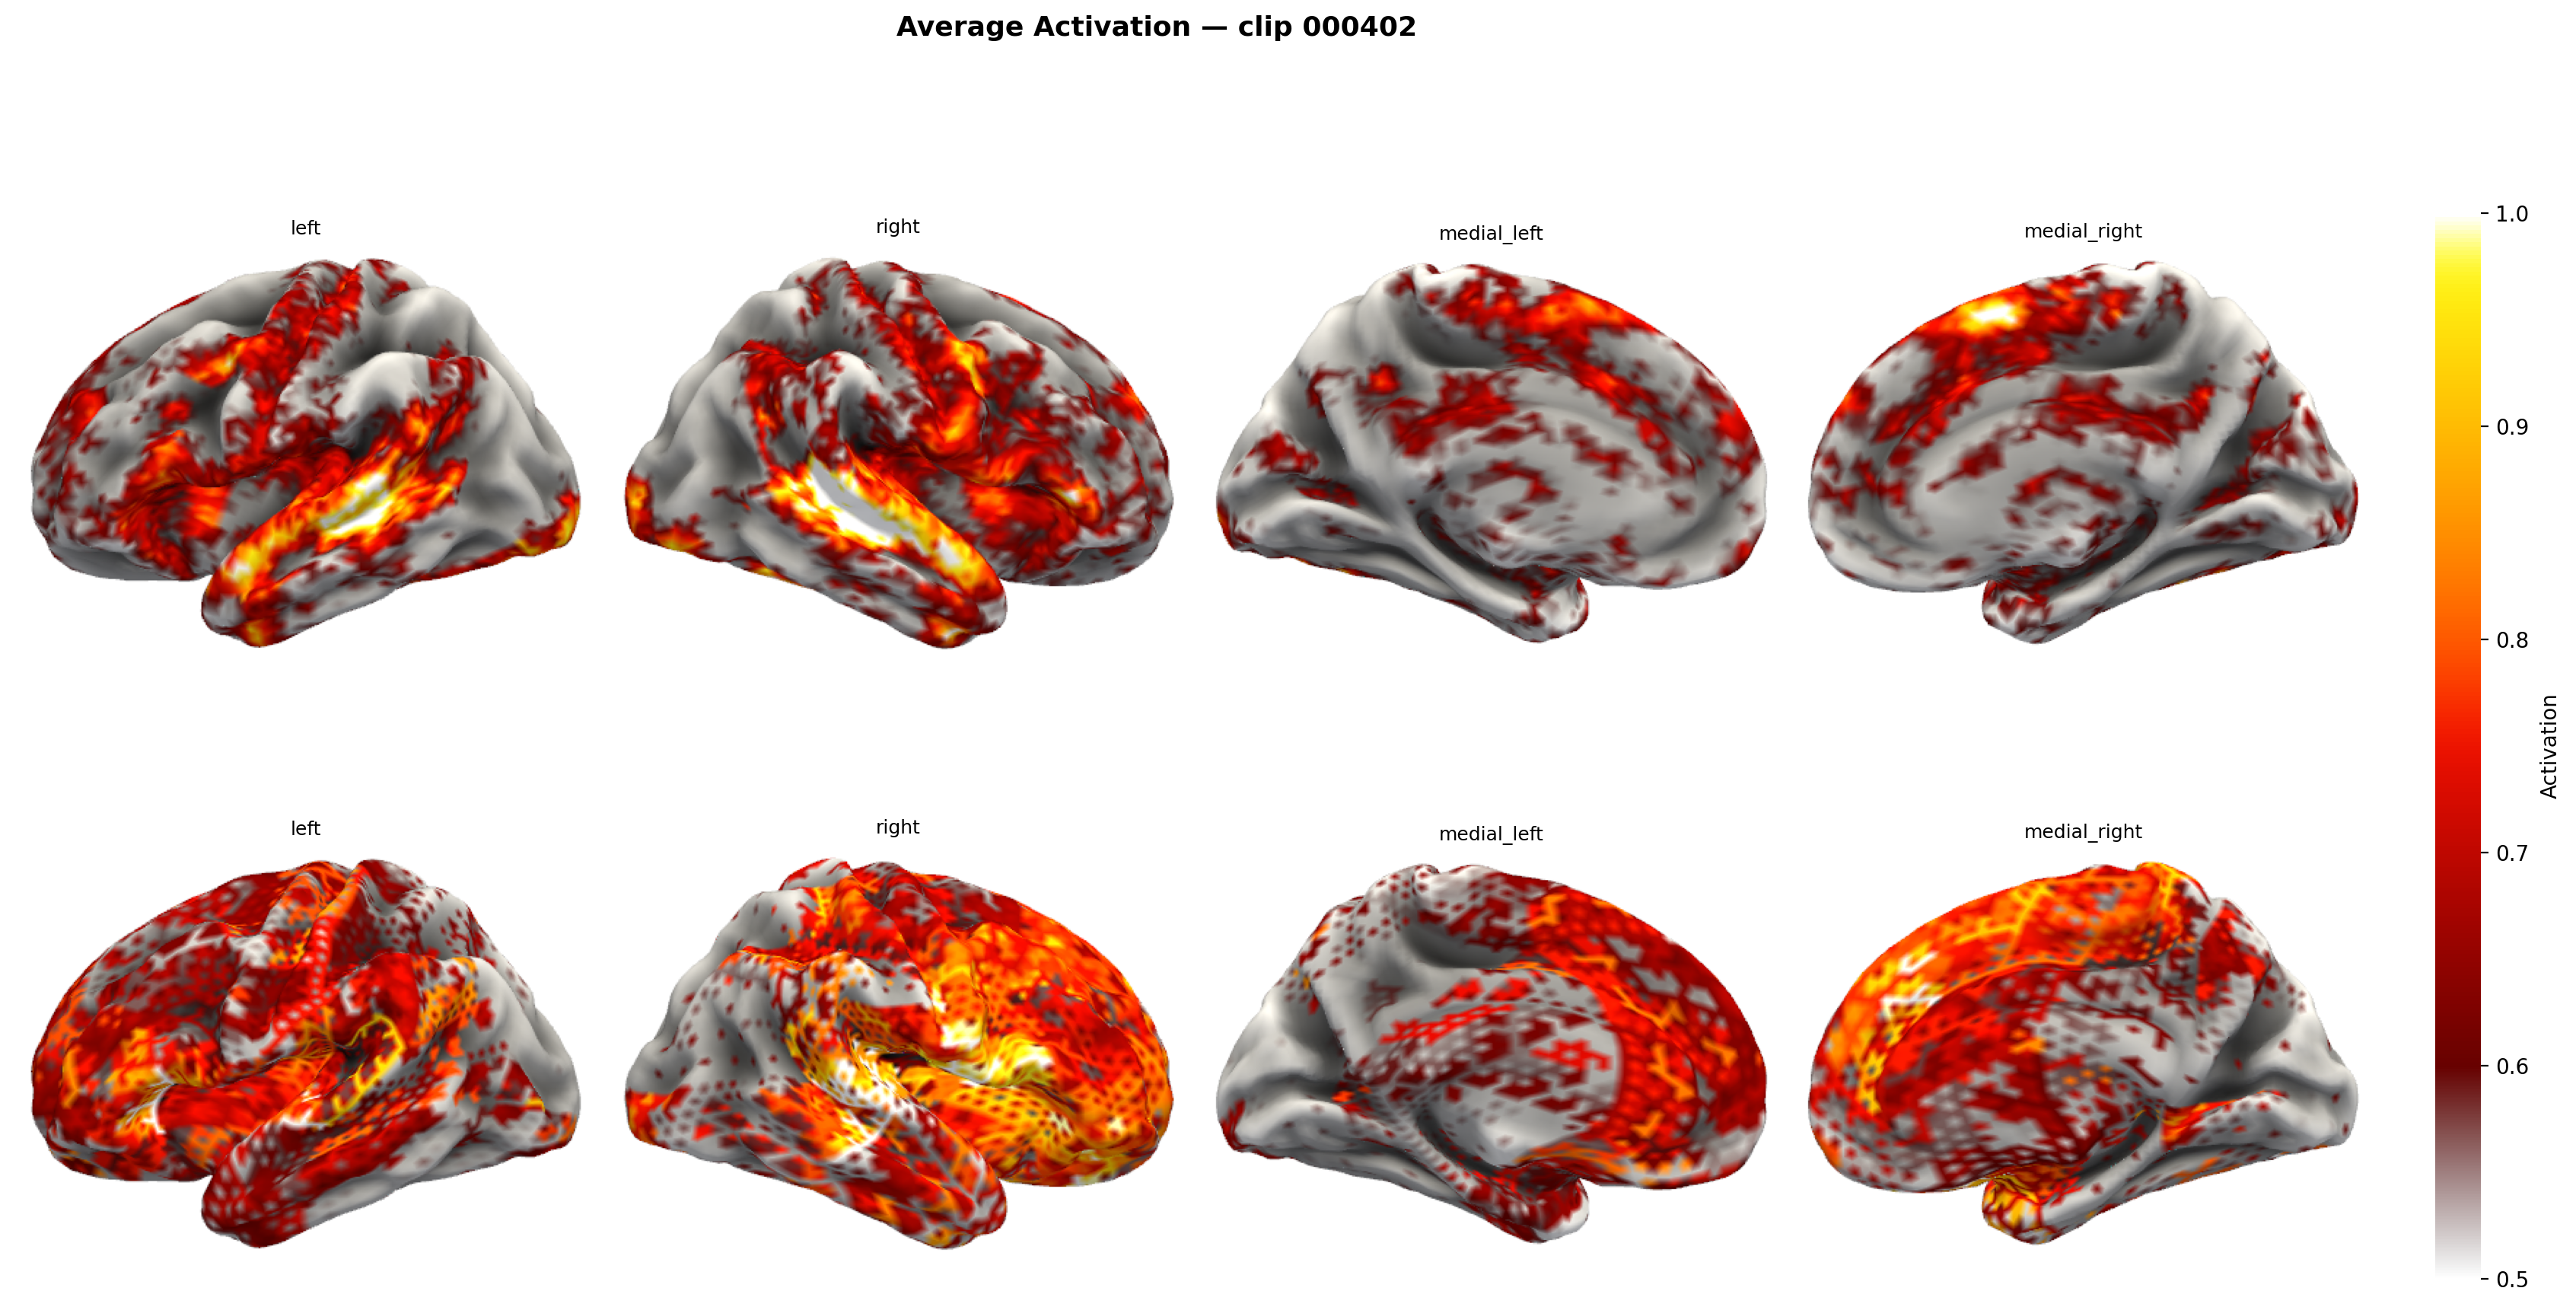
\includegraphics[width=\textwidth]{plots/brain_viz_000402_activation_map.png}
\caption{Клип 000402}\label{fig:clip402}
\end{subfigure}
\caption{Предсказанные карты кортикальной активности для шести
отложенных клипов набора CINE Brain. Для каждого клипа показаны
латеральный и медиальный виды обоих полушарий при двух порогах
отображения (\texttt{plots/brain\_viz\_*\_activation\_map.png}).}
\label{fig:clips}
\end{figure}

% ============================================================================
\section{Обсуждение}
\label{sec:discussion}

\subsection{Интерпретация полученного результата}
\label{sec:disc-interpretation}

Полученное значение $r = 0{,}7278$ следует интерпретировать строго:
это согласие облегчённой модели с \emph{эталонными предсказаниями}
на отложенных клипах (задача воспроизведения поведения фоновой
модели на новых данных), а не прямая корреляция с измеренным
фМРТ-сигналом. В такой постановке результат показывает, что стек
синтеза из $9{,}7$~млн обучаемых параметров способен почти полностью
воспроизвести функциональное отображение эталона, сохраняя при
этом возможность обучения на одной GPU и edge-развёртывания (в
проекте предусмотрены ONNX-экспорт с INT8-квантованием и
браузерный рантайм). Деградация валидационной метрики после
эпохи~$52$ при растущей обучающей кривой указывает на то, что
узким местом является не ёмкость модели, а объём и разнообразие
учебного корпуса ($160$~обучающих клипов); это согласуется
с наблюдениями литературы о роли масштаба данных в мультисубъектных
энкодерах~\cite{Scotti2024}.

Архитектурные решения имеют независимую научную мотивацию:
HRF-смещение внимания и обучаемая гемодинамическая свёртка переносят
известную нейрофизиологию~\cite{Glover1999,Lindquist2019} в
индуктивный bias, а FiLM-кондиционирование открывает путь к дешёвой
адаптации модели к новым субъектам~\cite{Perez2018}.

\subsection{Биоинженерный и нейронаучный импакт}
\label{sec:disc-impact}

Для биоинженерии и нейронауки Flora предлагает три конкретных
направления, в которых компактная модель мозга может оказаться
полезной уже сейчас:

\begin{itemize}[leftmargin=*]
    \item \textbf{Реабилитационные интерфейсы мозг--компьютер (BCI).}
          При добавлении субъектно-зависимой FiLM-надстройки Flora
          может служить основой для адаптивного декодера, который
          быстро <<подстраивается>> под нового пациента без
          переобучения всей сети.
    \item \textbf{Скрининг когнитивных нарушений.}
          Отклонения между предсказанными и измеренными ответами
          коры~--- прямой количественный показатель
          <<нейрофизиологического несоответствия>>, применимый для
          раннего выявления деменции, расстройств аутистического
          спектра и др.
    \item \textbf{Дополненная нейрохирургическая навигация.}
          Прогноз кортикального отклика на стимулы и предсказание
          областей активации помогают планировать операции в
          функционально значимых зонах.
\end{itemize}

Эти направления согласуются с приоритетами научных фондов,
поддерживающих мультидисциплинарные проекты на стыке инженерии
и нейронаук: NSF, NIH (BRAIN Initiative), ERC, Horizon Europe,
РФФИ/РНФ. Открытый исходный код и воспроизводимые чекпоинты
делают Flora удобной заявкой для совместных грантов с медицинскими
и инженерными группами.

\subsection{Сравнение с фоном нейро-ИИ}
\label{sec:disc-comparison}

Современный фронт нейро-ИИ связан с крупными
тримодальными моделями~\cite{dAscoli2026tribe,dAscoli2026tribev2},
обучаемыми на сотнях часов записей и сотнях субъектов. Flora
\emph{не} конкурирует с ними напрямую по охвату данных и числу
субъектов; её ценность~--- в иной точке проектного пространства:
\emph{компактность, воспроизводимость, развёртываемость}. В тех
случаях, когда воспроизведение эксперимента с нуля должно быть
доступно ограниченной лаборатории (например, в региональных
исследовательских центрах или в клиниках), компактная модель
оказывается критически важной.

\subsection{Потенциальные социальные эффекты}
\label{sec:disc-social}

Как и любые модели мозга, Flora несёт социальные риски (интерпретация
индивидуальных данных, защита приватности, использование для
манипулятивных интерфейсов). Мы явно ограничиваем область применения
настоящей работы клинически и исследовательски мотивированными
задачами, для которых получено информированное согласие участников
в соответствии с Хельсинкской декларацией и местными этическими
регламентами (см. этические замечания в~\cref{app:ethics}).

% ============================================================================
\section{Ограничения}
\label{sec:limitations}

\begin{enumerate}[label=(\arabic*), leftmargin=*]
    \item Основная метрика~--- согласие с предсказаниями эталона,
          а не с сырым фМРТ; файнтюнинг на реальном сигнале
          (Phase~$3$) реализован, но его результаты не зафиксированы.
    \item Отображение fsaverage5 $\rightarrow$ Schaefer-400
          выполнено чанковым усреднением (placeholder в коде),
          а не точным атласным соответствием.
    \item Динамика обучения восстановлена схематично; поэпохальный
          лог отсутствует.
    \item Один субъект в обучающем корпусе ($n\_subjects = 1$);
          ЭЭГ-канал CineBrain не используется.
    \item Грубая временная дискретизация клипа ($T = 5$ шагов)
          и расхождение принятого TR~$=1{,}5$~с с исходным
          TR~$=0{,}8$~с CineBrain~\cite{Gao2025cinebrain}
          требуют уточнения.
    \item Отсутствуют тесты статистической значимости и шумовой
          потолок.
    \item Число обучающих клипов ($160$) ограничено; расширение
          на большее разнообразие аудиовизуального контента~---
          естественное направление развития.
\end{enumerate}

% ============================================================================
\section{Заключение}
\label{sec:conclusion}

Представлена Flora~--- лёгкая мультимодальная модель кодирования
коры, сочетающая замороженные компактные энкодеры ($67{,}3$~млн
параметров) с обучаемым MoE-трансформером синтеза
($9{,}7$--$14$~млн параметров), нейрофизическими априорными
ограничениями (HRF-свёртка, HRF-смещение внимания) и экономичным
FiLM-механизмом персубъектной адаптации. На учебном корпусе
из $200$~клипов CINE Brain модель достигает $r = 0{,}7278$ на
$40$~отложенных клипах (лучшая эпоха $52$).

Прямые направления развития:
(i)~файнтюнинг на реальном фМРТ-сигнале;
(ii)~точное атласное отображение fsaverage5 $\rightarrow$
Schaefer-400;
(iii)~систематические абляции (HRF, MoE, гейтинг, FiLM);
(iv)~оценка статистической значимости и шумового потолка;
(v)~расширение корпуса за счёт других открытых наборов;
(vi)~прямое клиническое пилотирование на пациентах с
нейродегенеративными заболеваниями.

% ============================================================================
\section*{Благодарности}
\addcontentsline{toc}{section}{Благодарности}

Авторы выражают благодарность авторам открытого набора CINE
Brain~\cite{CINEBrain,Gao2025cinebrain} за предоставленные
данные, разработчикам PyTorch Lightning и сообществу
FreeSurfer/nilearn за воспроизводимый инструментарий.

% ============================================================================
\bibliographystyle{plain}
\bibliography{references}

% ============================================================================
\newpage
\appendix

\section{Полные гиперпараметры}
\label{app:hyper}

\begin{table}[H]
\centering
\caption{Архитектурные гиперпараметры: чекпоинт POC (фактические
из \texttt{hyper\_parameters}) и полная конфигурация по умолчанию
(\texttt{flora/v3\_model.py}).}
\label{tab:app-model}
\small
\begin{tabular}{lcc}
\toprule
Параметр & POC (чекпоинт) & Полная (default) \\
\midrule
hidden\_dim        & 256 & 512 \\
num\_layers        & 2   & 4 \\
num\_heads         & 4   & 8 \\
num\_experts       & 4   & 8 \\
top\_k             & 2   & 2 \\
ff\_mult           & 2   & 2 \\
proj. intermediate & 768 & 768 \\
dropout            & 0{,}3 & 0{,}1 \\
modality dropout   & 0{,}5 & 0{,}3 \\
stochastic depth max & --- & 0{,}2 \\
HRF: TR / ядро     & 1{,}5~с / 8~TR & 1{,}5~с / 8~TR \\
n\_vertices        & 400 & 400 (поддерживается 20\,484) \\
n\_subjects        & 1   & 3 (до 25) \\
max\_seq\_len      & 1024--2048 & 2048 \\
\bottomrule
\end{tabular}
\end{table}

\begin{table}[H]
\centering
\caption{Гиперпараметры обучения: основной эксперимент
(\texttt{train\_lightning.py} + чекпоинт) и фазы расширенного
пайплайна (\texttt{v3\_train.py}).}
\label{tab:app-train}
\small
\begin{tabular}{lccc}
\toprule
Параметр & Основной & Phase 2 & Phase 3 \\
\midrule
lr                  & $10^{-3}$ & $3\cdot10^{-4}$ & $5\cdot10^{-5}$ \\
backbone lr         & --- & --- & $5\cdot10^{-6}$ \\
weight decay        & 0{,}1 & $10^{-2}$ & $10^{-2}$ \\
эпохи (max)         & 100 & 60 & 30 \\
батч                & 16 & 8 & 8 \\
прогрев (эпохи)     & 3 & 3 & 2 \\
клиппинг            & 1{,}0 & 1{,}0 & 0{,}5 \\
modality dropout    & 0{,}5 & 0{,}3 & 0{,}1 \\
веса потерь         & \eqref{eq:kdtotal} & $0{,}6/0{,}2/0{,}1/0{,}05/0{,}01$ & \eqref{eq:fmriloss} \\
AMP                 & опционально & да & да \\
seed                & 42 & --- & --- \\
\bottomrule
\end{tabular}
\end{table}

\section{Дополнительные фигуры}
\label{app:figures}

\begin{figure}[H]
\centering
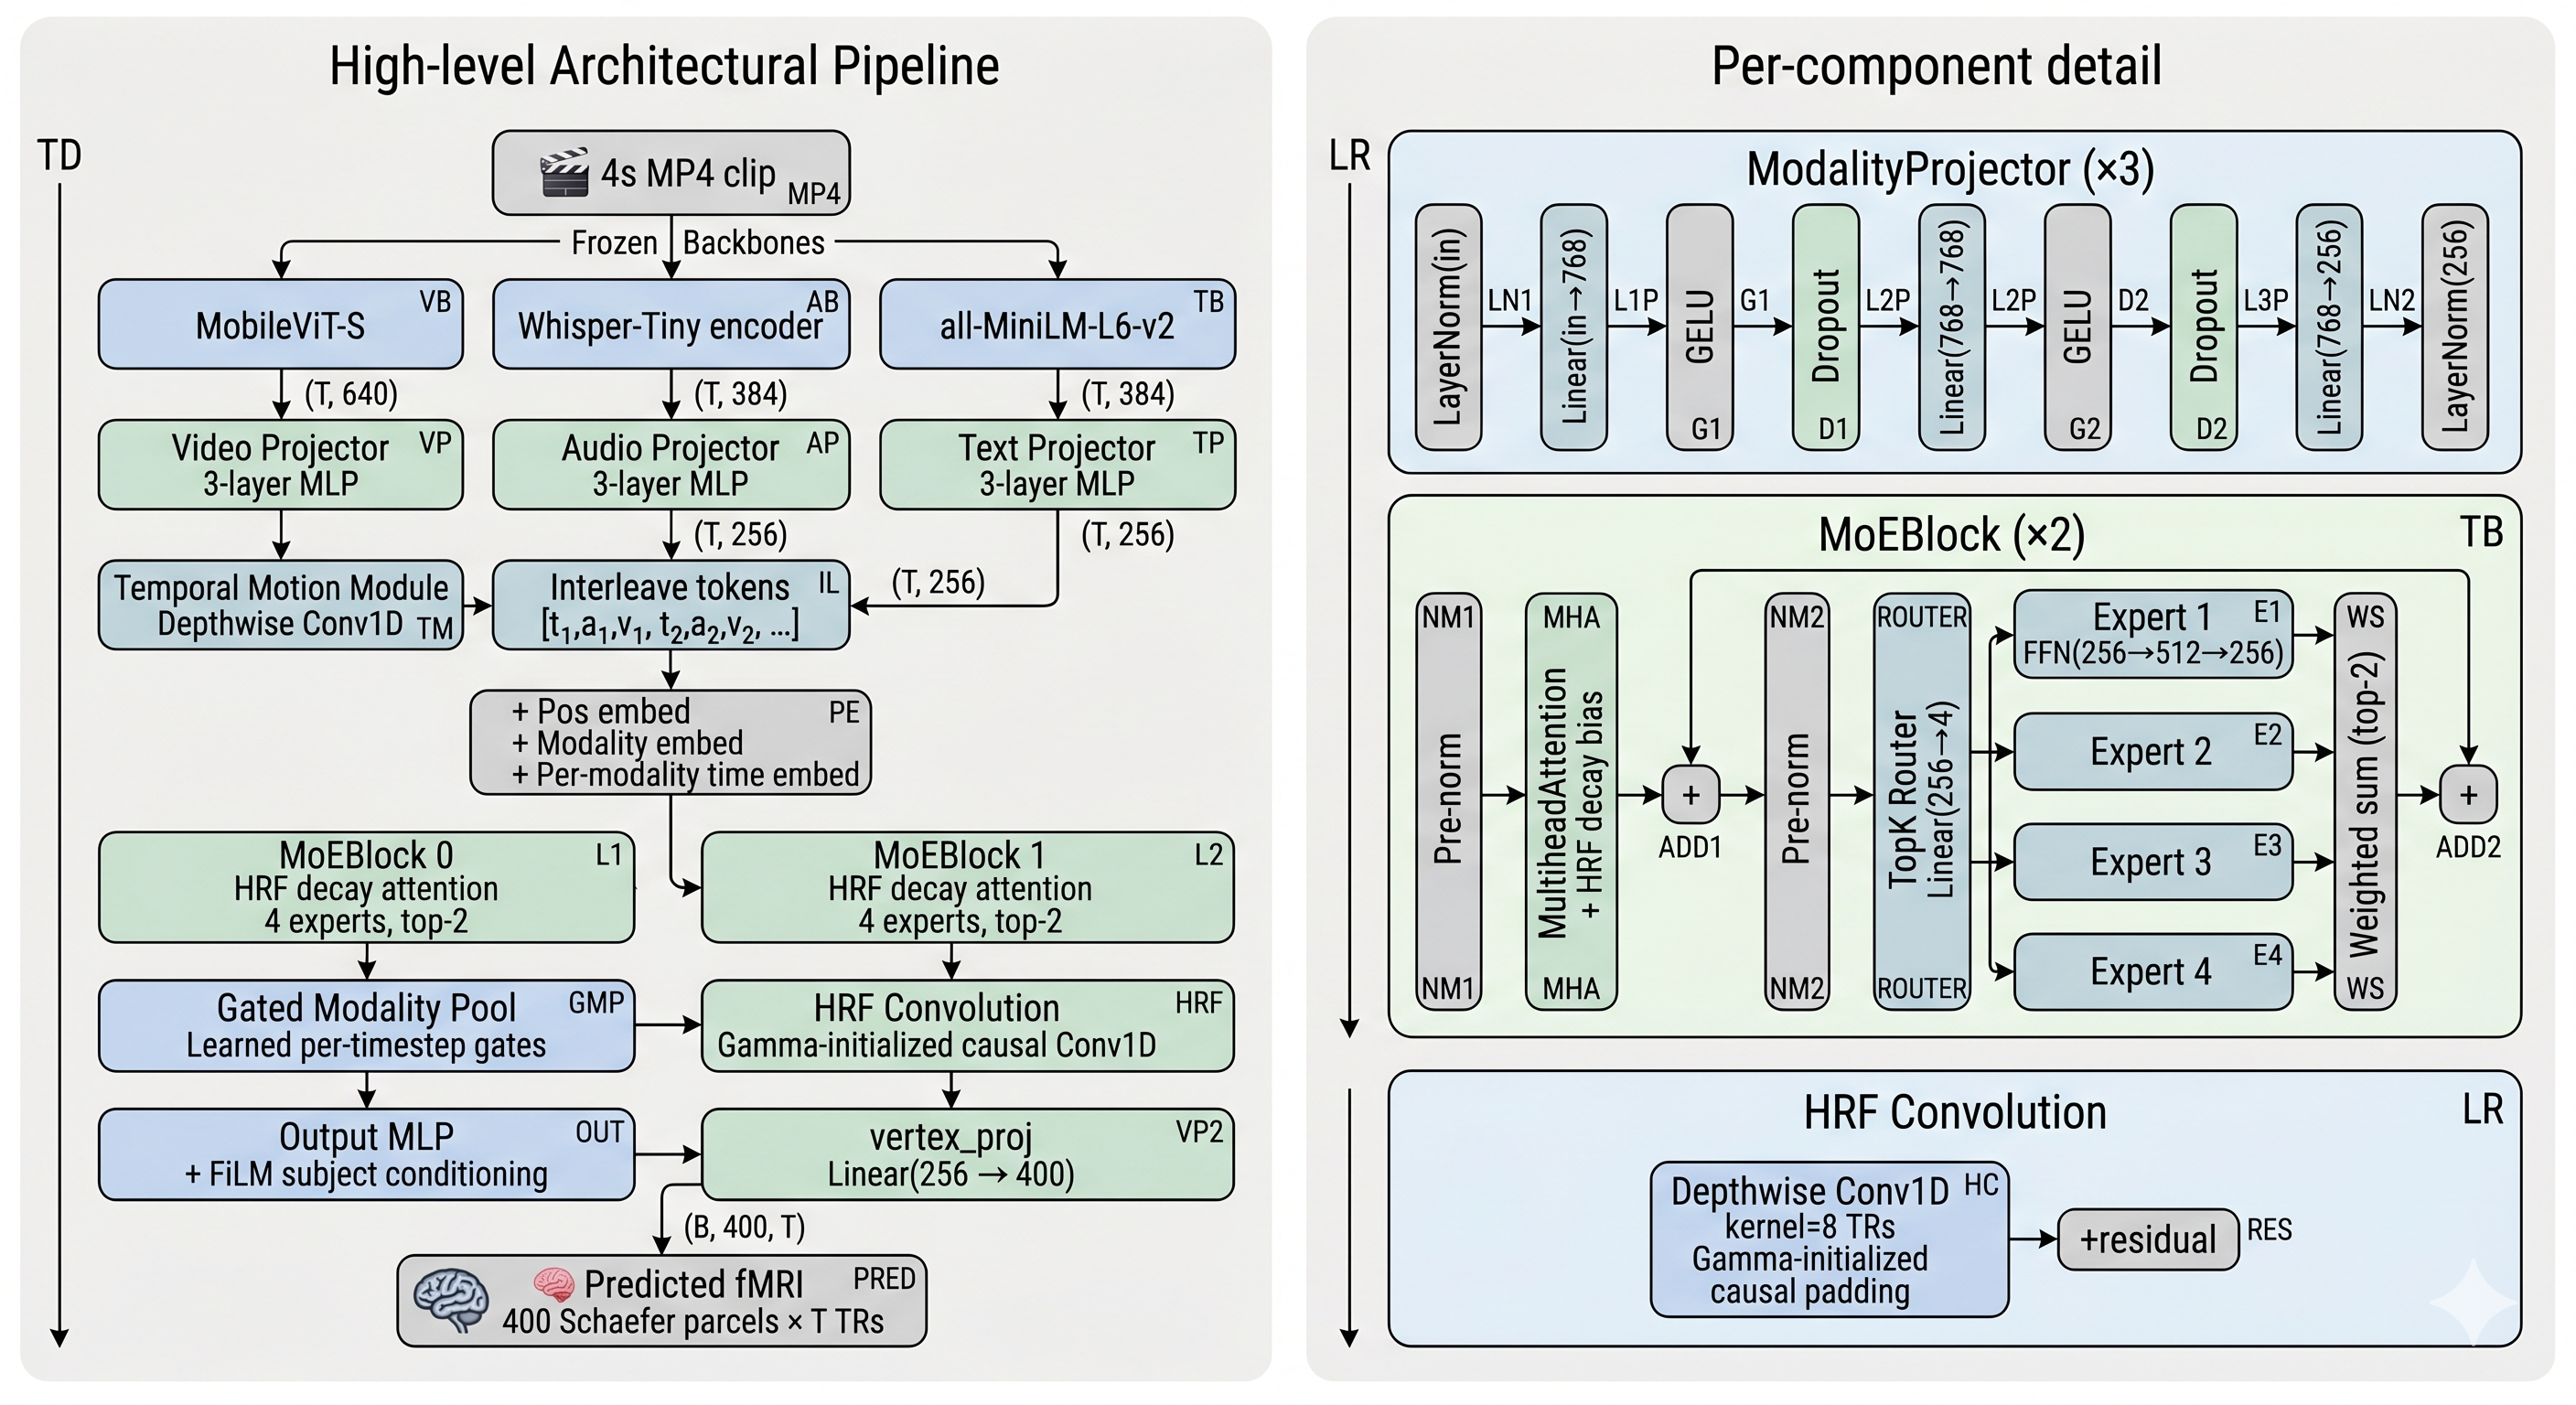
\includegraphics[width=0.9\textwidth]{assets/flora_v3_architecture.png}
\caption{Детальная диаграмма архитектуры Flora~v3 (генерируется
\texttt{flora/architecture\_diagram.py};
\texttt{assets/flora\_v3\_architecture.png}).}
\label{fig:v3arch}
\end{figure}

\begin{figure}[H]
\centering
\begin{subfigure}[b]{0.49\textwidth}
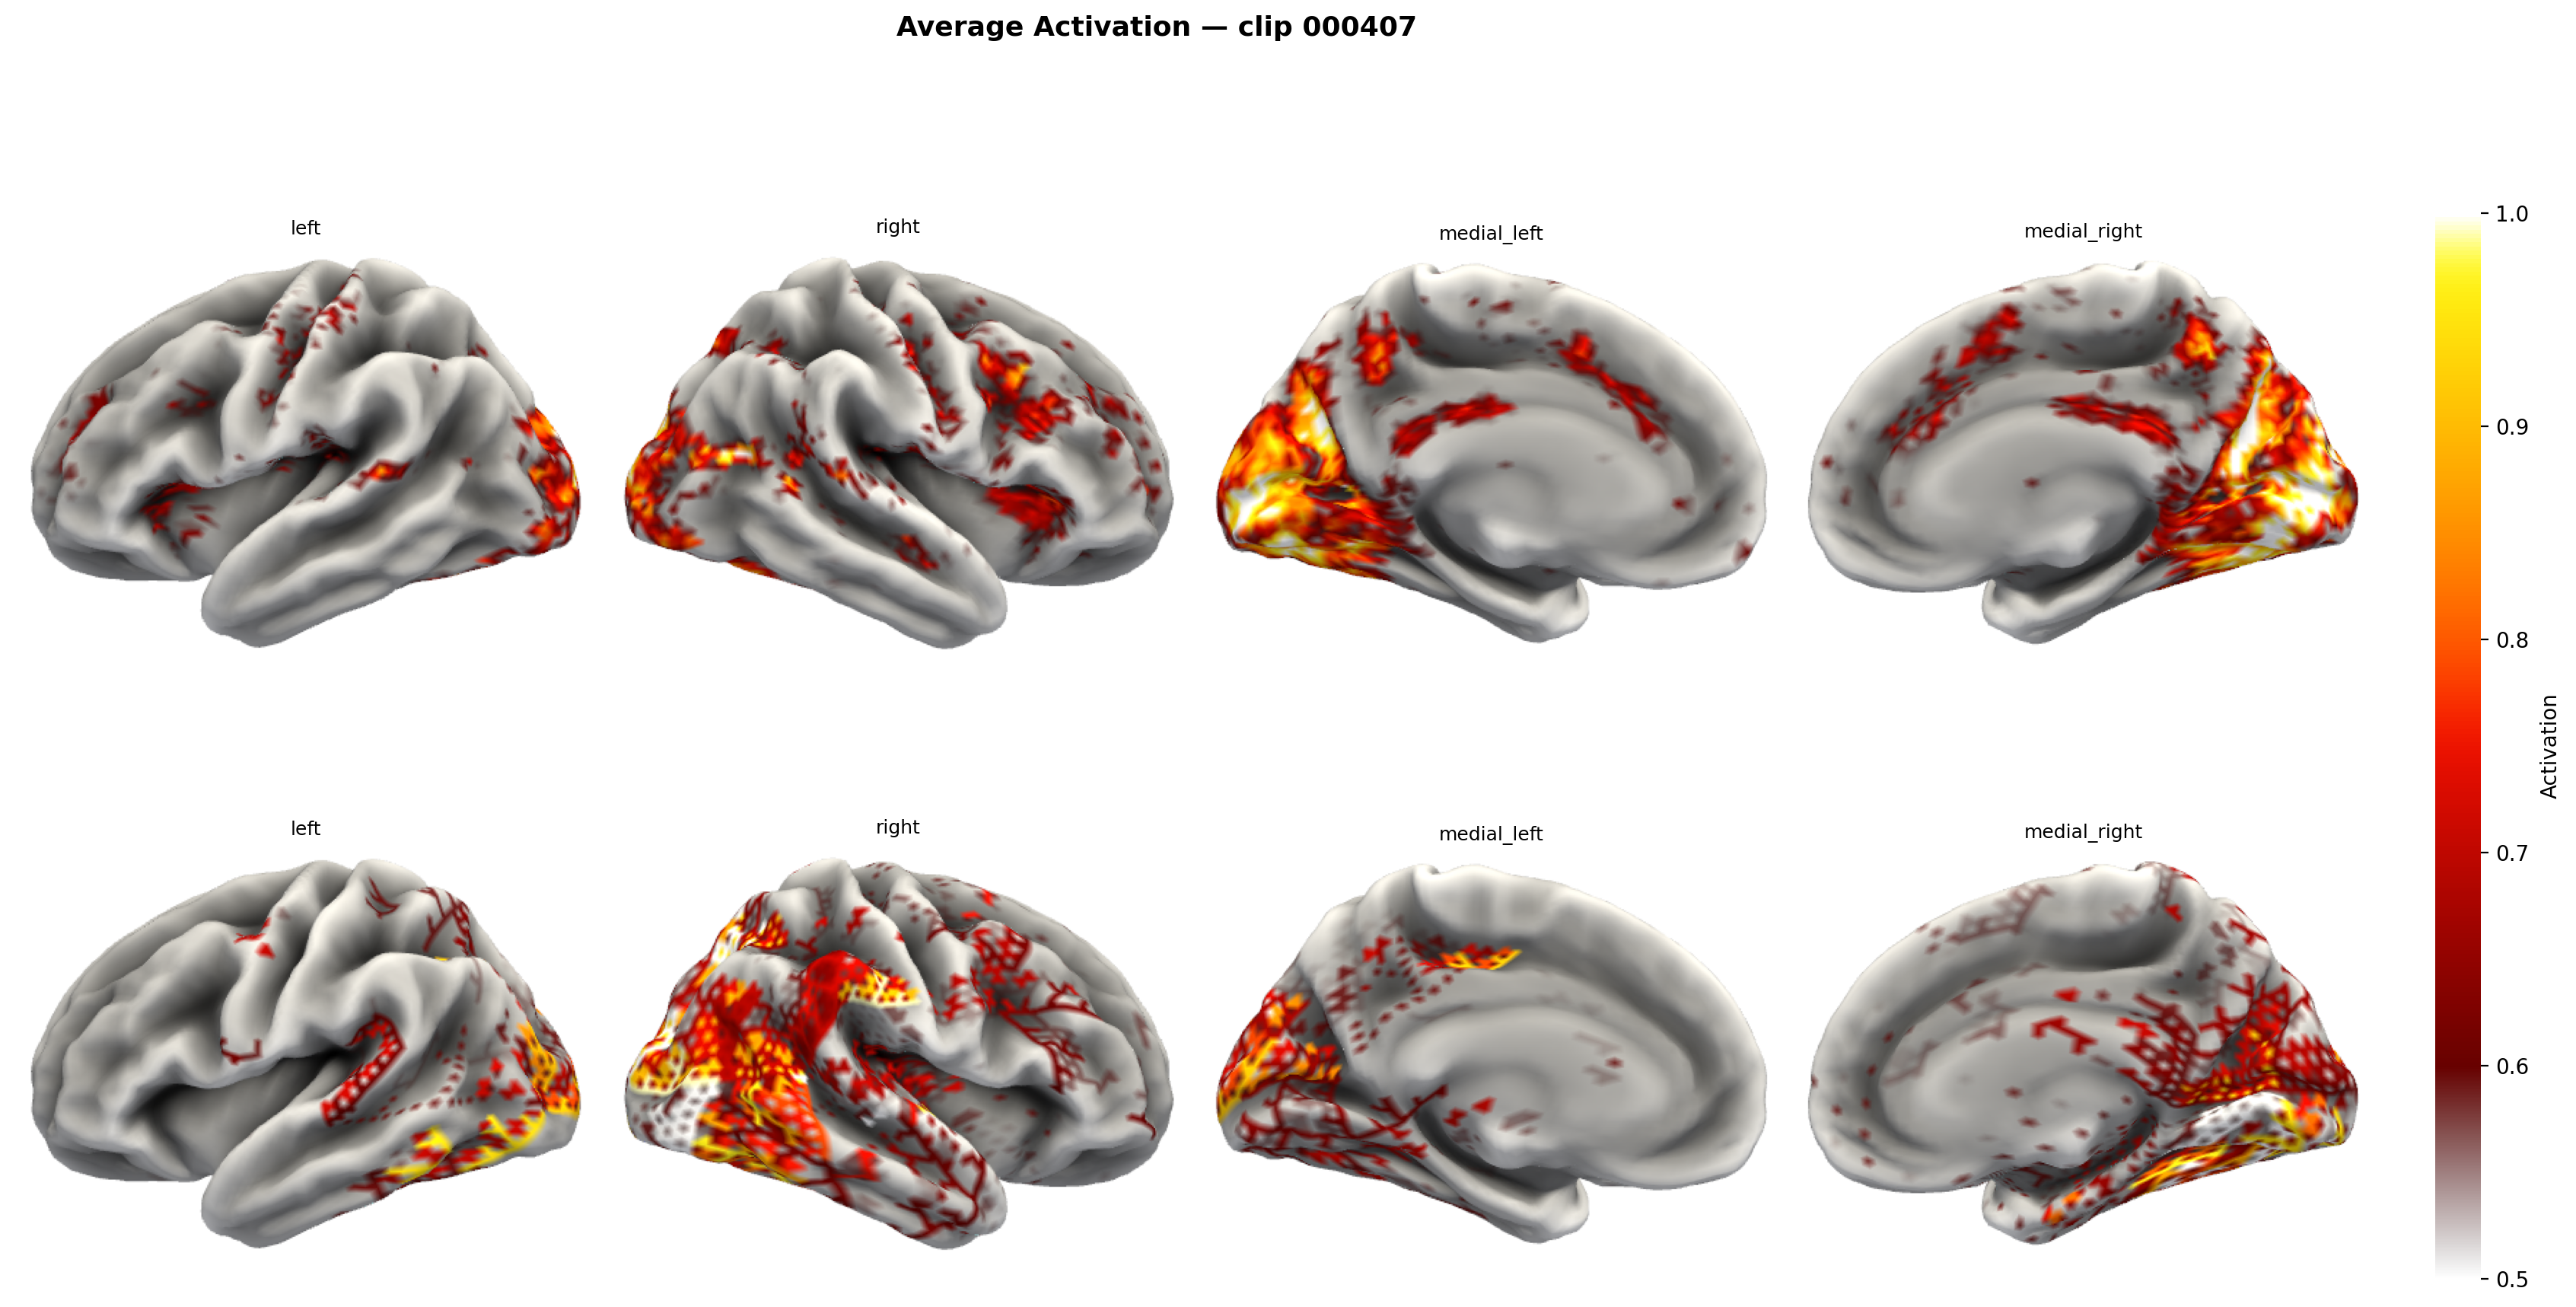
\includegraphics[width=\textwidth]{plots/brain_viz_000407_activation_map.png}
\caption{Клип 000407}
\end{subfigure}\hfill
\begin{subfigure}[b]{0.49\textwidth}
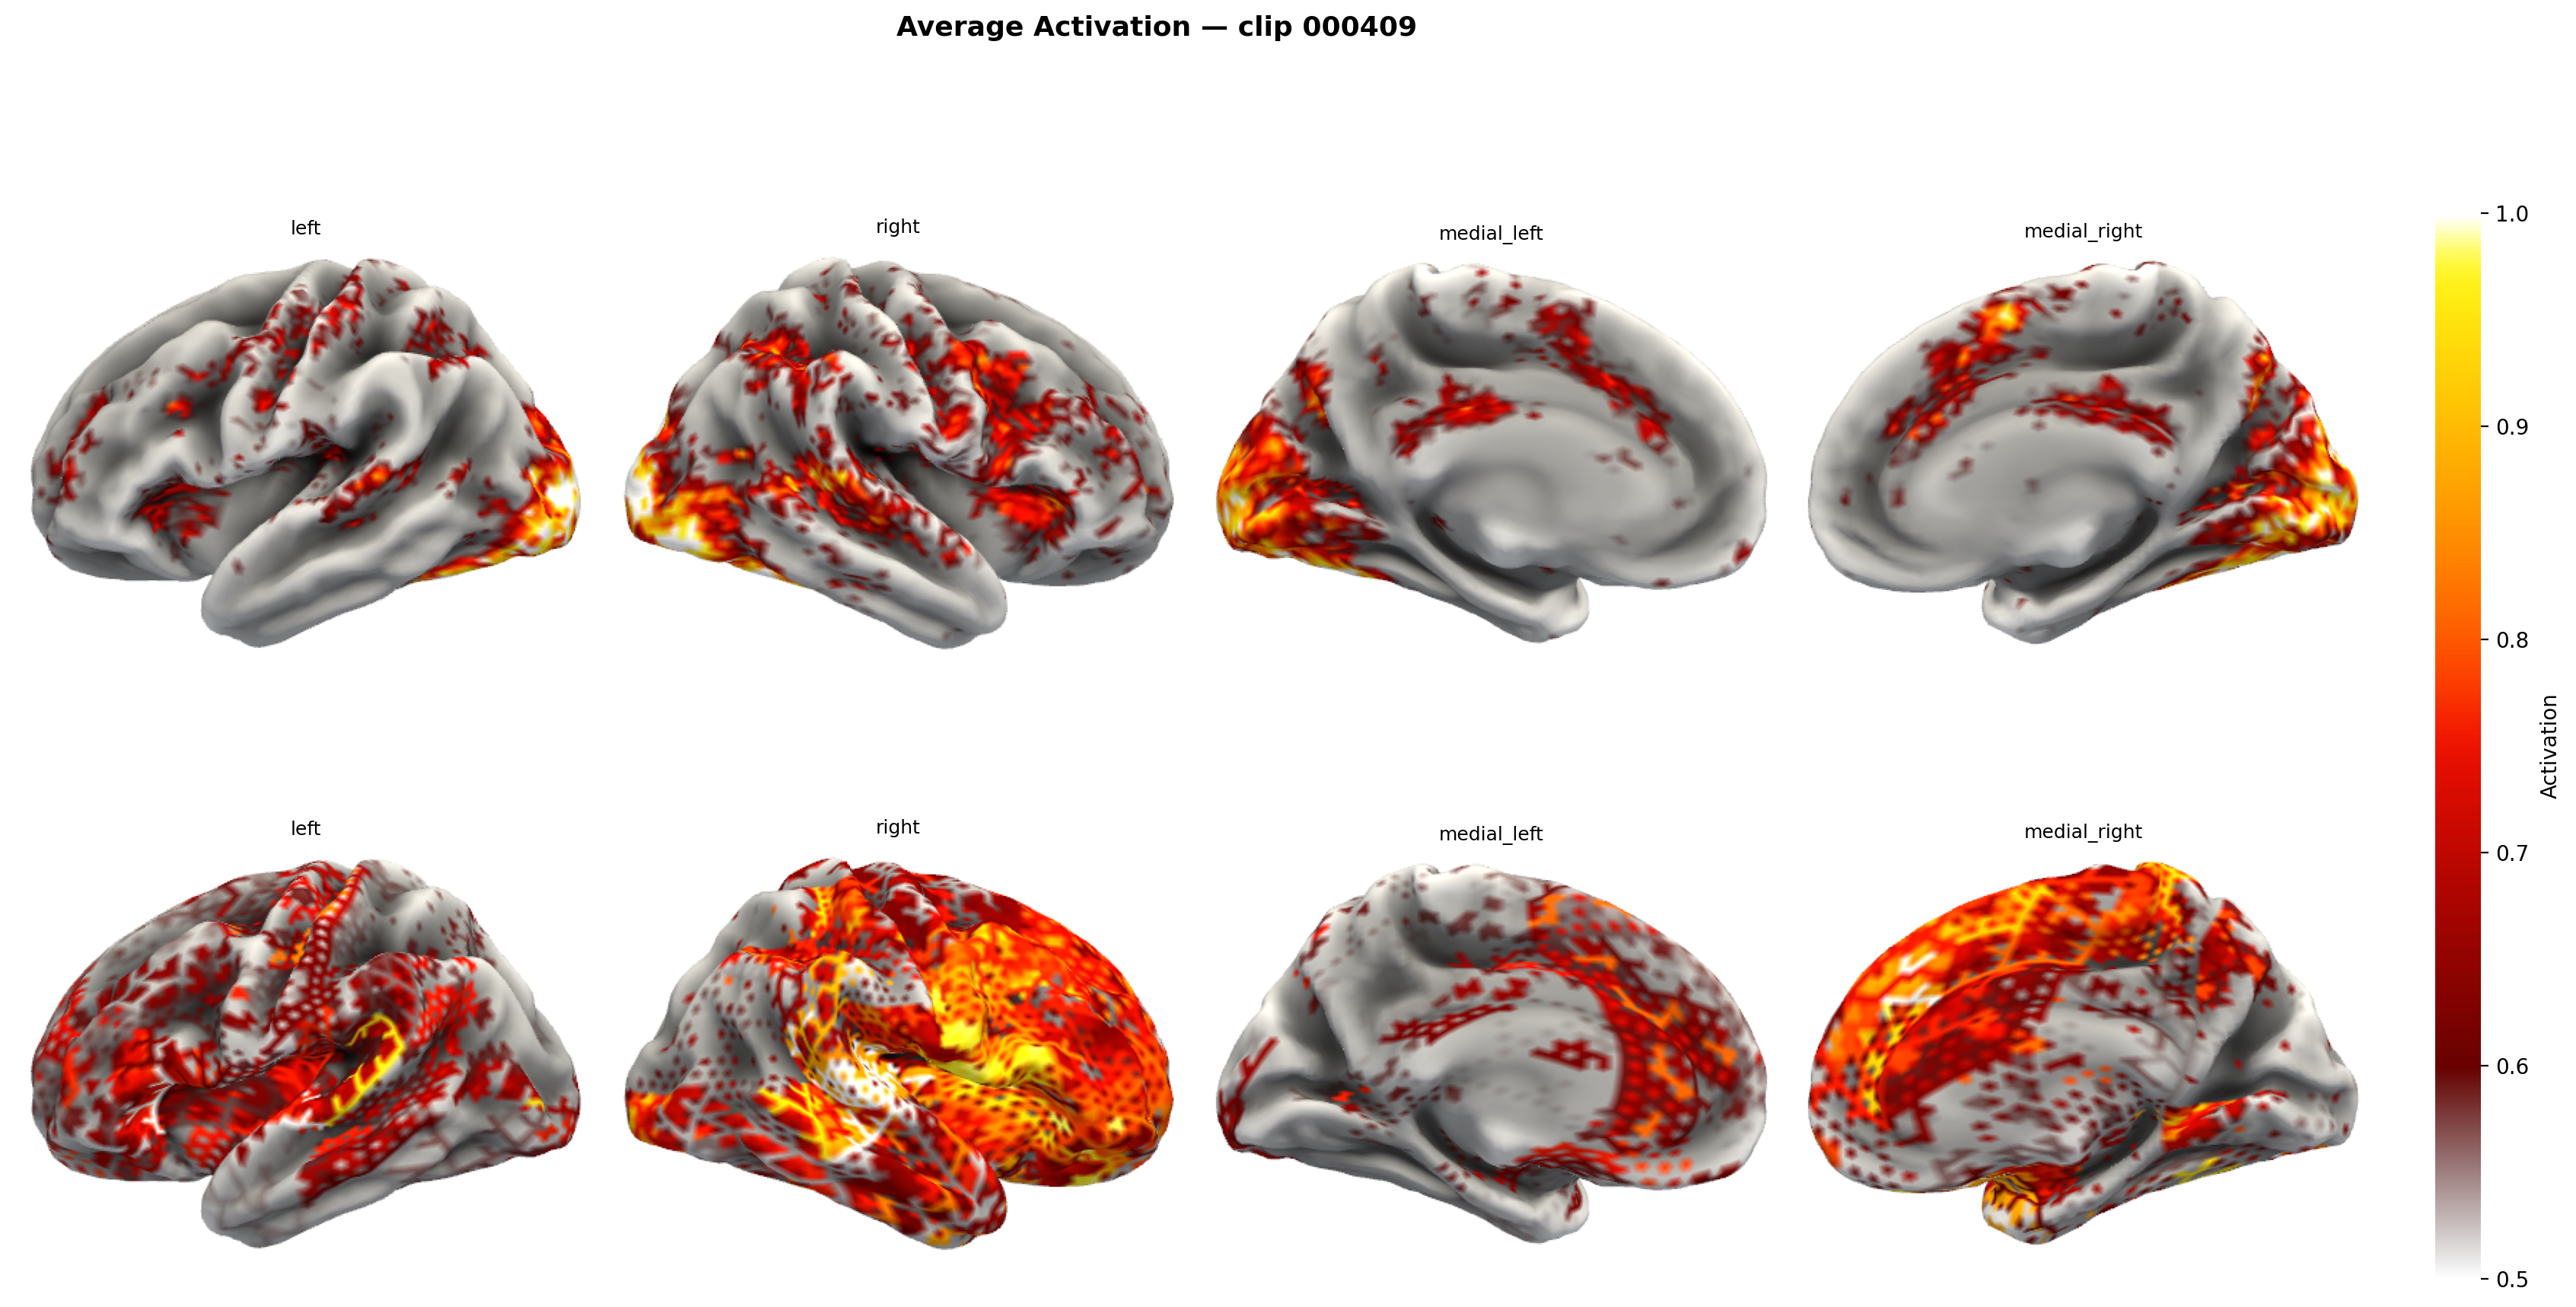
\includegraphics[width=\textwidth]{plots/brain_viz_000409_activation_map.png}
\caption{Клип 000409}
\end{subfigure}

\medskip
\begin{subfigure}[b]{0.49\textwidth}
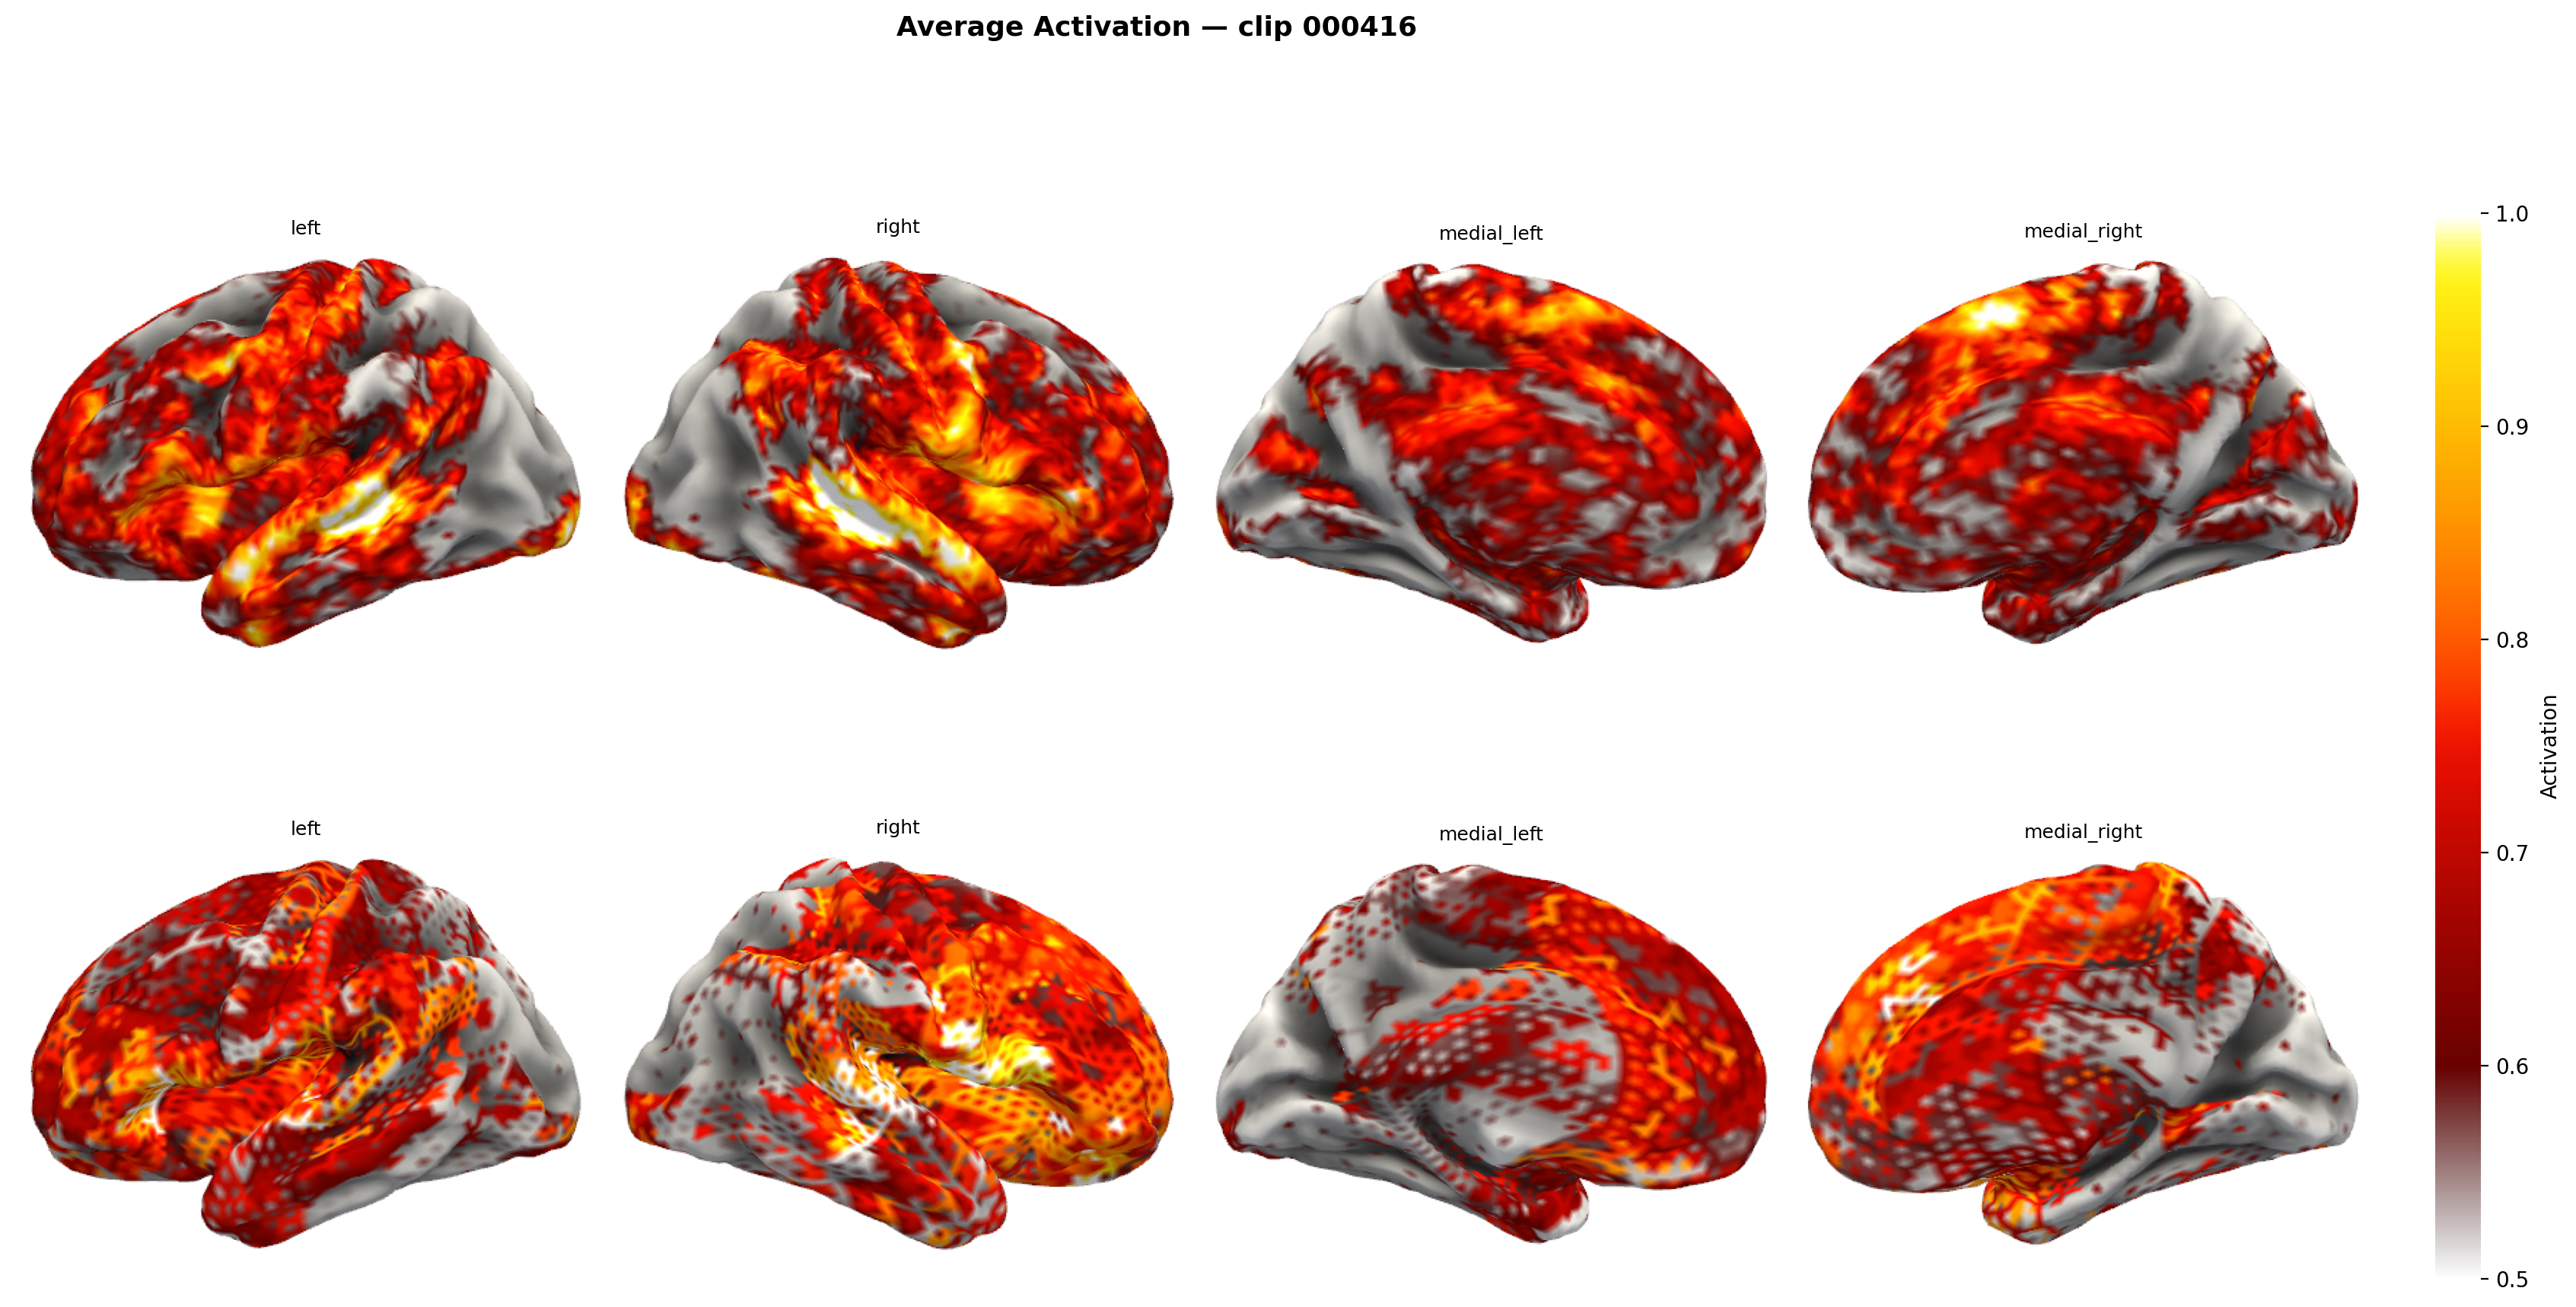
\includegraphics[width=\textwidth]{plots/brain_viz_000416_activation_map.png}
\caption{Клип 000416}
\end{subfigure}\hfill
\begin{subfigure}[b]{0.49\textwidth}
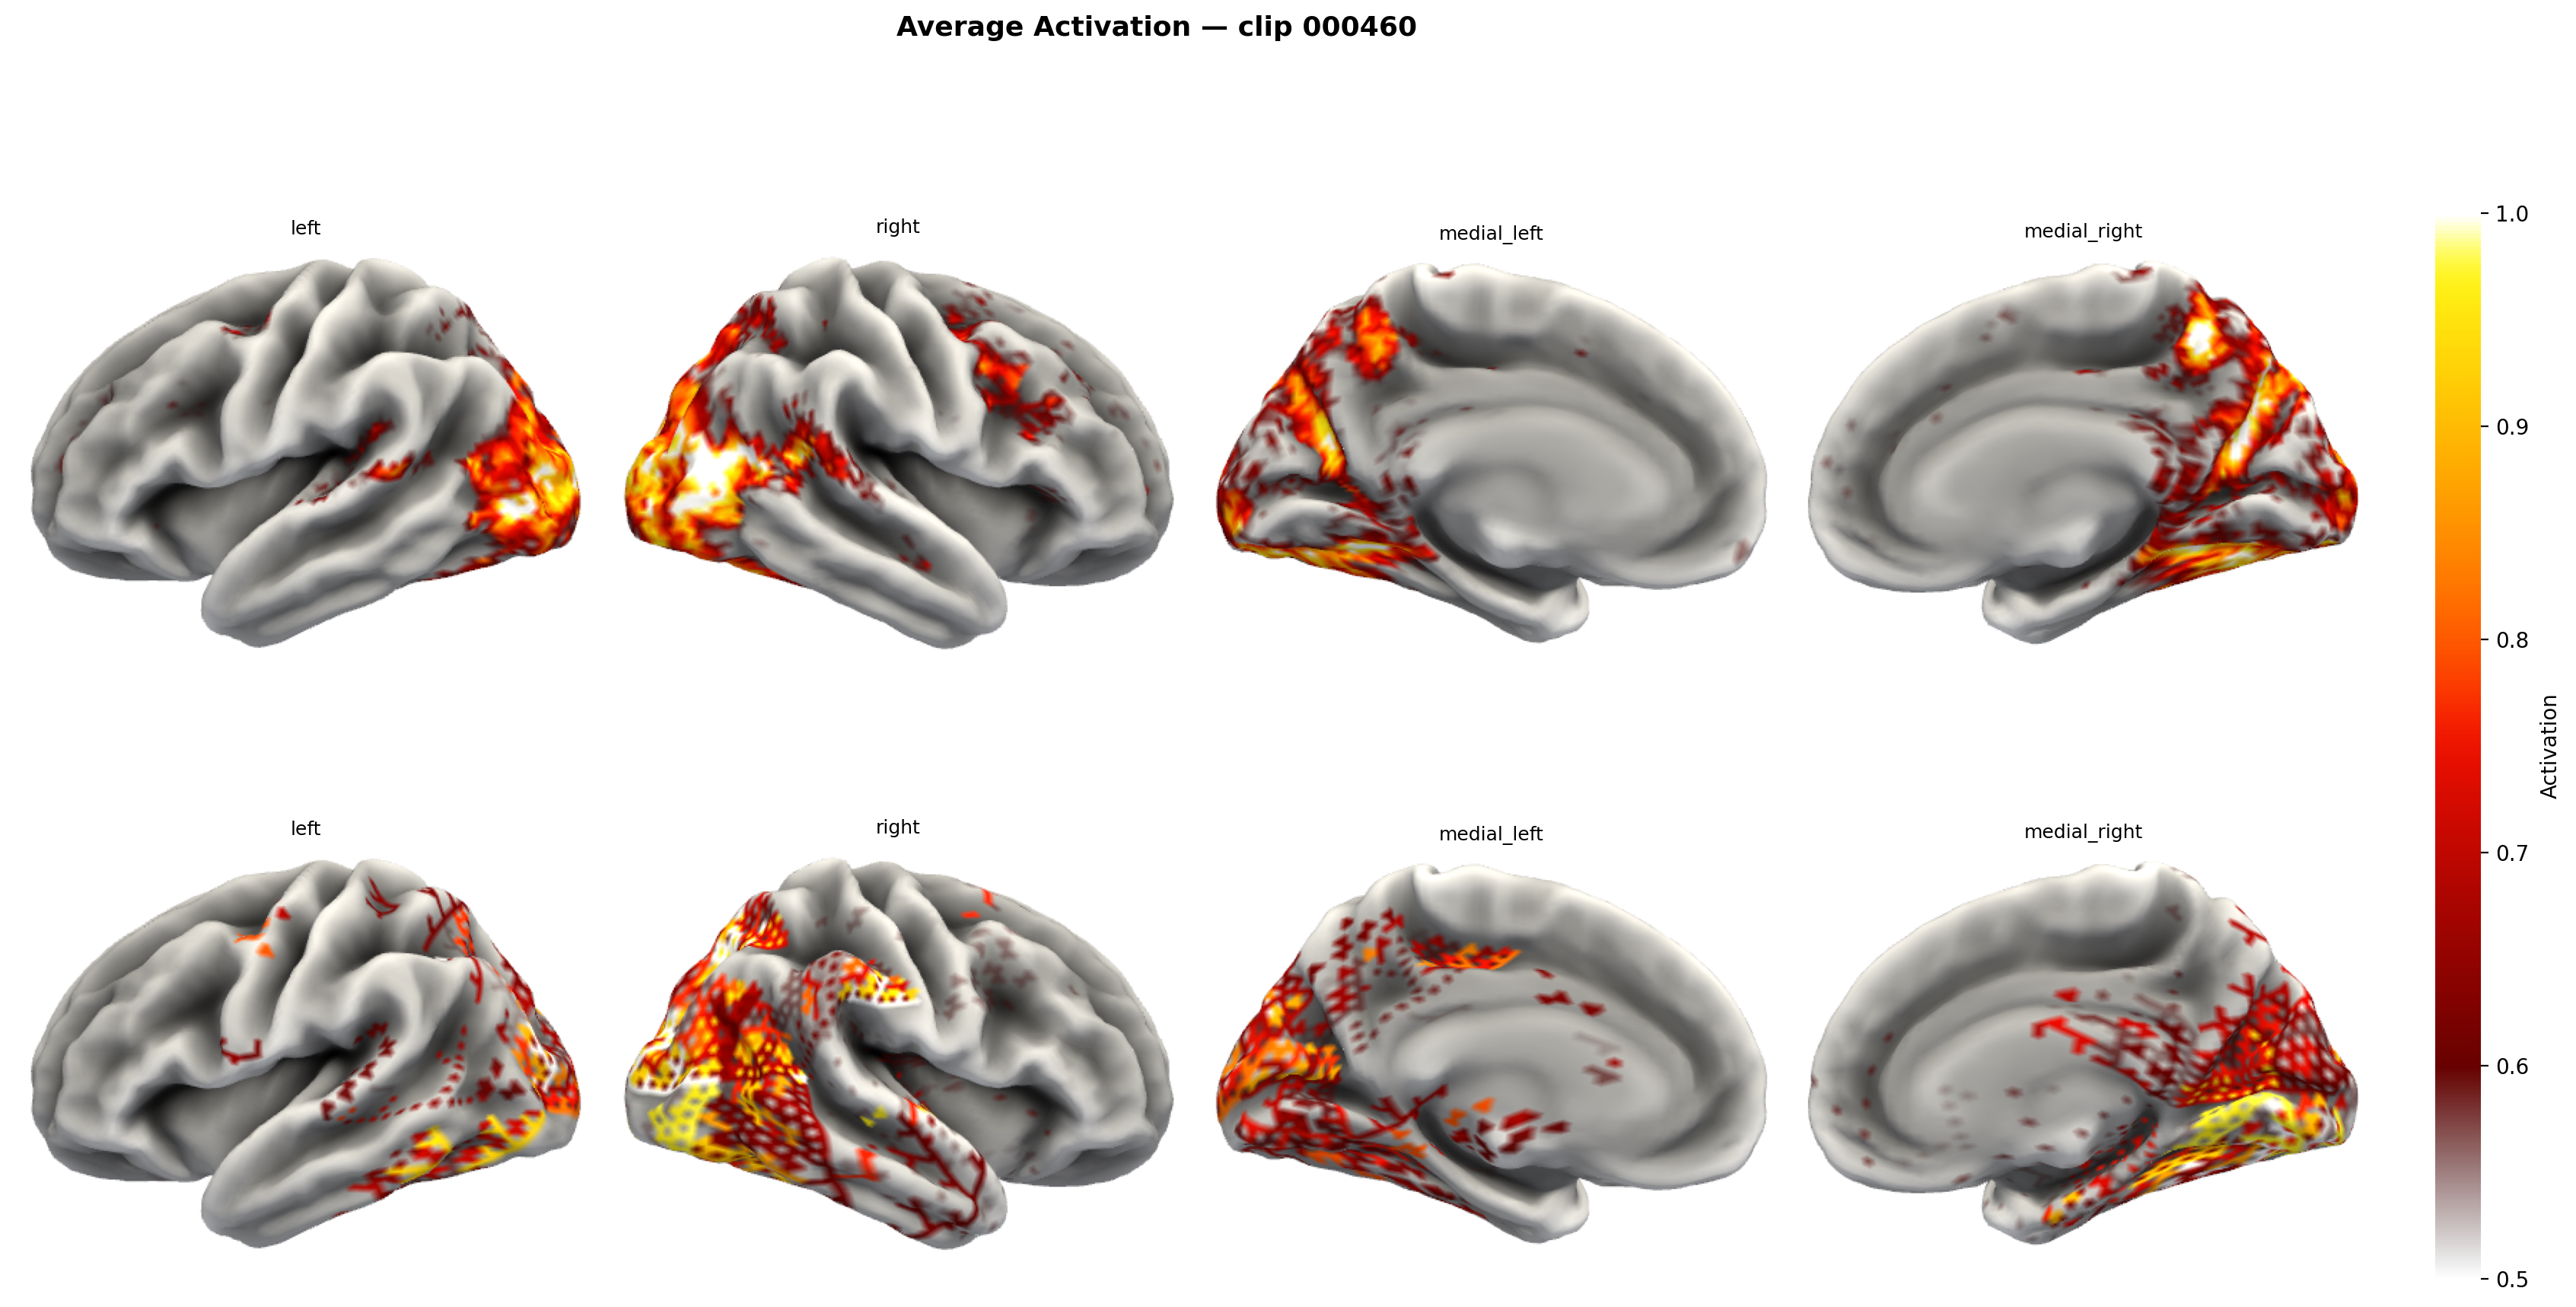
\includegraphics[width=\textwidth]{plots/brain_viz_000460_activation_map.png}
\caption{Клип 000460}
\end{subfigure}
\caption{Дополнительные предсказанные карты кортикальной
активности (\texttt{plots/brain\_viz\_*\_activation\_map.png}).}
\label{fig:moreclips}
\end{figure}

\section{Реестр пробелов данных}
\label{app:gaps}

\begin{table}[H]
\centering
\caption{Данные, отсутствующие в проекте и необходимые для
полной публикации.}
\label{tab:gaps}
\small
\begin{tabular}{p{0.62\textwidth}p{0.3\textwidth}}
\toprule
Пробел & Где закрыть \\
\midrule
Поэпохальный лог обучения (рис.~\ref{fig:training} схематичен) &
TensorBoard \texttt{tb\_logs} \\
Абляции компонентов (HRF, MoE, гейтинг, FiLM); sparse-варианты &
\texttt{v3\_benchmark\_sparse.py} \\
Тесты значимости: нулевое распределение, FDR, шумовой потолок &
протокол~\cite{Huth2016} \\
Результаты Phase~1 (претрейнинг) и Phase~3 (реальный фМРТ) &
\texttt{v3\_pipeline.py} \\
Точное fsaverage5 $\rightarrow$ Schaefer-400 соответствие (.annot) &
\texttt{parcellate()} \\
Демография субъектов 200-клипового корпуса; подтверждение TR &
документация CINE Brain \\
\bottomrule
\end{tabular}
\end{table}

\section{Программный код и воспроизводимость}
\label{app:repo}

Полный исходный код модели, обучения и инференса открыт и доступен:
\begin{center}
\url{https://github.com/qaddasd/Flora}
\end{center}

Структура:
\begin{itemize}[leftmargin=*]
    \item \texttt{flora/v3\_model.py}~--- модель FloraV3 (проекторы,
          MoE-трансформер, HRF, FiLM);
    \item \texttt{flora/v3\_train.py}, \texttt{train\_lightning.py}~---
          процедуры обучения (PyTorch Lightning);
    \item \texttt{flora/v3\_pretrain.py}~--- самообучаемый
          претрейнинг;
    \item \texttt{flora/extract\_features\_v3.py}~--- извлечение
          мультимодальных признаков;
    \item \texttt{flora/backbones.py}~--- обёртки замороженных
          энкодеров (MiniLM, Whisper-Tiny, MobileViT-S);
    \item \texttt{flora/config.py}~--- конфигурация;
    \item \texttt{run\_flora.py}~--- CLI инференса на видеофайле;
    \item \texttt{scripts/benchmark\_flora.py}~--- бенчмарк
          (\cref{sec:benchmarks}).
\end{itemize}

\section{Этические замечания}
\label{app:ethics}

Все эксперименты в настоящей работе выполнены на открытом
нейровизуализационном корпусе CINE Brain~\cite{Gao2025cinebrain},
полученном с информированным согласием участников и одобренным
соответствующим этическим комитетом. Авторы настоящей работы не
собирали первичных данных о здоровье; модель обучена только на
публично доступных измерениях.

Любое практическое применение компактных моделей мозга для
клинических или коммерческих целей должно сопровождаться
этической экспертизой и соблюдением местного законодательства о
защите персональных данных и биомедицинских исследованиях.

\end{document}
